\chapter{Ordered abstract machines}
\label{chapter-absmachine}

This chapter centers around two transformations on logical
specifications.  Taken together, the operationalization transformation
(Section~\ref{sec:operationalization}) and the defunctionalization
transformation (Section~\ref{sec:defunctionalization}) allow us to
establish the logical correspondence between the deductive SLS
specification of a natural semantics and the concurrent SLS
specification of an abstract machine.

Natural semantics specifications are common in the literature,
and are also easy to encode in either the deductive fragment of
\sls~or in a purely deductive logical framework like LF.  We will
continue to use the natural semantics specification of call-by-value
evaluation for the lambda calculus as a running example:
\[
\infer[{\sf ev/lam}]
{\obj{\lambda x. e \Downarrow \lambda x. e} \mathstrut}
{}
\quad
\infer[{\sf ev/app}]
{\obj{e_1\,e_2 \Downarrow v} \mathstrut}
{\obj{e_1 \Downarrow \lambda x.e}
 &
 \obj{e_2 \Downarrow v_2}
 &
 \obj{[v_2/x]e \Downarrow v} \mathstrut}
\]
Natural semantics are a {\it big-step} semantics: the judgment
$\obj{e \Downarrow v}$ describes the relationship between an 
initial expression
$\obj{e}$ and the value $\obj{v}$ to which it will eventually evaluate.

The alternative to a big-step semantics is a {\it small-step}
semantics, which describes the relationship between one intermediate
state of a computation and another intermediate state after a
single transition. One form of small-step semantics is a structural
operational semantics (SOS) specification
\cite{plotkin04structural}. The SOS specification of call-by-value
evaluation for the lambda calculus is specified in terms of two
judgments: $\obj{v\,{\sf value}}$, which expresses that $\obj{v}$ is a
value that is not expected to make any more transitions, and $\obj{e_1
  \mapsto e_2}$, which expresses that $\obj{e_1}$ transitions to 
$\obj{e_2}$ by reducing a $\beta$-redex. 
\[
\infer
{\obj{\lambda x.e\,{\sf value}} \mathstrut}
{}
\quad
\infer
{\obj{e_1\,e_2 \mapsto e_1'\,e_2} \mathstrut}
{\obj{e_1 \mapsto e_1'} \mathstrut}
\quad
\infer
{\obj{e_1\,e_2 \mapsto e_1\,e_2'} \mathstrut}
{\obj{e_1\,{\sf value}}
 &
 \obj{e_2 \mapsto e_2'} \mathstrut}
\quad
\infer
{\obj{(\lambda x. e)v \mapsto [v/x]e} \mathstrut}
{\obj{v\,{\sf value}} \mathstrut}
\]

Abstract machine semantics are another important small-step semantics
style. The most well-known abstract semantics is almost certainly
Landin's SECD machine \cite{landin64mechanical}, though our abstract
machine presentation below is much closer to Danvy's SC machine from
\cite{danvy03rational} and Harper's $\mathcal K\{{\sf
  nat}{\rightharpoonup}\}$ system from \cite[Chapter
27]{harper12practical}.  This abstract machine semantics is defined in
terms of states $\obj{s}$. The state $\obj{s} = \obj{k \rhd e}$
represents the expression $\obj{e}$ being evaluated on top of the
stack $\obj{k}$, and the state $\obj{s} = \obj{k \lhd v}$ represents
the value $\obj{v}$ being returned to the stack $\obj{k}$. Stacks
$\obj{k}$ are have the form $\obj{((\ldots({\sf halt}; f_1); \ldots);
  f_n)}$ -- they are left-associative sequences of frames $\obj{f}$
terminated by $\obj{\sf halt}$, where $\obj{{\sf halt} \rhd e}$ is the
initial state in the evaluation of $\obj{e}$ and 
$\obj{{\sf halt} \lhd v}$ is a final
state that has completed evaluating to a value 
$\obj{v}$.  Each frame $\obj{f}$ either has the form $\obj{\Box\,e_2}$
(an application frame waiting for an evaluated function to be returned
to it) or the form $\obj{(\lambda x.e)\,\Box}$ (an application frame
with an evaluated function waiting for an evaluated value to be
returned to it). Given states, stacks, and frames, we can define a
``classical'' abstract machine for call-by-value evaluation of the
lambda calculus as a transition system with four transition rules:
\begin{align*}
{\sf absmachine/lam}{:} & ~~ 
 \obj{k \rhd \lambda x.e ~ \mapsto ~ k \lhd \lambda x.e}
\\
{\sf absmachine/app}{:} & ~~ 
 \obj{k \rhd e_1\,e_2 ~ \mapsto ~ (k; \Box\,e_2) \rhd e_1}
\\
{\sf absmachine/app1}{:} & ~~ 
 \obj{(k; \Box\,e_2) \lhd \lambda x.e ~ 
   \mapsto ~ (k; (\lambda x.e)\,\Box) \rhd e_2}
\\
{\sf absmachine/app2}{:} & ~~
 \obj{(k; (\lambda x.e)\,\Box) \lhd v_2 ~ \mapsto ~ k \rhd [v_2/x]e}
\end{align*}

The operational intuition for these rules is precisely the same as the
operational intuition for the rewriting rules given in
Section~\ref{sec:intro-ssos}. This is not coincidental: the
\sls~specification from the introduction adequately encodes the
transition system $\obj{s \mapsto s'}$ defined above, a point that we will
make precise in Section~\ref{sec:nat-ssos-adequacy}. The
\sls~specification from the introduction is {\it also} the result of
applying the operationalization and defunctionalization
transformations to the \sls~encoding of the natural semantics given
above. Therefore, these two transformations combined with the adequacy
arguments at either end constitute a logical correspondence between
natural semantics and abstract machines. 

As discussed in Section~\ref{sec:the-point-is-modular-extension}, it
is interesting to put existing specification styles into logical
correspondence, but that is not our main reason for investigating
logical correspondence in the context of this thesis. Rather, we are
primarily interested in exploring the set of programming language
features that can be modularly integrated into a transformed
\sls~specification and that could {\it not} be integrated into a natural
semantics specification in a modular fashion.  
In Section~\ref{sec:richer-ordered-abstract}
we explore a selection of these features, including mutable storage,
call-by-need evaluation, and recoverable failure.

\section{Logical transformation: operationalization}
\label{sec:operationalization}

The intuition behind operationalization is rather simple: we examine
the structure of backward chaining and then specify that
computational process as an \sls~specification.  Before presenting
the general transformation, we will motivate this transformation using
our natural semantics specification of call-by-value evaluation. 

The definition of $\obj{e \Downarrow v}$ is moded with $\obj{e}$ as an
input and $\obj{v}$ as an output, so it is meaningful to talk about
being given $\obj{e}$ and using deductive computation to search for a
$\obj{v}$ such that $\obj{e \Downarrow v}$ is derivable.  Consider a
recursive search procedure implementing this particular deductive
computation: 
\smallskip
\begin{itemize}
\item
      If $\obj{e} = \obj{\lambda x. e'}$, 
      it is possible to derive 
      $\obj{\lambda x. e' \Downarrow \lambda x. e'}$
      with the rule ${\sf ev/lam}$.
\item
       If $\obj{e} = \obj{e_1\,e_2}$,
       attempt to derive 
       $\obj{e_1\,e_2 \Downarrow v}$
       using the rule ${\sf ev/app}$ by doing the following:
    \begin{enumerate}
    \item Search for a $\obj{v_1}$ such that 
          $\obj{e_1 \Downarrow v_1}$ is derivable.
    \item Assess whether $\obj{v_1} = \obj{\lambda x.e'}$ for some
          $\obj{e'}$; fail if it is not.
    \item Search for a $\obj{v_2}$ such that 
          $\obj{e_2 \Downarrow v_2}$ is derivable.
    \item Compute $\obj{e'} = \obj{[v_2/x]e}$
    \item Search for a $\obj{v}$ such that 
          $\obj{e' \Downarrow v}$ is derivable.
    \end{enumerate}
% \item
%       If $e = e_1 \arb e_2$,
%       attempt to derive $e_1 \arb e_2 \Downarrow v$ using
%       the rule ${\sf ev/choose1}$ by searching for a 
%       $v$ such that $e_1 \Downarrow v$ is derivable.
% \item
%       If $e = e_1 \arb e_2$,
%       attempt to derive $e_1 \arb e_2 \Downarrow v$ using 
%       the rule ${\sf ev/choose2}$ by searching for a 
%       $v$ such that $e_2 \Downarrow v$ is derivable.  
\end{itemize}
\smallskip
%
The goal of the operationalization transformation is to represent this
deductive computation as a specification in the concurrent fragment of
\sls. (To be sure, ``concurrent'' will seem 
like a strange word to use at first, as
the specifications we write in the concurrent fragment of \sls~will 
be completely sequential until Section~\ref{sec:trans-par}.)
The first step in this process, representing the syntax
of expressions as LF terms of type ${\sf exp}$, was discussed
in Section~\ref{sec:lf-adequacy}. The second step is to
introduce two new ordered atomic propositions.  The proposition ${\sf
  eval}\,\interp{e}$ is the starting point, indicating that we want to
search for a $\obj{v}$ such that $\obj{e \Downarrow v}$,
 and the proposition ${\sf
  retn}\,\interp{v}$ indicates the successful completion of this
procedure. Therefore, searching for a $\obj{v}$ such that 
$\obj{e \Downarrow v}$
is derivable will be analogous to building a trace $T ::
x_e{:}\susp{{\sf eval}\,\interp{e}} \leadsto^* x_v{:}\susp{{\sf
    retn}\,\interp{v}}$.

Representing the first case is straightforward: if we are evaluating
$\obj{\lambda x.e}$, then we have succeeded and can return
$\obj{\lambda x.e}$.  This is encoded as the following proposition:
\[
\forall \lf{E}.\,
{\sf eval}\,\lf{({\sf lam}\,\lambda x.\,E\,x)}
   \lefti \{ {\sf retn}\,\lf{({\sf lam}\,\lambda x.\,E\,x)} \}
\]
The natural deduction rule ${\sf ev/app}$ involves both recursion and
multiple subgoals. The five steps in our informal search procedure are
turned into three phases in \sls, corresponding to the three recursive
calls to the search procedure -- steps 1 and 2 are combined, as are
steps 4 and 5. Whenever we make a recursive call to the search
procedure, we leave a negative ordered proposition $\istrue{A^-}$ in
the context that awaits the return of a proposition ${\sf
  retn}\,\interp{v'}$ to its left and then continues with the search
procedure. Thus, each of the recursive calls to the search procedure
will involve a sub-trace of the form
%
\[x_e{:}\susp{{\sf eval}\,\interp{e'}}, y{:}\istrue{A^-}, \Delta
  \leadsto^*
  x_v{:}\susp{{\sf retn}\,\interp{v'}}, y{:}\istrue{A^-}, \Delta
\]
%
where $A^-$ is a negative proposition that is prepared to interact
with the subgoal's final ${\sf retn}\,\interp{v'}$ proposition to
kickstart the rest of the computation.  This negative proposition is,
in effect, the calling procedure's continuation.

The nested rule for evaluating $\obj{e_1\,e_2}$ to a value is the
following proposition,
where the three phases are indicated with dashed boxes:

\begin{center}
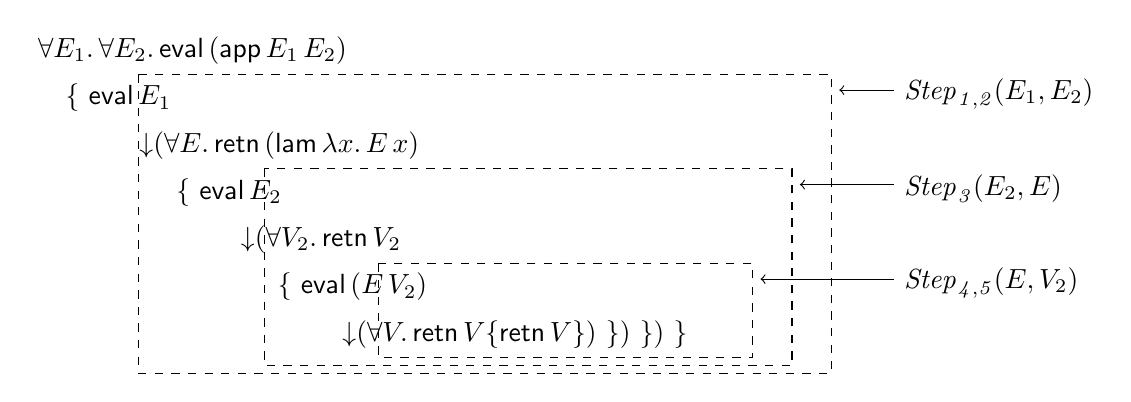
\begin{tikzpicture}
\draw (5,0) node[right]{$\forall \lf{E_1}.\,\forall \lf{E_2}.\,
         {\sf eval}\,\lf{({\sf app}\,E_1\,E_2)}$};
\draw (5,-.6) node[right]{\quad 
   $\lefti \{ ~ {\sf eval}\,\lf{E_1} \fuse ~$};
\draw (5,-1.2) node[right]{\quad\qquad ~
   $ {\downarrow}
     (\forall \lf{E}.\, {\sf retn}\,\lf{({\sf lam}\,\lambda x.\,E\,x)}$};
\draw (5,-1.8) node[right]{\qquad\qquad ~~
   $\lefti \{ ~ {\sf eval}\,\lf{E_2} \fuse ~$};
\draw (5,-2.4) node[right]{\qquad\qquad\qquad ~~~
   $ {\downarrow}
     (\forall \lf{V_2}.\, {\sf retn}\,\lf{V_2}$};
\draw (5,-3) node[right]{\qquad\qquad\qquad\quad ~~~~
   $\lefti \{ ~ {\sf eval}\,\lf{(E\,V_2)} \fuse ~$};
\draw (5,-3.6) node[right]{\qquad\qquad\qquad\qquad\quad ~~~~~
   $ {\downarrow}(\forall \lf{V}.\, {\sf retn}\,\lf{V}
      \lefti \{ {\sf retn}\,{\lf V}\})~\})~\})~\}$};

\draw[dashed] (9.45, -2.7) -- (9.45,-3.9) -- (14.2,-3.9) -- (14.2,-2.7)
           -- (9.45, -2.7);
\draw[dashed] (8, -1.5) -- (8, -4) -- (14.7,-4) -- (14.7,-1.5)
           -- (8, -1.5);
\draw[dashed] (6.4, -.3) -- (6.4, -4.1) -- (15.2, -4.1) -- (15.2, -.3)
           -- (6.4, -.3); 

\draw[<-] (15.3, -.5) -- (16, -.5); 
\draw (16, -.55) node[right]{${\it Step}_{\it 1,2}(\lf{E_1},\lf{E_2})$};
\draw[<-] (14.8, -1.7) -- (16, -1.7);
\draw (16, -1.75) node[right]{${\it Step}_{\it 3}(\lf{E_2},\lf{E})$};
\draw[<-] (14.3, -2.9) -- (16, -2.9);
\draw (16, -2.95) node[right]{${\it Step}_{\it 4,5}(\lf{E},\lf{V_2})$};
%   \lefti \{ {\sf retn}\,\lf{({\sf lam}\,\lambda x.\,E\,x)} \}
\end{tikzpicture}
\end{center}

% We will establish a calling convention for recursive calls to the
% search procedure. Whenever, in the course of constructing
% $x_e{:}\susp{{\sf eval}\,\interp{e_1\,e_2}}, \Delta \leadsto^*
% x_v{:}\susp{{\sf retn}\,\interp{v}}, \Delta$, we need to recursively
% call the search procedure on some other expression $\interp{e'}$, we
% will leave a negative ordered proposition $\istrue{A^-}$ in the
% context that awaits the return of a proposition ${\sf
%   retn}\,\interp{v'}$ to its left and then continues with the search
% procedure. Thus, each of the recursive calls to the search procedure
% will involve a sub-trace of the form
% %
% \[x_e{:}\susp{{\sf eval}\,\interp{e'}}, y{:}\istrue{A^-}, \Delta
%   \leadsto^*
%   x_v{:}\susp{{\sf retn}\,\interp{v'}}, y{:}\istrue{A^-}, \Delta\]
% %
%   where $A^-$ is a negative proposition that is prepared to interact
%   with the subgoal's final ${\sf retn}\,\interp{v'}$ proposition to
%   kickstart the rest of the computation.  This negative proposition
%   is, in effect, the calling procedure's continuation.

\noindent
Let's work backwards through this three-phase protocol.  In the third
phase, which corresponds to the fourth and fifth steps of our informal
search procedure, we have found $\lf{\lambda x.\,E\,x} = \lf{\lambda
  x.\interp{e}}$ (where $\obj{e}$ potentially has $\obj{x}$ free) and
$\lf{V_2} = \interp{v_2}$. The recursive call is to ${\sf
  eval}\,\interp{[v_2/x]e}$, which is the same thing as ${\sf
  eval}\,\lf{(E\,V_2)}$. If the recursive call successfully returns,
the context will contain a suspended atomic proposition of the form
${\sf retn}\,\lf{V}$ where $\lf{V} = \interp{v}$, and the search
procedure as a whole has been completed: the answer is $\obj{v}$.
Thus, the negative proposition that implements the continuation can be
written as $(\forall \lf{V}.\,{\sf retn}\,\lf{V} \lefti \{ {\sf
  retn}\,\lf{V} \})$. (This continuation is the identity; we
will show how to omit it when we discuss tail-recursion elimination in
Section~\ref{sec:trans-tail}.)  The positive proposition that will
create this sub-computation can be written as follows:
\begin{align*}
{\it Step_{4,5}}(\lf{E},\lf{V_2}) & \equiv {\sf eval}\,\lf{(E\,V_2)} 
\fuse {\downarrow}(\forall \lf{V}.\, {\sf retn}\,\lf{V} \lefti \{ {\sf retn}\,\lf{V} \})
%
\intertext{Moving backwards, in the second phase (step 3 of the 5-step
procedure)
we have an expression $\lf{E_2} =
  \interp{e_2}$ that we were given and $\lf{\lambda x.\,E\,x} = \lf{\lambda x.\interp{e}}$ that we
  have computed. The recursive call is to ${\sf
    eval}\,\interp{e_2}$, and assuming that it completes, we need
  to begin the fourth step. The positive proposition that will 
  create this sub-computation can be written as follows:}
%
{\it Step_3}(\lf{E_2},\lf{E}) & \equiv {\sf eval}\,\lf{E_2} 
\fuse {\downarrow}(\forall \lf{V_2}.\,
  {\sf retn}\,\lf{V_2} \lefti \{ {\it Step_{4,5}}(\lf{E},\lf{V_2}) \})
%
\intertext{Finally, the first two steps, like the fourth and fifth steps,
are handled together. We have
$\lf{E_1} = \interp{e_1}$ and $\lf{E_2} = \interp{e_2}$; the recursive
call is to ${\sf eval}\,\interp{e_1}$. Once the
recursive call completes, we enforce that the returned value has
the form $\interp{\lambda x.e}$ before proceeding
to the continuation.}
{\it Step_{1,2}}(\lf{E_1}, \lf{E_2}) & \equiv {\sf eval}\,\lf{E_1}
\fuse {\downarrow}(\forall \lf{E}.\, {\sf retn}\,\lf{({\sf lam}\,\lambda x.\,E\,x)}
\lefti \{ {\it Step_3}(\lf{E_2}, \lf{E})\})
\end{align*}
Thus, the rule implementing this entire portion of the search
procedure is 
\[
\forall \lf{E_1}.\,\forall \lf{E_2}.\,
{\sf eval}\,\lf{({\sf app}\,E_1\,E_2)} \lefti \{ {\it
  Step_{1,2}}(\lf{E_1}, \lf{E_2}) \}
\]

The \sls~encoding of our example natural semantics is shown in
Figure~\ref{fig:example-transform-cbv} alongside the transformed
specification, which has the form of an ordered abstract machine
semantics, though it is different than the ordered abstract machine
semantics presented in the introduction. The specification in 
Figure~\ref{fig:example-transform-cbv} is 
{\it nested}, as ${\sf ev/app}$ is a rule that, when it
participates in a transition, produces a new rule $(\forall
\lf{E}.\,{\sf retn}\,\lf{({\sf lam}\,\lambda x.\,E\,x)} \lefti \{
\ldots \})$ that lives in the context. (In contrast, the ordered
abstract machine semantics from the introduction was {\it flat}.)  We
discuss the defunctionalization transformation, which allows us to
derive flat specifications from nested specifications, in
Section~\ref{sec:defunctionalization} below.

\begin{figure}
\begin{minipage}[b]{0.36\linewidth}
\fvset{fontsize=\small,boxwidth=auto}
\VerbatimInput{sls/cbv-ev.sls}
\end{minipage}
\hspace{0.5cm}
\begin{minipage}[b]{0.64\linewidth}
\fvset{fontsize=\small,boxwidth=auto}
\VerbatimInput{sls/cbv-ev-ssos.sls}
\end{minipage}
\caption{Natural semantics (left) and ordered abstract machine (right) for 
CBV evaluation}
\label{fig:example-transform-cbv}
\end{figure}

The intuitive connection between natural semantics specifications and
concurrent specifications has been explored previously and
independently in the context of CLF by Schack-Nielsen
\cite{schacknielsen07induction} and by Cruz and Hou
\cite{cruz12parallel}; Schack-Nielsen proves the equivalence of the
two specifications, whereas Cruz and Hou used the connection
informally. The contribution of this section is to describe a general
transformation (of which Figure~\ref{fig:example-transform-cbv} is one
instance) and to prove the transformation correct in general. We have
implemented the operationalization
and defunctionalization transformations within the prototype
implementation of \sls.

In Section~\ref{sec:trans-subset} we will present the subset of
specifications that our operationalization transformation handles, and
in Section~\ref{sec:trans-basic} we present the most basic form of the
transformation.  In
Sections~\ref{sec:trans-tail}~and~\ref{sec:trans-par} we extend the
basic transformation to be both tail-recursion optimizing and
parallelism-enabling. Finally, in
Section~\ref{sec:operationalization-correct}, we establish the
correctness of the overall transformation.

\subsection{Transformable signatures}
\label{sec:trans-subset}

The starting point for the operationalization transformation is a
deductive signature that is well-moded in the sense described in
Section~\ref{sec:framework-modes}. Every declared negative predicate
will either remain defined by deductive proofs (we write the atomic
propositions built with these predicates as $p_d^-$, $d$ for
deductive) or will be transformed into the concurrent fragment of
\sls~(we write these predicates as ${\sf a_c}$, ${\sf b_c}$ etc.~and
write the atomic propositions built with these predicates as $p_c^-$,
$c$ for concurrent).

For the purposes of describing and proving the correctness of the
operationalization transformation, we will assume that all transformed
atomic propositions $p_c^-$ have two arguments where the first
argument is moded as an input and the second is an output. That is,
they are declared as follows:
\begin{align*}
& {\sf \#mode~a_c~{+}~{-}}.\\
& {\sf a_c} : \tau_1 \rightarrow \tau_2 \rightarrow {\sf prop}.
\end{align*}
Without dependency, two-place relations are sufficient for describing
$n$-place relations.\footnote{As an example, consider addition
   defined as a three-place relation ${\sf
    add}\,\lf{M}\,\lf{N}\,\lf{P}$ (where ${\sf add}$ has kind ${\sf
    nat} \rightarrow {\sf nat} \rightarrow {\sf nat} \rightarrow {\sf
    prop}$) with the usual mode (${\sf add}~{+}~{+}~{-}$). We can
  instead use a two-place relation ${\sf add'}\,\lf{({\sf
      add\_inputs}\,M\,N)}\,\lf{P}$ with mode (${\sf add'}~{+}~{-}$). The
  kind of ${\sf add'}$ is ${\sf add\_in} \rightarrow {\sf nat}
  \rightarrow {\sf type}$, where ${\sf add\_in}$ is a new type with
  only one constructor ${\sf add\_inputs} : {\sf nat} \rightarrow {\sf nat}
  \rightarrow {\sf add\_in}$ that effectively pairs together the two natural
  numbers that are inputs.}  It should be possible to handle dependent predicates
(that is, those with declarations of the form ${\sf a_c} : \Pi
\lf{x}{:}\tau_1.\,\tau_2(\lf{x}) \rightarrow {\sf type}$), but we will not do so
here.

The restriction on signatures furthermore enforces that all rules must
be of the form ${\sf r} : C$ or ${\sf r} : D$, where $C$ and $D$ are
refinements of the negative propositions of \sls~that are defined as
follows:
\begin{align*}
C & ::= p^-_{c} 
    \mid \forall \lf x{:}\tau.\, C
    \mid p^+_\mpers \lefti C
    \mid {!}p^-_c \lefti C
    \mid {!}G \lefti C \\
D & ::= p^-_{d}
    \mid \forall \lf x{:}\tau.\, D
    \mid p^+_\mpers \lefti D
    \mid {!}p^-_c \lefti D
    \mid {!}G \lefti C \\
G & ::= p^-_d 
    \mid \forall \lf x{:}\tau.\, G
    \mid p^+_\mpers \lefti G
    \mid {!}D \lefti G
\end{align*}
For most of this chapter, we will 
restrict our attention to signatures where all atomic
propositions have the form $p^-_c$ and where all rules have the form
$C$. This makes the classes $p^-_d$, $D$, and $G$ irrelevant and
effectively restricts rules to the Horn fragment.  Propositions
$p^-_d$ that remain deductively defined by rules $D$ will only be
considered towards the end of this chapter in
Section~\ref{sec:evaluationcontexts} when we consider various
transformations on SOS specifications and in
Section~\ref{sec:lambdacircle} when we consider transforming the
natural semantics for Davies' \rowan.

Note, however, that if a signature is well-formed given that a certain
atomic proposition is assigned to the class $p^-_c$ of transformed
atomic propositions, the signature will {\it remain} well-formed if we
instead assign that proposition to the class $p^-_d$ of atomic
propositions that get left in the deductive fragment. The only effect
is that some rules that were previously of the form ${\sf r} : C$ will
become rules of the form ${\sf r} : D$.\footnote{The reverse does not
  hold: the proposition ${!}(\forall\lf{x}{:}\tau.\,p^+_\mpers \lefti
  p^-_d) \lefti p^-_d$ has the form $D$, but the proposition
  ${!}(\forall\lf{x}{:}\tau.\,p^+_\mpers \lefti p^-_c) \lefti p^-_c$
  does {\it not} have the form $C$.} If we turn this dial all the way,
we won't operationalize anything! If {\it all} atomic propositions are
of the form $p^-_d$ so that they remain deductive, then the
propositions $p^-_c$ and $C$ are irrelevant, and the restriction above
describes all persistent, deductive specifications -- essentially, any
signature that could be executed by the standard logic programming
interpretation of LF \cite{pfenning89elf}. The operationalization
transformation will be the identity on such a specification.

All propositions $C$ are furthermore equivalent (at the
level of synthetic inference rules) to propositions of the form
$\forall \lf{\overline{x_0}}\ldots \forall \lf{\overline{x_n}}.\,A^+_n
\lefti \ldots \lefti A^+_1 \lefti {\sf
  a_c}\,\lf{t_{0}}\,\lf{t_{n+1}}$, where the $\forall
\lf{\overline{x_i}}$ are shorthand for a series of universal
quantifiers $\forall \lf{x_{i1}}{:}{\tau_{i1}} \ldots \forall
\lf{x_{\it ik}}{:}{\tau_{\it ik}}$, and where each variable in
$\lf{\overline{x_i}}$ does not appear in $\lf{t_0}$ (unless $i = 0$)
nor in any $A^+_j$ with $j < i$ but does appear in $A^+_i$ (or
$\lf{t_0}$ if $i = 0$). Therefore, when we consider moded proof
search, the variables bound in $\lf{\overline{x_0}}$ are all fixed by
the query and those bound in the other $\lf{\overline{x_i}}$ are all
fixed by the output position of the $i^{\rm th}$ subgoal.

Each premise $A^+_i$ either has the form
$p^+_\mpers$, ${!}p^-_c$, or ${!}G$. The natural deduction rule ${\sf ev/app}$,
which has three premises,
can be represented in this standard form as follows: 
\vspace{-10pt}
\begin{center}
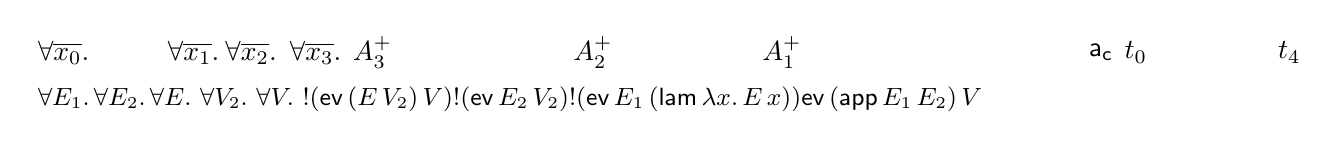
\begin{tikzpicture}
\draw (0,1.6) node[right]{$\forall \lf{\overline{x_0}}.$};
\draw (1.65,1.6) node[right]{$\forall \lf{\overline{x_1}}.$};
\draw (2.38,1.6) node[right]{$\forall \lf{\overline{x_2}}.$};
\draw (3.2,1.6) node[right]{$\forall \lf{\overline{x_3}}.$};
\draw (4,1.6) node[right]{$A^+_3 \lefti $};
\draw (6.8,1.6) node[right]{$A^+_2 \lefti $};
\draw (9.2,1.6) node[right]{$A^+_1 \lefti $};
\draw (13.35,1.6) node[right]{$\sf a_c$};
\draw (13.8,1.6) node[right]{$\lf{t_0}$};
\draw (15.75,1.6) node[right]{$\lf{t_{4}}$};
\draw (0,1) 
 node[right]{\small 
           $\forall \lf{E_1}.\, 
            \forall \lf{E_2}.\,
            \forall \lf{E}.~
            \forall \lf{V_2}.~
            \forall \lf{V}.~
            {!}({\sf ev}\,\lf{(E\,V_2)}\,\lf{V}) \lefti
            {!}({\sf ev}\,\lf{E_2}\,\lf{V_2}) \lefti
            {!}({\sf ev}\,\lf{E_1}\,\lf{({\sf lam}\,\lambda x.\,E\,x)}) \lefti
            {\sf ev}\,\lf{({\sf app}\,E_1\,E_2)}\,\lf{V}$};
\end{tikzpicture}
\end{center}
From here on out we will assume without loss of generality that any
proposition $C$ actually has this very specific form.


\subsection{Basic transformation}
\label{sec:trans-basic}

The operationalization transformation $\transop{\Sigma}$
operates on SLS signatures $\Sigma$ that have the form described in the
previous section. We
will first give the transformation on signatures; the transformation
of rule declarations ${\sf r} : C$ is the key case.

Each two-place predicate ${\sf a_c}$ gets associated with two
one-place
predicates ${\sf eval\_a}$ and ${\sf retn\_a}$: both ${\sf
  eval\_a}\,t$ and ${\sf retn\_a}\,t$ are positive ordered atomic
propositions. 
We will write $\opsubst{X}$ for the operation of
substituting all occurrences of $p^-_c = {\sf a_c}\,t_1\,t_2$ with
$({\sf eval\_a}\,t_1 \lefti \{ {\sf retn\_a}\,t_2 \})$ in $X$. This
substitution operation is used on propositions and contexts;
it appears in the transformation of rules ${\sf r} : D$ below.

\smallskip
\begin{itemize}
\item $\transop{\cdot} = \cdot$
\item $\transop{\Sigma, {\sf a_c} : \tau_1 \rightarrow \tau_2
    \rightarrow {\sf prop}} = \transop{\Sigma}, ~ {\sf eval\_a} :
  \tau_1 \rightarrow {\sf prop\,ord}, ~ {\sf retn\_a} : \tau_2
  \rightarrow {\sf prop\,ord}$ 
\item $\transop{\Sigma, {\sf a_c} : \tau_1 \rightarrow \tau_2
    \rightarrow {\sf prop}} = \transop{\Sigma}, ~ {\sf eval\_a} :
  \tau_1 \rightarrow {\sf prop\,ord}$ \\
{\it (if ${\sf retn\_a}$ is already defined)}
\item $\transop{\Sigma, {\sf b} : \kappa} = \transop{\Sigma}, ~ {\sf b}
  : \kappa$ {\it (if ${\sf b} \neq {\sf a_c}$)}
\item $\transop{\Sigma, \lf{\sf c} : \tau} = \transop{\Sigma}, ~ \lf{\sf
    c} : \tau$ 
\item $\transop{\Sigma, {\sf r} : C} = \transop{\Sigma}, ~ {\sf r}
  : \forall \lf{\overline{x_0}}.\, {\sf eval\_a}\,\lf{t_0} \lefti 
      \opbasic{A^+_1, \ldots, A^+_n}{\lf{t_{n+1}}}{\lf{\sf id}}$ \\ 
    {\it (where $C = \forall \lf{\overline{x_0}}\ldots \forall
    \lf{\overline{x_n}}.\, A^+_n \lefti \ldots \lefti A^+_1 \lefti {\sf
      a_c}\,\lf{t_{0}}\,\lf{t_{n+1}}$)}
\item $\transop{\Sigma, {\sf r} : D} = \transop{\Sigma}, ~ {\sf r}
  : \opsubst{D}$
\end{itemize}
\smallskip

The transformation of a proposition $C = \forall
\lf{\overline{x_0}}\ldots \forall \lf{\overline{x_n}}.\,A^+_n \lefti \ldots
\lefti A^+_1 \lefti {\sf a_c}\,\lf{t_{0}}\,\lf{t_{n+1}}$ involves the definition
$\opbasic{A^+_i,\ldots,A^+_n}{\lf{t_{n+1}}}{\lf{\sigma}}$, where $\lf\sigma$
substitutes only for variables in $\lf{\overline{x_j}}$ where $j < i$. The
function is defined inductively on the length of the sequence
$A^+_i,\ldots,A^+_n$.

\smallskip
\begin{itemize}
\item $\opbasic{}{t_{n+1}}{\sigma} = \{ {\sf retn\_a}\,(\lf{\sigma{t_{n+1}}}) \}$
\item $\opbasic{p^+_\mpers,A^+_{i+1},\ldots,A^+_n}{t_{n+1}}{\sigma} 
  = \forall \lf{\overline{x_i}}.\, (\lf\sigma{p^+_\mpers}) \lefti \opbasic{A^+_{i+1},\ldots,A^+_n}{t_{n+1}}{\sigma}$
\item $\opbasic{{!}p^-_c,A^+_{i+1},\ldots,A^+_n}{t_{n+1}}{\sigma}$
  \\
  $~ \qquad = \{ {\sf eval\_b}\,\lf{({\sigma}t^{\it in}_i)} \fuse
  (\forall\lf{\overline{x_i}}.\, {\sf retn\_b}\,(\lf{\sigma t^{\it out}_i})
  \lefti \opbasic{A^+_{i+1},\ldots,A^+_n}{t_{n+1}}{\sigma}) \}$\\
  {\it (where $p^-_c$ is ${\sf b_c}\,\lf{t^{\it in}_i}\,\lf{t^{\it out}_i}$)}
\item $\opbasic{{!}G,A^+_{i+1},\ldots,A^+_n}{t_{n+1}}{\sigma} = \forall
  \lf{\overline{x_i}}.\, {!}(\lf\sigma\opsubst{G}) \lefti
  \opbasic{A^+_{i+1},\ldots,A^+_n}{t_{n+1}}{\sigma}$
\end{itemize}
\smallskip

\noindent
This operation is slightly more general than it needs to be to
describe the transformation on signatures, where the substitution
$\lf\sigma$ will always just be the identity substitution $\lf{\sf id}$.
Non-identity substitutions arise during the proof of correctness, which
is why we introduce them here.

Figure~\ref{fig:example-transform-cbv}, relating the natural semantics
to the encoding of the search procedure as an ordered abstract
machine, is an instance of this transformation.

\subsection{Tail-recursion}
\label{sec:trans-tail}

Consider again our motivating example, the procedure for that takes
expressions $\obj{e}$ and searches for expressions $\obj{v}$ such that
$\obj{e \Downarrow v}$ is derivable. If we were to implement that
procedure as a functional program, the procedure would be {\it
  tail-recursive}. In the procedure that handles the case when
$\obj{e} = \obj{e_1\,e_2}$, the last step invokes the search procedure
recursively. If and when that callee returns $\obj{v}$, then the
caller will also return $\obj{v}$.

Tail-recursion is significant in functional programming because
tail-recursive calls can be implemented without allocating a stack
frame: when a compiler makes this more efficient choice, we say it is
performing {\it tail-recursion optimization}.\footnote{Or {\it tail-call optimization}, as a tail-recursive function call is just a
  specific instance of a tail call.} An analogous opportunity for
tail-recursion optimization arises in our logical compilation
procedure. In our motivating example, the last step in the $\obj{e_1\,e_2}$
case was operationalized as a positive proposition of the form ${\sf
  eval}\,\lf{(E\, V_2)} \fuse (\forall \lf{V}.\,{\sf retn}\,\lf{V} \lefti \{ {\sf
  retn}\,\lf{V} \})$. In a successful search, the process state 
\[ x{:}{\sf
  eval}\,\lf{(E\, V_2)}, y{:}\istrue{(\forall \lf{V}.\,{\sf retn}\,\lf{V} \lefti \{
  {\sf retn}\,\lf{V} \})}, \Delta\]
will evolve until the
state 
\[ x'{:}{\sf retn}\,\lf{V'}, y{:}\istrue{(\forall \lf{V}.\,{\sf retn}\,\lf{V} \lefti
  \{ {\sf retn}\,\lf{V} \})}, \Delta\] is reached, at which point the next
step, focusing on $y$, takes us to the the process state \[y'{:}{\sf retn}\,\lf{V'}, \Delta\] 

If we operationalize the last step in the $\obj{e_1\,e_2}$ case as ${\sf
  eval}\,\lf{(E\,V_2)}$ instead of as ${\sf eval}\,\lf{(E\, V_2)} \fuse (\forall
\lf{V}.\,{\sf retn}\,\lf{V} \lefti \{ {\sf retn}\,\lf{V} \})$, we will reach the same
final state with one fewer transition. The tail-recursion optimizing
version of the operationalization transformation creates concurrent
computations that avoid these useless steps.

We cannot perform tail recursion in general because the output of the
last subgoal may be different from the output of the goal. For example,
the rule ${\sf r} : \forall\lf{X}.\,\forall\lf{Y}.\,{!}{\sf a}\,\lf{X}\,\lf{Y} \lefti
{\sf a}\,\lf{({\sf c}\,X)}\,\lf{({\sf c}\,Y)}$ will translate to
\[ {\sf r} : \forall\lf{X}.\,{\sf eval\_a}\,\lf{({\sf c}\,X)} \lefti \{ {\sf
  eval\_a}\,\lf{X} \fuse (\forall \lf{Y}.\, {\sf retn\_a}\,\lf{Y} \lefti \{ {\sf
  retn\_a}\,\lf{({\sf c}\,Y)} \} ) \} \] There is no opportunity for
tail-recursion optimization, because the output of the last search
procedure, $\lf{t^{\it out}_n} = \lf{Y}$, is different than the value returned
down the stack, $\lf{t_{n+1}} = \lf{{\sf c}\,Y}$. This case corresponds to
functional programs that cannot be tail-call optimized.

More subtly, we cannot even eliminate all cases where $\lf{t^{\it out}_n} =
\lf{t_{n+1}}$ unless these terms are {\it fully general}. The rule
${\sf r} : \forall\lf{X}.\,{!}{\sf test}\,\lf{X}\,\lf{\sf true} 
   \lefti {\sf test}\,\lf{{\sf s}\,X}\,\lf{\sf true}$, for example, 
will translate to
\[
{\sf r} : \forall\lf{X}.\,{\sf eval\_a}\,\lf{{\sf s}\,{X}} \lefti 
 \{ {\sf eval\_a}\,\lf{X} \fuse
   ({\sf retn\_a}\,\lf{\sf true} \lefti {\sf retn\_a}\,\lf{\sf true})\}
\]
It would invalid to tail-call optimize in this situation. Even though
the proposition ${\sf retn\_a}\,\lf{\sf true} \lefti {\sf
  retn\_a}\,\lf{\sf true}$ is an identity, if the proposition ${\sf
  retn\_a}\,\lf{\sf false}$ appears to its left, the process state
will be unable to make a transition.  This condition doesn't have an
analogue in functional programming, because it corresponds to the
possibility that moded deductive computation can perform pattern
matching on {\it outputs} and fail if the pattern match fails.

We say that
$\lf{t_{n+1}}$ with type $\tau$ is fully general if all of its free
variables are in $\lf{\overline{x_n}}$ (and therefore not fixed by the
input of any other subgoal) and if, for any variable-free term $\lf{t'}$ of
type $\tau$, there exists a substitution $\lf{\sigma}$ such that $\lf{t} =
\lf{{\sigma}t_{n+1}}$. The simplest way to ensure this is to require
that $\lf{t_{n+1}} = \lf{t^{\it out}_n} = \lf{y}$ where $\lf{y} =
\lf{\overline{x_n}}$.\footnote{It is also possible to have a fully general
  $\lf{t_{n+1}} = \lf{{\sf c}\,y_1\,y_2}$ if, for instance, $\lf{\sf c}$ 
has type
  $\tau_1 \rightarrow \tau_2 \rightarrow {\sf foo}$ and there are no
  other constructors of type ${\sf foo}$. However, we also have to
  check that there are no other first-order variables in $\Psi$ with
  types like $\tau_3 \rightarrow {\sf foo}$ that could be used to make
  other terms of type ${\sf foo}$. %This is
%  a tangential consideration.
} 

The tail-recursive procedure can be described by adding a new 
case to the definition of 
$\opbasic{A^+_i,\ldots,A^+_n}{t_{n+1}}{\sigma}$:
\smallskip
\begin{itemize}
\item \ldots {\it (four other cases from Section~\ref{sec:trans-basic})} \ldots
\item $\opbasic{{!}{\sf b}\,\lf{t^{\it in}_n}\,\lf{t_{n+1}}}{\lf{t_{n+1}}}{\sigma} 
  = \{{\sf eval\_a}\,\lf{({\sigma}{t^{\it in}_n})}\}$
\\
  {\it (where $t_{n+1}$ is fully general and ${\sf retn\_a} = {\sf retn\_b}$)}
\end{itemize}
\smallskip
This case overlaps with the third case of the definition given
in Section~\ref{sec:trans-basic}, which indicates that tail-recursion
optimization can be applied or not in a nondeterministic manner.

\begin{figure}
\fvset{fontsize=\small,boxwidth=auto}
\VerbatimInput{sls/cbv-ev-ssos-tail.sls}
\caption{Tail-recursion optimized semantics for CBV
  evaluation}
\label{fig:cbv-ev-ssos-tail}
\end{figure}

Operationalizing the natural semantics from
\ref{fig:example-transform-cbv} with tail-recursion optimization gives
us the ordered abstract machine in Figure~\ref{fig:cbv-ev-ssos-tail}.

% \subsubsection{Example}

% Operationalizing the natural semantics from
% \ref{fig:example-transform-cbv} with tail-recursion optimization gives
% us the ordered abstract machine in Figure~\ref{fig:cbv-ev-ssos-tail}.
% For a dramatic illustration of tail-call optimization, consider a
% definition of
% big-step evaluation that is based on a small-step structural
% operational semantics (SOS) specification. In SOS specifications,
% single-step evaluation is the two-place relation ${\sf step} : {\sf
%   exp} \rightarrow {\sf exp} \rightarrow {\sf prop}$ (moded ${\sf
%   exp}\,{+}\,{-}$) that makes use of the helper judgment ${\sf value}
% : {\sf exp} \rightarrow {\sf prop}$ (moded ${\sf value}\,{+}$). We
% will not define these propositions here, but we do so later on in
% Section~\ref{sec:evaluationcontexts}.

% Given the definition of ${\sf step}\,\interp{e}\,\interp{e'}$, it is
% easy to define big-step evaluation ${\sf ev}\,\interp{e}\,\interp{v}$
% as a series of small steps:


% \begin{figure}
% \begin{minipage}[b]{0.55\linewidth}
% \fvset{fontsize=\small,boxwidth=auto}
% \VerbatimInput{sls/cbv-sos-proc2.sls}
% \end{minipage}
% \hspace{0.5cm}
% \begin{minipage}[b]{0.45\linewidth}
% \fvset{fontsize=\small,boxwidth=auto}
% \VerbatimInput{sls/cbv-sos-proc.sls}
% \end{minipage}
% \caption{The transformation of a trivial big-step semantics, both
%   without (left) and with (right) tail-recursion optimization.}
% \label{fig:sos-tailrecursion}
% \end{figure}

% If we run this specification through the operationalization
% transformation and only operationalize the ${\sf ev}$ predicate,
% the result is
% results in what I consider to be the most boring substructural
% operational semantics specification. 
% Figure~\ref{fig:sos-tailrecursion} presents the resulting specification
%  both without the tail-recursion
% optimization (left) and with the tail-recursion optimization (right).

% \begin{figure}
% \begin{align*}
% & x_1{:}\susp{{\sf eval}\,\interp{e_1}} 
% \\
% \leadsto ~ & x_2{:}\susp{{\sf eval}\,\interp{e_2}}, 
%   y_1{:}\istrue{(\forall v. {\sf retn}\,v \lefti \{ {\sf retn}\,v \})} 
% \\
% \leadsto ~ & x_3{:}\susp{{\sf eval}\,\interp{e_3}}, 
%   y_2{:}\istrue{(\forall v. {\sf retn}\,v \lefti \{ {\sf retn}\,v \})}, 
%   y_1{:}\istrue{(\forall v. {\sf retn}\,v \lefti \{ {\sf retn}\,v \})} 
% \\
% \leadsto ~ & \cdots
% \\
% \leadsto ~ & x_n{:}\susp{{\sf eval}\,\interp{v}}, 
%   y_{n-1}{:}\istrue{(\forall v. {\sf retn}\,v \lefti \{ {\sf retn}\,v \})}, 
%   \cdots,
%   y_1{:}\istrue{(\forall v. {\sf retn}\,v \lefti \{ {\sf retn}\,v \})} 
% \\
% \leadsto ~ & z_n{:}\susp{{\sf retn}\,\interp{v}}, 
%   y_{n-1}{:}\istrue{(\forall v. {\sf retn}\,v \lefti \{ {\sf retn}\,v \})}, 
%   \cdots,
%   y_1{:}\istrue{(\forall v. {\sf retn}\,v \lefti \{ {\sf retn}\,v \})} 
% \\
% \leadsto ~ & \cdots 
% \\
% \leadsto ~ & z_3{:}\susp{{\sf retn}\,\interp{v}}, 
%   y_2{:}\istrue{(\forall v. {\sf retn}\,v \lefti \{ {\sf retn}\,v \})}, 
%   y_1{:}\istrue{(\forall v. {\sf retn}\,v \lefti \{ {\sf retn}\,v \})} 
% \\
% \leadsto ~ & z_2{:}\susp{{\sf retn}\,\interp{v}}, 
%   y_1{:}\istrue{(\forall v. {\sf retn}\,v \lefti \{ {\sf retn}\,v \})} \\
% \leadsto ~ & z_1{:}\susp{{\sf retn}\,\interp{v}}
% \end{align*}
% \caption{Example trace with the non-tail-recursion-optimized
%   semantics in Figure~\ref{fig:sos-tailrecursion}.}
% \label{fig:example-proc-non-tail-recursive-trace}
% \end{figure}

% The tail-recursion optimized translation is definitely superior for
% this example. Concurrent proofs for the non-tail-recursion-optimized
% specification build up an enormous stack of useless copies of the
% proposition $(\forall v. {\sf retn}\,v \lefti \{ {\sf retn}\,v \})$,
% as shown in Figure~\ref{fig:example-proc-non-tail-recursive-trace}.
% In contrast, the tail-recursion optimized version on the right hand
% side of Figure~\ref{fig:sos-tailrecursion} takes half as many steps,
% and each step is smaller, simpler, and the overall trace does a better
% job of capturing the linear computation that is involved in performing
% evaluation using a small-step structural operational semantics:
% \[
% x_1{:}\susp{{\sf eval}\,\interp{e_1}}
%  ~\leadsto~
% x_2{:}\susp{{\sf eval}\,\interp{e_2}}
%  ~\leadsto~ \cdots ~\leadsto~
% x_n{:}\susp{{\sf eval}\,\interp{v}}
%  ~\leadsto~ 
% z{:}\susp{{\sf retn}\,\interp{v}}
% \]

\subsection{Parallelism}
\label{sec:trans-par}

Both the basic and the tail-recursive transformations
are sequential: if $x{:}{\sf eval}\,\interp{e} \leadsto^* \Delta$,
then the process state $\Delta$ contains at most one proposition ${\sf
  eval}\,\interp{e'}$ or ${\sf retn}\,\interp{v}$ that can potentially
be a part of any further transition. Put differently, the first two
versions of the operationalization transformation express deductive
computation as a concurrent computation that does not exhibit any
parallelism or concurrency (sequential computation being a special
case of concurrent computation).

Sometimes, this is what we want: in
Section~\ref{sec:nat-ssos-adequacy} we will see that the sequential
tail-recursion-optimized abstract machine 
adequately represents a traditional on-paper abstract machine for
the call-by-value lambda calculus. In general, however, when distinct
subgoals do not have input-output dependencies (that is, when none of
subgoal $i$'s outputs are inputs to subgoal $i+1$), deductive computation
can search for subgoal $i$ and $i+1$ simultaneously, and this can 
be represented in the operationalization transformation.

Parallelism will change the way we think about the structure of the
ordered context: previously we were encoding a stack-like structure in
the ordered context, and now we will encode a tree-like structure in
the ordered context. It's really easy to encode a stack in an ordered
context, as we have seen: we just write down the stack!  Trees are
only a little bit more complicated: we encode them in an ordered
context by writing down an ordered tree traversal. Our translation
uses a postfix traversal, so it is always possible to reconstruct a
tree from the ordered context for the same reason that a postfix
notations like Reverse Polish notation are unambiguous: there's always
only one way to reconstruct the tree of subgoals.

In the previous transformations, our process states were structured
such that every negative proposition $A^-$ was waiting on a single
${\sf retn}$ to be computed to its left; at that point, the negative
proposition could be focused upon, invoking the
continuation stored in that negative proposition. If we ignore the
first-order structure of the concurrent computation, these
intermediate states look like this:
\[ 
  \mbox{\it (\ldots subgoal 1 \ldots)}
  ~~~~~~
  y{:}\istrue{({\sf retn} \lefti {\it cont})}
\]
Note that {\it subgoal 1} is intended to represent some nonempty
sequence of ordered propositions, not a single proposition. With the
parallelism-enabling transformation, subgoal 1 will be able to perform
parallel search for its own subgoals:
\[ 
 \mbox{\it (subgoal 1.1)}
 ~~~~~~
 \mbox{\it (subgoal 1.2)} 
 ~~~~~~
   y_1{:}\istrue{({\sf retn}_{1.1} \fuse {\sf retn}_{1.2} \lefti {\it cont}_1)}, 
 ~~~~
   y{:}\istrue{({\sf retn} \lefti {\it cont})}
\]
The two subcomputations \mbox{\it (subgoal 1.1)} and \mbox{\it (subgoal
  1.2)} are next to one another in the ordered context, but the
postfix structure imposed on the
process state ensures that the only way they
can interact is if they both finish (becoming $z_{1.1}{:}\susp{{\sf
    retn}_{1.1}}$ and $z_{1.2}{:}\susp{{\sf retn}_{1.2}}$, 
respectively), which will
allow us to focus on $y_1$ and begin working on the continuation ${\it
  cont}_1$. 

To allow the transformed programs to enable parallel evaluation, we again add a
new case to the function that transforms propositions $C$.  The new
case picks out $j - i$ premises $A_i, \ldots, A_j =
{!}p^-_{ci},\ldots,{!}p^-_{cj}$, requiring that those $j - i$ premises
are {\it independent}. Each $p^-_{ck} = {\sf bk_c}\,\lf{t^{\it
    in}_k}\,\lf{t^{\it out}_k}$, where the term $\lf{t^{\it out}_k}$
is what determines the assignments for the variables in
$\lf{\overline{x_k}}$ when we perform moded proof search. Independence
between premises requires that the free variables of $\lf{t^{\it
    in}_k}$ cannot include any variables in $\lf{\overline{x_m}}$ for
$i \leq m < k$; the well-modedness of the rule already ensures that 
$\lf{t^{\it in}_k}$ does not contain any variables in 
$\lf{\overline{x_m}}$ for $k \leq m \leq j$.

\smallskip
\begin{itemize}
\item \ldots {\it (four other cases from Section~\ref{sec:trans-basic}, one other case from Section~\ref{sec:trans-tail})} \ldots
\item $\opbasic{{!}p^-_{ci},\ldots,{!}p^-_{cj},A^+_{j+1},\ldots,A^+_n}{t_{n+1}}{\sigma}$
  \\
  $~ \qquad = \{ {\sf eval\_bi}\,\lf{({\sigma}t^{\it in}_i)} 
                    \fuse \ldots \fuse
                 {\sf eval\_bj}\,\lf{({\sigma}t^{\it in}_j)} \fuse ~$
  \\
  $~ \qquad \qquad (\forall\lf{\overline{x_i}}\ldots\forall\lf{\overline{x_j}}.\, 
     {\sf retn\_bi}\,\lf{(\sigma{t^{\it out}_i})}
     \fuse \ldots \fuse 
     {\sf retn\_bj}\,\lf{(\sigma{t^{\it out}_j})}$
  \\
  $~ \qquad \qquad \quad
   \lefti \opbasic{A^+_{j+1},\ldots,A^+_n}{t_{n+1}}{\sigma}) \}$\\
  {\it (where
   $p^-_{ck}$ is ${\sf bk_c}\,\lf{t^{\it in}_k}\,\lf{t^{\it out}_k}$ 
   and $\emptyset = FV(\lf{t_k^{\it in}}) \cap (\lf{\overline{x_i}} \cup \ldots \cup \lf{\overline{x_j}})$ 
   for $i \leq k \leq j$)}
\end{itemize}
\smallskip This new case subsumes the old case that dealt with
sequences of the form ${!}p_c^-, A^+_{i+1},\ldots,A^+_n$; that old
case is now an instance of the general case where $i = j$.
Specifically, the second side condition on the free variables,
which is necessary if the resulting rule is to be well-scoped, is
trivially satisfied in the sequential case where $i = j$.

\begin{figure}
\fvset{fontsize=\small,boxwidth=auto}
\VerbatimInput{sls/cbv-ev-ssos-par.sls}
\caption{Parallel, tail-recursion optimized semantics for
 CBV evaluation}
\label{fig:cbv-ev-ssos-par}
\end{figure}

The result of running the natural semantics from
Figure~\ref{fig:example-transform-cbv} through the parallel and
tail-recursion optimizing ordered abstract machine is shown in
Figure~\ref{fig:cbv-ev-ssos-par}; it shows that we can
search for the subgoals $\obj{e_1 \Downarrow \lambda x.e}$ and
$\obj{e_2 \Downarrow v_2}$ in parallel. We cannot run either
of these subgoals in parallel with the third subgoal 
$\obj{[v_2/x]e \Downarrow v}$ because the input 
$\obj{[v_2/x]e}$ mentions the outputs
of both of the previous subgoals. 

\subsection{Correctness}
\label{sec:operationalization-correct}

We have presented, in three steps, a nondeterministic transformation.
One reason for presenting a nondeterministic transformation is that
the user can control this nondeterminism to operationalize with or
without parallelism and with or without tail-call optimization. (The
transformation as implemented in the SLS prototype only has one
setting: it optimizes tail-calls but does not enable parallel
evaluation.) The other reason for presenting a nondeterministic
transformation is that we can prove the correctness of all the
variants we have presented so far in one fell swoop by proving the
correctness of the nondeterministic transformation.

Correctness is fundamentally the property that
we have $\slss{\Sigma}{\Psi}{\Gamma}{\susp{p^-_d}}$ if and only if 
we have
$\slss{\transop{\Sigma}}{\Psi}{\opsubst{\Gamma}}{\susp{p^-_d}}$
and that we have
$\slss{\Sigma}{\Psi}{\Gamma}{\susp{{\sf a_c}\,\lf{t_1}\,\lf{t_2}}}$ 
if and only if we have a trace
$(\Psi; \mkconj{\Gamma}{{\sf eval\_a}\,\lf{t_1}}) \leadsto^*_{\transop{\Sigma}} (\Psi; \mkconj{\Gamma}{{\sf retn}\,({\sf retn\_a}\,\lf{t_2})})$. We label the
forward direction ``completeness'' and the backward direction ``soundness,''
but directional assignment is (as usual) somewhat arbitrary. 
Completeness is a corollary
of Theorem~\ref{thm:opercomp}, and soundness is a corollary of 
Theorem~\ref{thm:opersound}. We use Theorem~\ref{thm:operlf} pervasively
and usually without mention. 

\bigskip
\begin{theorem}[No effect on the LF fragment]\label{thm:operlf}
  $\Psi \vdash_\Sigma \lf{t} : \tau$ if and only if $\Psi
  \vdash_{\transop{\Sigma}} \lf{t} : \tau$.
\end{theorem}

\begin{proof}
Straightforward induction in both directions; the transformation 
leaves the LF-relevant part of the signature unchanged.
\end{proof}

\subsubsection{Completeness}

\begin{theorem}[Completeness of operationalization]\label{thm:opercomp}
If all propositions in $\Gamma$ have the form 
$x{:}\ispers{D}$ or $z{:}\susp{p^+_{\mpers}}$, then
\begin{enumerate}
\item  
If $\slss{\Sigma}{\Psi}{\Gamma}{\susp{p^-_d}}$,
then $\slss{\transop{\Sigma}}{\Psi}{\opsubst{\Gamma}}{\susp{p^-_d}}$.
\item  
If $\slss{\Sigma}{\Psi}{\Gamma, [D]}{\susp{p^-_d}}$,
then $\slss{\transop{\Sigma}}{\Psi}{\opsubst{\Gamma}, [\opsubst{D}]}{\susp{p^-_d}}$.
\item  
If $\slss{\Sigma}{\Psi}{\Gamma}{G}$,
then $\slss{\transop{\Sigma}}{\Psi}{\opsubst{\Gamma}}{\opsubst{G}}$.
\item
If $\Delta$ matches $\frameoff{\Theta}{\Gamma}$ 
and $\slss{\Sigma}{\Psi}{\Gamma}{\susp{p^-_c}}$
(where $p^-_c = {\sf a_c}\,\lf{t}\,\lf{s}$),\\
then
$(\Psi; \tackon{\opsubst{\Theta}}{x{:}\susp{{\sf eval\_a}\,\lf{t}}}) 
  \leadsto^*_{\transop{\Sigma}}
 (\Psi; \tackon{\opsubst{\Theta}}{y{:}\susp{{\sf retn\_a}\,\lf{s}}})$.
\end{enumerate}
\end{theorem}

\begin{proof}
Mutual induction on the structure of the input derivation.

The first three parts are straightforward. In part 1, we have
$\slst{\Sigma}{\Psi}{\Gamma}{\tfocusl{h}{\Sp}}{\susp{p^-_d}}$ where
either $h = x$ and $x{:}D \in \Gamma$ or else $h = {\sf r}$ and ${\sf
  r} : D \in \Sigma$. In either case the necessary result is
$\tfocusl{h}{\Sp'}$, where we get $\Sp'$ from the induction hypothesis
(part 2) on $\Sp$.

In part 2, we proceed by case analysis on the proposition $D$ in focus. 
The only interesting case is where $D = {!}p^-_c \lefti D'$
\smallskip
\begin{itemize}
\item If $D = p_d^-$, then $\Sp = \tnil$ and $\tnil$ gives the desired result.

\item If $D = \forall \lf{x}{:}\tau.\,D'$ or $D = p^+_\mpers \lefti D'$, then $\Sp = (\lf{t}; \Sp')$ 
  or $\Sp = (z; \Sp')$ (respectively). The necessary result is
  $(\lf{t}; {\Sp''})$ 
  or $({z}; {\Sp''})$ (respectively) where we get $\Sp''$ from the
  induction hypothesis (part 2) on $\Sp'$. 

\item If $D = {!}p^-_c \lefti D'$ and $p^-_c = {\sf a_c}\,\lf{t_1}\,\lf{t_2}$, 
  then 
  $\Sp = (\tbangr{N};{\Sp'})$
  and $\opsubst{D} = {!}({\sf eval\_a}\,\lf{t_1} \lefti {\ocircle}({\sf retn\_a}\,\lf{t_2}) \lefti \opsubst{D'})$.\footnote{Recall that ${\ocircle}C^+$ and $\{ C^+ \}$ are synonyms for the internalization of the lax modality; we will use the ${\ocircle}$ in the course of this proofs in this section.}

  \begin{tabbing}
  $\slst{\Sigma}{\Psi}{\Gamma}{N}{\susp{{\sf a_c}\,t_1\,t_2}}$
  \` (given)
  \\
  $\slst{\Sigma}{\Psi}{\Gamma, [D]}{\Sp'}{\susp{p^-_d}}$
  \` (given)
  \\
  $T :: (\Psi; \opsubst{\Gamma}, x{:}\susp{{\sf eval\_a}\,\lf{t_1}})
    \leadsto^*_{\transop{\Sigma}} (\Psi; \opsubst{\Gamma}, y{:}\susp{{\sf retn\_a}\,\lf{t_2}})$
  \` (ind. hyp. (part 4) on $N$)
  \\
  $\slst{\transop{\Sigma}}{\Psi}{\Gamma, [\opsubst{D'}]}{\Sp''}{\susp{p_d^-}}$
  \` (ind. hyp. (part 2) on $\Sp'$)
  \\
  $\slst{\transop{\Sigma}}{\Psi}{\opsubst{\Gamma}}
    {\lambda x.\,\tlet{T}{y}}%{\tlaml{\tetap{x}{\,\tlet{T}{y}}}}
    {{\sf eval\_a}\,\lf{t_1} \lefti {\ocircle}({\sf retn\_a}\,\lf{t_2})}$
  \` (construction)
  \\
  $\slst{\transop{\Sigma}}{\Psi}{\opsubst{\Gamma}, [\opsubst{D}]}
    {{!}(\lambda x.\,\tlet{T}{y}); \Sp'}%{\tlaml{\tetap{x}{\,\tlet{T}{y}}}); \Sp'}
    %{\tappl{\tbangr{(\tlaml{\tetap{x}{\,\tlet{T}{y}}})}}{\Sp'}}
    {\susp{p^-_d}}$
  \` (construction)
  \end{tabbing}
\item If $D = {!}G \lefti D'$, then $\Sp =
  {!}N; \Sp'$.
  %(\tappl{\tbangr{\tetan{N}}}{\Sp'})$. 
  The necessary result is
  ${!}N'; \Sp''$.
  %$(\tappl{\tbangr{\tetan{N'}}}{\Sp''})$; 
  We get $N'$ from the
  induction hypothesis (part 3) on $N$ and get $\Sp''$ from the induction
  hypothesis (part 2) on $\Sp'$.
\end{itemize}
\smallskip

The cases of part 3 are straightforward invocations of the induction
hypothesis (part 1 or part 3). For instance, if $G = {!}D \lefti G'$
then we have a derivation of the form $\lambda x.N$ %$\tlaml{\tbangl{x}{N}}$
where $\slst{\Sigma}{\Psi}{\Gamma, x{:}\ispers{D}}{N}{G'}$. By the
induction hypothesis (part 3) we have
$\slst{\transop{\Sigma}}{\Psi}{\mkconj{\opsubst{\Gamma}}
 {x{:}\ispers{\opsubst{D}}}}{N'}{\opsubst{G'}}$, and we conclude by
constructing $\lambda x.N'$.%$\tlaml{\tbangl{x}{N'}}$.

In part 4, we have $\slst{\Sigma}{\Psi}{\Gamma}{\tfocusl{\sf
    r}{\Sp}}{\susp{p^-_d}}$, where ${\sf r}{:}C \in \Sigma$ and the
proposition $C$ is equivalent to
$\forall\lf{\overline{x_0}}\ldots\forall\lf{\overline{x_n}}.\, A^+_n \lefti
\ldots \lefti A^+_1 \lefti {\sf a_c}\,\lf{t_0}\,\lf{t_{n+1}}$ as described in
Section~\ref{sec:trans-basic}. This means that, for each $0 \leq
i \leq n$, we can decompose $\Sp$ to
get $\lf{\sigma_i} = \lf{(\overline{s_0}/\overline{x_0},\ldots,
\overline{s_i}/\overline{x_i})}$ (for some terms $\lf{\overline{s_0} \ldots
\overline{s_i}}$ that correspond to the correct variables) and 
we have a value
$\slst{\Sigma}{\Psi}{\Gamma}{V_i}{[\lf{\sigma_i}{A^+_i}]}$. 
We also have $\lf{t} = \lf{\sigma_0{t_0}}$ and $\lf{s} = \lf{\sigma_n{t_{n+1}}}$.
It suffices to show that, for any $1 \leq i \leq n$, 
there is
\smallskip
\begin{itemize}
\item a spine $\Sp$ such that 
$\slst{\transop\Sigma}{\Psi}{\opsubst{\Gamma},[
\opbasic{A_i^+, \ldots, A_n^+}{t_{n+1}}{\sigma_0}
]}{\Sp}{\susp{{\ocircle}C^+}}$,
\item a pattern+trace $\lambda P.T :: (\Psi; \tackon{\opsubst{\Theta}}{C^+}) 
\leadsto^*_{\transop{\Sigma}}
 (\Psi; \tackon{\opsubst{\Theta}}{y{:}{\sf retn\_a}\,\lf{({\sigma_n}t_{n+1})}})$.\footnote{The derived pattern+trace form is discussed at the end of Section~\ref{sec:framework-concurrent}.}
\end{itemize}
\smallskip
Once we prove this, the trace we need to show is $\tstep{P}{\sf r}{(\lf{s_0};\Sp)}; T$.

We will prove this
by induction on the length of the sequence sequence $A_i,\ldots,A_n$, and
proceed
by case analysis on the definition of the operationalization transformation:
\smallskip
\begin{itemize}
\item $\opbasic{}{t_{n+1}}{\sigma_n} = {\ocircle}({\sf retn\_a}\,\lf{(\sigma_{n}{t_{n+1}})})$

  \bigskip
  This is a base case: 
  let $\Sp = \tnil$, $P = y$, and $T = \emptytrace$, and 
  we are done.
  \bigskip

\item $\opbasic{{!}{\sf a_c}\,\lf{t^{\it in}_n}\,\lf{t_{n+1}}}{t_{n+1}}{\lf{\sigma_{n-1}}} 
  = {\ocircle}({\sf eval\_a}\,\lf{(\sigma_{n-1}{t^{\it in}_n})})$

  \bigskip
  We are given a value 
  $\slst{\Sigma}{\Psi}{\Gamma}{\tbangr{N}}
   {[{\bang}{\sf a_c}\,\lf{(\sigma_n{t^{\it in}_n})}\,\lf{(\sigma_n{t_{n+1}})}]}$;
  observe that $\lf{\sigma_{n-1}{t_n^{\it in}}} = \lf{\sigma_n{t_n^{\it in}}}$.

  \smallskip
  This is also a base case: let $\Sp = \tnil$, and let
  $P = x_n :: (\Psi; 
  \tackon{\opsubst{\Theta}}
  {{\sf eval\_a}\,\lf{(\sigma_{n}{t^{\it in}_n})})} \Longrightarrow_{\transop{\Sigma}}
   (\Psi; 
  \tackon{\opsubst{\Theta}}
  {x_{n}{:}{\susp{{\sf eval\_a}\,\lf{(\sigma_{n}{t^{\it in}_n})}}}})$.
We need a trace $T :: (\Psi; 
  \tackon{\opsubst{\Theta}}
  {x_{n}{:}{\susp{{\sf eval\_a}\,\lf{(\sigma_{n}{t^{\it in}_n})}}}})
  \leadsto^*_{\transop{\Sigma}} 
  (\Psi; \tackon{\opsubst{\Theta}}{y{:}\susp{{\sf retn\_a}\,\lf{(\sigma_n{t_{n+1}})}}})$; 
  this follows from the
  outer induction hypothesis (part 4) on $N$. 
  \bigskip

\item $\opbasic{p^+_\mpers,A^+_{i+1},\ldots,A^+_n}{t_{n+1}}{\sigma_{i-1}} 
  = \forall \lf{\overline{x_i}}.\, \lf{\sigma_{i-1}}{p^+}_\mpers \lefti \opbasic{A^+_{i+1},\ldots,A^+_n}{t_{n+1}}{\sigma_{i-1}}$

  \begin{tabbing}
  $\slst{\Sigma}{\Psi}{\Gamma}{z}{[\lf{\sigma_i}{p^+_\mpers}]}$
  \` (given) 
  \\
  $\lf{\sigma_i} = \lf{(\sigma_{i-1}, \overline{s_i}/\overline{x_i})}$
  \` (definition of $\lf{\sigma_i}$)
  \\
  $\slst{\transop{\Sigma}}{\Psi}{\Gamma, [\opbasic{A^+_{i+1},\ldots,A^+_n}{t_{n+1}}{\sigma_{i}}]}{\Sp'}{\susp{{\ocircle} C^+ }}$
  \` (by inner ind. hyp.)
  \\
  $\lambda P.T :: (\Psi; \tackon{\opsubst{\Theta}}{C^+}) 
     \leadsto^*_{\transop{\Sigma}}
   (\Psi; \tackon{\opsubst{\Theta}}{y{:}{\sf retn\_a}\,\lf{({\sigma_n}t_{n+1})})}$
 \` ''\qquad\qquad~
  \\
  $\slst{\transop{\Sigma}}{\Psi}
    {\Gamma, [\forall \lf{\overline{x_i}}.\, (\lf{\sigma_{i-1}}{p^+}_\mpers)
                \lefti \opbasic{A^+_{i+1},\ldots,A^+_n}{t_{n+1}}{\sigma_{i-1}}]}
    %{\left(\tforalll{\overline{s_i}}{\tappl{z}{\Sp'}}\right)}
    {(\lf{\overline{s_i}}; z; \Sp')}
    {\susp{{\ocircle}C^+ }}$
  \\ 
  \` (construction)
  \end{tabbing}
  We conclude  by letting $\Sp = \lf{\overline{s_i}}; z; \Sp'$.
  \bigskip

\item $\opbasic{{!}p^-_{ci},\ldots,{!}p^-_{cj},A^+_{j+1},\ldots,A^+_n}{t_{n+1}}{\sigma_{i-1}}$
  \\
  $~ \qquad = {\ocircle}\left(
      \begin{array}{l}
        {\sf eval\_bi}\,\lf{({\sigma_{i-1}}t^{\it in}_i)}
                    \fuse  \ldots \fuse
                 {\sf eval\_bj}\,\lf{({\sigma_{i-1}}t^{\it in}_j)} \fuse ~
      \\
      (\forall\lf{\overline{x_i}}\ldots\forall\lf{\overline{x_j}}.\, 
        {\sf retn\_bi}\,\lf{(\sigma_{i-1}{t^{\it out}_i})}
        \fuse \ldots \fuse 
        {\sf retn\_bj}\,\lf{(\sigma_{i-1}{t^{\it out}_j})}
      \\
      ~ \quad
      \lefti \opbasic{A^+_{j+1},\ldots,A^+_n}{t_{n+1}}{\sigma_{i-1}}))
      \end{array}\right)$\\
  {\it (where
   $p^-_{ck}$ is ${\sf bk_c}\,\lf{t^{\it in}_k}\,\lf{t^{\it out}_k}$ 
   and $\emptyset = FV(\lf{t_k^{\it in}}) \cap (\lf{\overline{x_i}} \cup \ldots \cup \lf{\overline{x_j}})$ 
   for $i \leq k \leq j$)}

  \bigskip
  Let $\Sp = \tnil$ and $P = y_i,\ldots,y_j,y_{ij}$. It suffices 
  to show that there is a trace
\begin{align*}
  T ::  ~  &(\Psi, \opsubst{\Theta} \tackonstart
        y_i{:}\susp{{\sf eval\_bi}\,\lf{({\sigma_{i-1}}t^{\it in}_i)}}, \ldots,
    y_j{:}\susp{{\sf eval\_bj}\,\lf{({\sigma_{i-1}}t^{\it in}_j)}},
  \\
  & \qquad\qquad y_{ij}{:}(\forall\overline{x_i}\ldots\forall\overline{x_j}.\, 
     {\sf retn\_bi}\,\lf{(\sigma_{i-1}{t^{\it out}_i})}
     \fuse \ldots \fuse 
     {\sf retn\_bj}\,\lf{(\sigma_{i-1}{t^{\it out}_j})}\\
  & \qquad\qquad\qquad
      \lefti \opbasic{A^+_{j+1},\ldots,A^+_n}{t_{n+1}}{\sigma_{i-1}})\,\mtrue
       \tackonstop)
  \\
  & \quad \leadsto^*_{\transop{\Sigma}} 
     (\Psi; \tackon{\opsubst{\Theta}}{z{:}\susp{{\sf retn\_a}\,({\sigma_n}t_{n+1})}})
\end{align*}

  \begin{tabbing}
  $\slst{\Sigma}{\Psi}{\Gamma}{\tbangr{N_k}}{[{!}{{\sf bk_c}\,\lf{({\sigma_k}t_k^{\it in})}\,\lf{({\sigma_k}t_k^{\it out})}}]}$ ~ $(i \leq k \leq j)$
  \` (given) 
  \\
  $\slst{\Sigma}{\Psi}{\Gamma}{\tbangr{N_k}}{[{!}{{\sf bk_c}\,\lf{({\sigma_{i-1}}t_k^{\it in})}\,\lf{({\sigma_j}t_k^{\it out})}}]}$ $(i \leq k \leq j)$
  \` (condition on translation, defn. of $\lf{\sigma_k}$)
  \\
  $T_0 :: (\Psi$\=$, \opsubst{\Theta} \tackonstart
        y_i{:}\susp{{\sf eval\_bi}\,\lf{({\sigma_{i-1}}t^{\it in}_i)}}, \ldots,
    y_j{:}\susp{{\sf eval\_bj}\,\lf{({\sigma_{i-1}}t^{\it in}_j)}},$\\
  \>$~ \qquad y_{ij}{:}(\forall\lf{\overline{x_i}}\ldots\forall\lf{\overline{x_j}}.\, 
     {\sf retn\_bi}\,\lf{(\sigma_{i-1}{t^{\it out}_i})}
     \fuse \ldots \fuse 
     {\sf retn\_bj}\,\lf{(\sigma_{i-1}{t^{\it out}_j})}$\\
  \>$~ \qquad\qquad
      \lefti \opbasic{A^+_{j+1},\ldots,A^+_n}{t_{n+1}}{\sigma_{i-1}})\,\mtrue
       \tackonstop)$\\
  $~ \qquad \leadsto^*_{\transop{\Sigma}} 
        (\Psi$\=$, \opsubst{\Theta} \tackonstart
        z_i{:}\susp{{\sf retn\_bi}\,\lf{({\sigma_{j}}t^{\it out}_i)}}, \ldots,
    z_j{:}\susp{{\sf retn\_bj}\,\lf{({\sigma_{j}}t^{\it out}_j)}},$\\
  \>$~ \qquad y_{ij}{:}(\forall\lf{\overline{x_i}}\ldots\forall\lf{\overline{x_j}}.\, 
     {\sf retn\_bi}\,\lf{(\sigma_{i-1}{t^{\it out}_i})}
     \fuse \ldots \fuse 
     {\sf retn\_bj}\,\lf{(\sigma_{i-1}{t^{\it out}_j})}$\\
  \>$~ \qquad\qquad
      \lefti \opbasic{A^+_{j+1},\ldots,A^+_n}{t_{n+1}}{\sigma_{i-1}})\,\mtrue
       \tackonstop)$\\
  \` (by outer ind. hyp. (part 4) on each of the $N_k$ in turn)
  \\
  $\slst{\transop{\Sigma}}{\Psi}
     {\Gamma,[\opbasic{A^+_{j+1},\ldots,A^+_n}{t_{n+1}}{\sigma_{j}}]}
     {\Sp'}{\susp{{\ocircle}C^+}}$  
  \` (by inner ind. hyp.)
  \\
  $\lambda P'.T' :: (\Psi, \tackon{\opsubst{\Theta}}{C^+}) 
       \leadsto^*_{\transop{\Sigma}}
        (\Psi, \tackon{\opsubst{\Theta}}{y{:}\susp{{\sf retn\_a}\,\lf{s}}})$ 
 \` ''\qquad\qquad~
  \end{tabbing}
  We  conclude  by letting $T = 
  \left(T_0; \tstep{P'}{y_{ij}}{(\lf{\overline{s_i}}; \ldots \lf{\overline{s_j}}; (\tfuser{y_i}{\tfuser{\ldots}{y_j}}); \Sp')}; T'\right)$.

\newpage

\item $\opbasic{{!}G,A^+_{i+1},\ldots,A^+_n}{t_{n+1}}{\sigma_{i-1}} = \forall
  \lf{\overline{x_i}}.\, {!}(\lf{\sigma_{i-1}}\opsubst{G}) \lefti
  \opbasic{A^+_i,\ldots,A^+_n}{t_{n+1}}{\sigma_{i-1}}$

  \begin{tabbing}
  $\slst{\Sigma}{\Psi}{\Gamma}{\tbangr{N}}{[{!}\lf{\sigma_i}{G}]}$
  \` (given) 
  \\
  $\slst{\transop{\Sigma}}{\Psi}{\opsubst{\Gamma}}{N'}{\lf{\sigma_i}{\opsubst{G}}}$
  \` (by outer ind. hyp. (part 3)  on $N$) 
  \\
  $\lf{\sigma_i} = \lf{(\sigma_{i-1}, \overline{s_i}/\overline{x_i})}$.
  \` (definition of $\sigma_i$)
  \\
  $\slst{\transop{\Sigma}}{\Psi}{\Gamma, [\opbasic{A^+_i,\ldots,A^+_n}{t_{n+1}}{\sigma_{i}}]}{\Sp'}{\susp{{\ocircle}C^+}}$
  \` (by inner ind. hyp.)
  \\
  $\lambda P.T :: (\Psi; \tackon{\opsubst{\Theta}}{C^+}) \leadsto^*_{\transop{\Sigma}}
   (\Psi; \tackon{\opsubst{\Theta}}{y{:}{\sf retn\_a}\,\lf{s}})$
 \` ''\qquad\qquad~
  \\
  $\slst{\transop{\Sigma}}{\Psi}
    {\Gamma, [\forall \lf{\overline{x_i}}.\, {!}(\lf{\sigma_{i-1}}{G})
                \lefti \opbasic{A^+_i,\ldots,A^+_n}{t_{n+1}}{\sigma_{i-1}}]}
    %{\left(\tforalll{\overline{s_i}}{\tappl{\tbangr{N}}{\Sp'}}\right)}
    {(\lf{\overline{s_i}}; \tbangr{N'}; \Sp')}
    {\susp{{\ocircle}C^+}}$
  \\ 
  \` (construction)
  \end{tabbing}
  We conclude  by letting $\Sp = \lf{\overline{s_i}}; \tbangr{N'}; \Sp'$.
\end{itemize}
\smallskip

\noindent
This completes the inner induction in the fourth part, and hence
the completeness proof.
\end{proof}

\subsubsection{Soundness}

Soundness under the parallel translation requires us to prove an
inversion lemma like the one that we first encountered in the proof of
preservation for adequacy (Theorem~\ref{thm:pda-preservation}).
To this end, we describe two new refinements of negative
propositions that capture the structure of transformed concurrent
rules. 
\begin{align*}
R & ::= \forall \lf{\overline{x}}.\,{\sf retn\_b1}\,\lf{t_1} \fuse \ldots \fuse {\sf retn\_bn}\,\lf{t_n} \lefti S
\\
S & ::= \forall \lf{x}{:}\tau.\,S 
   \mid p^+_\mpers \lefti S
   \mid {!}A^- \lefti S
   \mid {\ocircle}({\sf eval\_b1}\,\lf{t_1} \fuse \ldots \fuse {\sf eval\_bn}\,\lf{t_n} 
           \fuse {\downarrow}R)
   \mid {\ocircle}({\sf eval\_b}\,\lf{t})
\end{align*}

\noindent
Every concurrent rule in a transformed signature
$\transop{\Sigma}$ has the form ${\sf r} : \forall \lf{\overline{x}}.\,
{\sf eval\_b}\,\lf{t} \lefti S$. 



\bigskip
\begin{theorem}[Rearrangement]\label{thm:rearrangement}~
If $\Delta$ contains only atomic propositions, persistent propositions
of the form $D$, and ordered 
propositions of the form $R$, and if $\Gamma$ matches
$z{:}\susp{{\sf retn\_z}\,\lf{t_z}}$, 
then 
\begin{enumerate}
\item If $\Delta$ matches \\
$\frameoff{\Theta}
 {\matchconj
  {x_1{:}\susp{{\sf retn\_b1}\,\lf{t_1}}}
  {\matchconj
    {\ldots}
    {\matchconj 
      {x_n{:}\susp{{\sf retn\_bn}\,\lf{t_n}}}
      {y{:}{(\forall \lf{\overline{x}}.\,{\sf retn\_b1}\,\lf{s_1} \fuse \ldots \fuse {\sf retn\_bn}\,\lf{s_n} \lefti S)}}}}}$ and \\
$T :: (\Psi; \Delta) \leadsto^*_{\transop{\Sigma}}
(\Psi; \Gamma)$, then 
$T = \tstep{P}{y}{(\lf{\overline{u}}; (\tfuser{x_1}{\tfuser{\ldots}{x_n}}); \Sp)}; T'$
where $\lf{(\overline{u}/\overline{x})s_i} = \lf{t_i}$ for $1 \leq i \leq n$.
\item If $\Delta$ matches
$\frameoff{\Theta}
 {y{:}\susp{{\sf eval\_b}\,\lf{t}}}$ and 
$T :: (\Psi; \Delta) \leadsto^*_{\transop{\Sigma}}
(\Psi; \Gamma)$, 
then 
$T = \tstep{P}{\sf r}{(\lf{\overline{u}}; y; \Sp)}; T'$
where 
${\sf r} : \forall \lf{\overline{x}}.\,{\sf eval\_b}\,\lf{s} \lefti S 
\in \transop{\Sigma}$.
\end{enumerate}
\end{theorem}

\begin{proof}
In both cases, the proof is by
induction on the structure of $T$ and case analysis on the first
steps in $T$. 
%
If the first step does not proceed by focusing on $y$ (part 1) or
focusing on a rule in the signature and consuming $y$ (part 2), then
we proceed by induction on the smaller trace to move the relevant step
to the front. We have to check that the first step doesn't output any
variables that are input variables of the relevant step.  This is
immediate from the structure of $R$, $S$, and transformed signatures.
\end{proof}

The main soundness theorem is Theorem~\ref{thm:opersound}. The first
three cases of Theorem~\ref{thm:opersound} are straightforward 
transformations from deductive proofs to deductive proofs, and the last
two cases are the key. In the last two cases, we take a trace that, by
its type, must contain the information needed to 
reconstruct a deductive proof.
% and we use induction and inversion to
%read off the form of that proof.

\bigskip
\begin{theorem}[Soundness of operationalization]\label{thm:opersound}
If all propositions in $\Gamma$ have the form 
$x{:}\ispers{D}$ or $z{:}\susp{p^+_{\mpers}}$, and all propositions in 
$\Delta$ have the form $x{:}\ispers{D}$, $z{:}\susp{p^+_{\mpers}}$,
$x{:}\susp{{\sf eval\_b}\,\lf{t}}$, $x{:}\susp{{\sf retn\_b}\,\lf{t}}$, or
$x{:}\istrue{R}$, then
\begin{enumerate}
\item If $\slss{\transop{\Sigma}}{\Psi}{\opsubst{\Gamma}}{\susp{p^-_d}}$,
then $\slss{\Sigma}{\Psi}{\Gamma}{\susp{p^-_d}}$.
\item If $\slss{\transop{\Sigma}}{\Psi}{\opsubst{\Gamma}, [\opsubst{D}]}{\susp{p^-_d}}$, then $\slss{\Sigma}{\Psi}{\Gamma, [D]}{\susp{p^-_d}}$.
\item If $\slss{\transop{\Sigma}}{\Psi}{\opsubst{\Gamma}}{\opsubst{G}}$, then
 $\slss{\Sigma}{\Psi}{\Gamma}{G}$.
\item If $\Delta$ matches $\frameoff{\opsubst{\Theta}}{\opsubst{\Gamma}}$,
$\Gamma_z$ matches $z{:}\susp{{\sf retn\_z}\,\lf{t_z}}$, \\
and
$(\Psi; \frameoff{\opsubst{\Theta}}{\mkconj{\Gamma}{x{:}\susp{{\sf eval\_a}\,\lf{t}}}}) \leadsto^*_{\transop{\Sigma}} (\Psi; \Gamma_z)$, \\
then there exists an $\lf{s}$ s.t.
$\slss{\Sigma}{\Psi}{\Gamma}{\susp{{\sf a_c}\,\lf{t}\,\lf{s}}}$ and
$(\Psi; \tackon{\opsubst{\Theta}}{y{:}\susp{{\sf retn\_a}\,\lf{s}}}) 
   \leadsto^*_{\transop{\Sigma}}
 (\Psi; \Gamma_z)$.
\item If $\Delta$ matches $\frameoff{\opsubst{\Theta}}{\opsubst{\Gamma}}$,
$\Gamma_z$ matches $z{:}\susp{{\sf retn\_z}\,\lf{t_z}}$, \\
$\slss{\transop{\Sigma}}{\Psi}{\opsubst{\Gamma}, [\opbasic{A_i,\ldots,A_n}{t_{n+1}}{\sigma_i}]}{\susp{{\ocircle}C^+}}{}$, and 
$(\Psi; \tackon{\opsubst{\Theta}}{C^+})
         \leadsto^*_{\transop{\Sigma}}
       (\Psi; \Gamma_z)$, \\
then there exists a $\lf{\sigma} \supseteq \lf{\sigma_i}$ such that 
$\slss{\Sigma}{\Psi}{\Gamma}{[\lf{\sigma}A^+_j]}$ for $i \leq j \leq n$\\
and 
$(\Psi; \tackon{\opsubst{\Theta}}{y{:}\susp{{\sf retn\_a}\,\lf{(\lf{\sigma t_{n+1}})}}})
  \leadsto^*_{\transop{\Sigma}}
 (\Psi; \Delta_z)$. 
\end{enumerate}
\end{theorem}

\begin{proof}
By induction on the structure of the given derivation or given trace. Parts 
1 and 3 exactly match the structure of the completeness proof 
(Theorem~\ref{thm:opercomp}); the only difference in Part 2 is the case
where $D = {!}p_c \lefti D'$. In his case, we reason as follows:

\begin{tabbing}
$D = {!}p_c \lefti D'$, where $p_c = {\sf a_c}\,\lf{t_1}\,\lf{t_2}$
 \` (given)
\\
$\opsubst{D} = {!}({\sf eval\_a}\,\lf{t_1}
\lefti {\ocircle}({\sf retn\_a}\,\lf{t_2})) \lefti \opsubst{D'}$
 \` (definition of $\opsubst{D}$)
\\
$\slst{\transop{\Sigma}}{\Psi}{\Gamma, [{!}({\sf eval\_a}\,\lf{t_1}
\lefti {\ocircle}({\sf retn\_a}\,\lf{t_2})) \lefti \opsubst{D'}]}{\Sp}{\susp{p^-_d}}$
 \` (given)
\\
$\Sp = \tbangr{(\lambda x.\,\tlet{T}{y})}; \Sp'$, where
 \` (inversion on the type of $\Sp$)
\\
\qquad $T :: (\Psi; \Gamma, x{:}\susp{{\sf eval\_a}\,\lf{t_1}}) \leadsto^*_{\transop{\Sigma}} (\Psi; \Gamma_z)$,
 \` ''\qquad\qquad~
\\
\qquad $\Gamma_z$ matches $y{:}\susp{{\sf retn\_a}\,\lf{t_2}}$, and
 \` ''\qquad\qquad~
\\
\qquad $\slst{\transop{\Sigma}}{\Psi}{\Gamma, [\opsubst{D'}]}{\Sp'}{\susp{p^-_d}}$
 \` ''\qquad\qquad~
\\
$\slst{{\Sigma}}{\Psi}{\Gamma, [{D'}]}{\Sp''}{\susp{p^-_d}}$
 \` (ind. hyp. (part 2) on $\Sp'$)
\\
$\slst{\Sigma}{\Psi}{\Gamma}{N}{\susp{{\sf a_c}\,\lf{t_1}\,\lf{s}}}$
 \` (ind. hyp. (part 4) on $T$)
\\
$T' :: (\Psi; \Gamma, y'{:}\susp{{\sf retn\_a}\,\lf{s}})
         \leadsto^*_{\transop{\Sigma}}
       (\Psi; \Gamma_z)$
 \` ''\qquad\qquad~
\\
$T' = \emptytrace$, $y' = y$, and $\lf{t_2} = \lf{s}$
 \` (case analysis on the structure of $T'$)
\\
$\slst{\Sigma}{\Psi}{\Gamma, [{!}p_c \lefti D']}{\tbangr{N}; {\Sp'}}{\susp{p^-_d}}$
 \` (construction)
\end{tabbing}

\noindent
{\bf Part 4}
%In part 4, we are given a trace 
%$T :: (\Psi; \frameoff{\opsubst{\Theta}}{x{:}\susp{{\sf eval\_a}\,\lf{t}}}) 
%       \leadsto^*_{\transop{\Sigma}} 
%      (\Psi; \Gamma_z)$
%and we use Theorem~\ref{thm:rearrangement} to get
% (\tforalll{\overline{u}}{(\tappl{x}{\Sp})})
% $T \equiv \tstep{P}{\sf r}{(\lf{\overline{u}})}; T'$;
we let $\sigma_0 = (\overline{u}/\overline{x})$. 
\begin{tabbing}
$T :: (\Psi; \frameoff{\opsubst{\Theta}}{x{:}\susp{{\sf eval\_a}\,\lf{t}}}) 
       \leadsto^*_{\transop{\Sigma}} 
      (\Psi; \Gamma_z)$
 \` (given)
\\
$T = \tstep{P}{\sf r}{(\lf{\overline{u}}; x; \Sp)}; T'$
 \` (Theorem~\ref{thm:rearrangement} on $T$)
\\
\qquad ${\sf r} : \forall \lf{\overline{x_0}}.\, {\sf eval\_a}\,\lf{t_0} \lefti 
   \opbasic{A^+_1, \ldots, A^+_n}{t_{n+1}}{\sf id} \in \transop{\Sigma}$ 
 \` ''\qquad\qquad~
\\
\qquad $\lf{t} = \lf{{\sigma_0}t_0}$ 
 \` ''\qquad\qquad~
\\
\qquad $\slst{\transop{\Sigma}}{\Psi}{\Gamma,[\opbasic{A_1^+,\ldots,A_n^+}{t_{n+1}}{\sigma_0}]}{\Sp}{\susp{{\ocircle} C^+}}$ 
 \` ''\qquad\qquad~
\\
\qquad $\lambda P.T' :: (\Psi; \tackon{\opsubst{\Theta}}{C^+})
         \leadsto^*_{\transop{\Sigma}}
       (\Psi; \Gamma_z)$ 
 \` ''\qquad\qquad~
\\
$\slst{\Sigma}{\Psi}{\Gamma}{V_i}{[\lf{\sigma}{A^+_i}]}$ for $1 \leq j \leq n$
\` (ind. hyp. (part 5) on $\Sp$ and $T'$)
\\
$T'' :: (\Psi; \tackon{\opsubst{\Theta}}
                 {y{:}\susp{{\sf retn\_a}\,\lf{({\sigma}t_{n+1})}}})
         \leadsto^*_{\transop{\Sigma}}
        (\Psi; \Gamma_z)$
 \` ''\qquad\qquad~
\end{tabbing}

\noindent
We needed to show a derivation and a trace: the trace $T''$ is
precisely the latter thing. For the derivation of ${\sf
  a_c}\,\lf{t}\,\lf{s}$ (for some $\lf{s}$), we observe that ${\sf r}
\in \Sigma$ has a type equivalent to $\forall
\lf{\overline{x_0}}\ldots \forall \lf{\overline{x_n}}.\, A^+_n \lefti
\ldots \lefti A^+_0 \lefti {\sf a_c}\,\lf{t_0}\,\lf{t_{n+1}}$.
Therefore, by letting $\lf{s} = \lf{{\sigma}t_{n+1}}$ and using the
$V_i$ from the induction hypothesis (part 5) above, we can construct a
derivation of $\slss{\Sigma}{\Psi}{\Gamma}{\susp{{\sf
      a_c}\,\lf{t}\,\lf{s}}}$ by focusing on ${\sf r}$, which is the
other thing we needed to show.

The step above where we assume that the head of ${\sf r}$ involves the
predicate ${\sf a_c}$ is the only point in the correctness proofs where
we rely on the fact that each transformed predicate ${\sf eval\_a}$ is
associated with exactly one original-signature predicate ${\sf a_c}$ --
if this were not the case and ${\sf eval\_a}$ were also associated
with an original-signature predicate ${\sf b}$, then we might get the
``wrong'' derivation back from this step. We do not have to similarly
rely on ${\sf retn\_a}$ being similarly uniquely associated with ${\sf
  a_c}$.


\bigskip\noindent
{\bf Part 5}
We are given a spine
$\slst{\transop{\Sigma}}{\Psi}
  {\opsubst{\Gamma},[\opbasic{A_i,\ldots,A_n}{t_{n+1}}{\sigma_i}]}
  {\Sp}{\susp{{\ocircle}C^+}}$ and a trace
$\lambda P.T :: (\Psi; \tackon{\opsubst{\Theta}}{C^+})
         \leadsto^*_{\transop{\Sigma}}
       (\Psi; \Gamma_z)$. 
We need to show a $\lf{\sigma} \supseteq \lf{\sigma_i}$, an
$\slst{\transop{\Sigma}}{\Psi}{\Gamma}{N}{[\lf\sigma A^+_k]}$
for $i \leq j \leq n$, and 
$T' :: (\Psi; \tackon{\opsubst{\Theta}}{y{:}\susp{{\sf retn\_a}\,\lf{(\lf{\sigma t_{n+1}})}}})
  \leadsto^*_{\transop{\Sigma}}
 (\Psi; \Delta_z)$.

We proceed by case analysis on the definition of
the operationalization transformation:
\smallskip
\begin{itemize}
\item $\opbasic{}{t_{n+1}}{\sigma_n} = {\ocircle}({\sf retn\_a}\,\lf{(\sigma_{n}{t_{n+1}})})$

  \medskip
  This is a base case: there are no values to construct. By inversion on the
  type of $P$ we know it has the form
  $y :: (\Psi; \tackon{\opsubst{\Theta}}{{\sf retn\_a}\,\lf{(\sigma_{n}{t_{n+1}})}}) \Longrightarrow_{\transop{\Sigma}} (\Psi; \tackon{\opsubst{\Theta}}{y{:}\susp{{\sf retn\_a}\,\lf{(\sigma_{n}{t_{n+1}})}}})$. 
  %
  Let $\lf{\sigma} = \lf{\sigma_n}$
  and we are done; the trace $T$ is the necessary trace. 
  %
  
  \smallskip
  Because
  $(\Psi; \tackon{\opsubst{\Theta}}{{\sf retn\_a}\,\lf{(\sigma_{n}{t_{n+1}})}})$
  decomposes to 
  $(\Psi; \tackon{\opsubst{\Theta}}{y{:}\susp{{\sf retn\_a}\,\lf{(\sigma_{n}{t_{n+1}})}}})$, we let $\lf{\sigma} = \lf{\sigma_n}$ and we are done.
  \medskip

\item $\opbasic{{!}{\sf a_c}\,\lf{t^{\it in}_n}\,\lf{t_{n+1}}}{t_{n+1}}{\sigma_{n-1}} 
  = {\ocircle}({\sf eval\_a}\,(\sigma_{n-1}{t^{\it in}_n}))$

  \medskip
  This is also a base case: we have one value of type 
  ${!}{\sf a_c}\,\lf{({\sigma}t^{\it in}_n)}\,\lf{({\sigma}t_{n+1})}$ to construct, where
  $\lf{\sigma} \supseteq \lf{\sigma_{n-1}}$. By inversion on the type of
  $P$ we know that the pattern has the form 
  $y :: (\Psi; \tackon{\opsubst{\Theta}}{{\sf eval\_a}\,\lf{(\sigma_{n}{t^{\it in}_{n}})}}) \Longrightarrow_{\transop{\Sigma}}
     (\Psi; \tackon{\opsubst{\Theta}}
            {y{:}\susp{{\sf eval\_a}\,\lf{(\sigma_{n}{t^{\it in}_{n}})}}})$.
  This means we also have 
  that $T :: (\Psi; \tackon{\opsubst{\Theta}}
            {y{:}\susp{{\sf eval\_a}\,\lf{(\sigma_{n}{t^{\it in}_{n}})}}})
    \leadsto^*_{\transop{\Sigma}}
 (\Psi; \Delta_z)$.

  \smallskip
  By the induction hypothesis (part 4) on $T$, we have an $\lf{s}$ such
  that $\slst{\Sigma}{\Psi}{\Gamma}{N}{\susp{{\sf a_c}\,\lf{t}\,\lf{s}}}$ and a 
  trace
  $T' :: (\Psi; \tackon{\opsubst{\Theta}}{y{:}\susp{{\sf retn\_a}\,\lf{s}}}) 
   \leadsto^*_{\transop{\Sigma}}
  (\Psi; \Gamma_z)$. 

% , and we have to construct a $\sigma$ and one value
%   of type ${!}{\sf a_c}\,{\sigma}t^{\it in}_n\,{\sigma}t_{n+1}$. The
%   process state  
%   $(\Psi; \tackon{\opsubst{\Theta}}{{\sf eval\_a}\,(\sigma_{n}{t^{\it in}_{n}})})$
%   decomposes to 
%   $(\Psi; \tackon{\opsubst{\Theta}}
%             {y{:}\susp{{\sf eval\_a}\,(\sigma_{n}{t^{\it in}_{n}})}})$,
%   so $T$ can be passed to the induction hypothesis 
%   (part 4) giving us an $s$ such that 
%   $\slst{\Sigma}{\Psi}{\Gamma}{N}{\susp{{\sf a_c}\,t\,s}}$ and
%   $T' :: (\Psi; \tackon{\opsubst{\Theta}}{y{:}\susp{{\sf retn\_a}\,s}}) 
%    \leadsto^*_{\transop{\Sigma}}
%   (\Psi; \Gamma_z)$. 

  \smallskip
  We can only apply tail-recursion optimization when $\lf{t_{n+1}}$ is 
  fully general, which means we can construct
  a $\lf{\sigma} \supseteq \lf{\sigma_{n-1}}$ such that $\lf{\sigma{t_{n+1}}} = \lf{s}$. The value we needed to construct is just 
  $\tbangr{{N}}$, and the trace $T'$ is in the form we need,
  so we are done.
  \medskip

\item $\opbasic{p^+_\mpers,A^+_{i+1},\ldots,A^+_n}{t_{n+1}}{\sigma_{i-1}} 
  = \forall \overline{x_i}.\, \sigma_{i-1}{p^+}_\mpers \lefti \opbasic{A^+_{i+1},\ldots,A^+_n}{t_{n+1}}{\sigma_{i-1}}$
 
  \medskip
  By type inversion, the spine
  $\Sp = \lf{\overline{u_i}}; z; \Sp'$.
  Let $\lf{\sigma_i} = \lf{(\sigma_{i-1},\overline{u_i}/\overline{x_i})}$. The
  induction hypothesis (part 5) on $\Sp'$ and $T$
  gives $\lf{\sigma} \supseteq \lf{\sigma_{i}}$, values
  $\lf\sigma{A^+_{j}}$ for $i < j \leq n$, and 
  a trace $T' :: (\Psi; \tackon{\opsubst{\Theta}}{y{:}\susp{{\sf retn\_a}\,\lf{(\sigma t_{n+1})}}})
  \leadsto^*_{\transop{\Sigma}}
 (\Psi; \Delta_z)$. The remaining value of $\lf\sigma A_i = \lf\sigma{p^+_\mpers}$
  is just $z$.
  \medskip

\item $\opbasic{{!}p^-_{ci},\ldots,{!}p^-_{cj},A^+_{j+1},\ldots,A^+_n}{t_{n+1}}{\sigma_{i-1}}$
  \\
  $~ \qquad = {\ocircle}\left(
    \begin{array}{l}
       {\sf eval\_bi}\,\lf{({\sigma_{i-1}}t^{\it in}_i)} 
                    \fuse  \ldots \fuse
                 {\sf eval\_bj}\,\lf{({\sigma_{i-1}}t^{\it in}_j)} \fuse ~
       \\
       (\forall\lf{\overline{x_i}}\ldots\forall\lf{\overline{x_j}}.\, 
          {\sf retn\_bi}\,\lf{(\sigma_{i-1}{t^{\it out}_i})}
          \fuse \ldots \fuse 
       {\sf retn\_bj}\,\lf{(\sigma_{i-1}{t^{\it out}_j})}
       \\
       ~\quad
       \lefti \opbasic{A^+_{j+1},\ldots,A^+_n}{t_{n+1}}{\sigma_{i-1}})
    \end{array} \right)$\\
  {\it (where
   $p^-_{ck}$ is ${\sf bk_c}\,\lf{t^{\it in}_k}\,\lf{t^{\it out}_k}$ 
   and $FV(\lf{t_k^{\it in}}) \notin (\lf{\overline{x_i}} \cup \ldots \cup \lf{\overline{x_j}})$ 
   for $i \leq k \leq j$)}

  \bigskip
  Let $R = \forall\lf{\overline{x_i}}\ldots\forall\lf{\overline{x_j}}.\, 
     {\sf retn\_bi}\,\lf{(\sigma_{i-1}{t^{\it out}_i})}
     \fuse \ldots \fuse 
     {\sf retn\_bj}\,\lf{(\sigma_{i-1}{t^{\it out}_j})}$

   ~\qquad\qquad\qquad\qquad\quad $\lefti \opbasic{A^+_{j+1},\ldots,A^+_n}{t_{n+1}}{\sigma_{i-1}}$

  \smallskip
  By inversion on the type of $P$, we know it has the form 
  $y_i, \ldots, y_j, y$, and we know that
  $T :: (\Psi; \tackon{\opsubst{\Theta}}
     {y_i{:}\susp{{\sf eval\_bi}\,\lf{({\sigma_{i-1}}t^{\it in}_i)}}, \ldots,
      y_j{:}\susp{{\sf eval\_bj}\,\lf{({\sigma_{i-1}}t^{\it in}_j)}},
      y{:}\istrue{R}})
    \leadsto^*_{\transop{\Sigma}} (\Psi, \Delta_z)$. 

  \smallskip
  By $j - i$ applications of the induction hypothesis
  (part 4) starting with $T$, we obtain for $i \leq k \leq j$
  a derivation of 
  $\slst{\Sigma}{\Psi}{\Gamma}{N_k}{\susp{{\sf bk_c}\,\lf{(\sigma_{i-1} t^{\it in}_k)\,\lf{s_k}}}}$
  and a smaller trace 
  $T'' :: (\Psi; \tackon{\opsubst{\Theta}}
     {z_i{:}\susp{{\sf retn\_bi}\,\lf{s_i}}, \ldots,
      z_j{:}\susp{{\sf retn\_bj}\,\lf{s_j}},
      y{:}\istrue{R}})
    \leadsto^+_{\transop{\Sigma}}
    (\Psi; \Delta_z)$.

  \smallskip
  By Theorem~\ref{thm:rearrangement}
  we get that 
  $T'' = \tstep{P}{y}
            {(\lf{\overline{u_i}}; \ldots; \lf{\overline{u_j}};
             (\tfuser{z_i}{\tfuser{\ldots}{z_j}}); \Sp')}; T'''$.

   \smallskip
    
   Let
   $\lf{\sigma_j} = \lf{(\sigma_{i-1},
                   \overline{u_i}/\overline{x_i},\ldots,
                   \overline{u_j}/\overline{x_j})}$.
   Then we have that $\lf{s_k} = \lf{{\sigma_j}t^{\it out}_k}$ 
   for $i \leq k \leq j$ and
   $\slst{\transop{\Sigma}}{\Psi}{\opsubst{\Gamma},[\opbasic{A^+_{j+1},\ldots,A^+_n}{t_{n+1}}{\sigma_{j}}]}{\Sp'}{\susp{{\ocircle}C^+}}$.$^*$

  \smallskip

 The induction 
   hypothesis (part 5) on $\Sp'$ and $T'''$
  gives $\lf{\sigma} \supseteq \lf{\sigma_{j}}$, values
  $\lf{\sigma}{A^+_{k}}$ for $j < k \leq n$, and 
  a trace $T' :: (\Psi; \tackon{\opsubst{\Theta}}{y{:}\susp{{\sf retn\_a}\,\lf{(\sigma t_{n+1})}}})
  \leadsto^*_{\transop{\Sigma}}
 (\Psi; \Delta_z)$. The remaining values of type
   $\lf{\sigma}A_k = {!}(\lf{\sigma}p^-_{ck})$ for $i \leq k \leq j$
   all have the form ${!}N_k$ (where the $N_k$ were constructed above by
   invoking part 4 of the induction hypothesis).
   \bigskip


\item $\opbasic{{!}G,A^+_{i+1},\ldots,A^+_n}{t_{n+1}}{\sigma_{i-1}} = \forall
  \overline{x_i}.\, {!}\sigma_{i-1}\opsubst{G} \lefti
  \opbasic{A^+_i,\ldots,A^+_n}{t_{n+1}}{\sigma_{i-1}}$

  \bigskip
  By type inversion, the spine $\Sp = \lf{\overline{u_i}}; {!}N; \Sp'$. 
  Let $\lf{\sigma_i} = \lf{(\sigma_{i-1}, \overline{u_i}/\overline{x_i})}$
  The induction hypothesis (part 5) on $\Sp'$ and $T$
  gives $\lf{\sigma} \supseteq \lf{\sigma_{i}}$, values
  $\lf{\sigma}{A^+_{j}}$ for $i < j \leq n$, and 
  a trace $T' :: (\Psi; \tackon{\opsubst{\Theta}}{y{:}\susp{{\sf retn\_a}\,\lf{(\sigma t_{n+1})}}})
  \leadsto^*_{\transop{\Sigma}}
 (\Psi; \Delta_z)$. The remaining value of type 
  $\lf\sigma A_i = {!}(\lf{\sigma}G)$
  is $\tbangr{N'}$, where we get $\slst{\Sigma}{\Psi}{\Gamma}{N'}{\lf{\sigma}{G}}$ from the induction hypothesis (part 3) on $N$.
\end{itemize}
\smallskip

\noindent
This completes the proof.
\end{proof}


\section{Logical transformation: defunctionalization}
\label{sec:defunctionalization}

Defunctionalization is a procedure for turning nested
\sls~specifications into flat \sls~specifications.  The key idea is
that a nested rule can always be simulated by a distinguished atomic
proposition by inserting a rule into the signature that teaches the
atomic proposition how to act like the nested rule. (Or, looking at it
the other way around, the new atomic propositions act like triggers
for the additional rules.)  The correctness of defunctionalization
follows from a simple lock-step bisimulation argument -- if a trigger
can cause a rule in the defunctionalized signature to fire, then that
trigger corresponds to a nested rule in the context that can fire
immediately in the non-defunctionalized process state, and vice-versa.

The defunctionalization procedure implemented in the \sls~prototype is
actually three transformations.  The first is properly a
defunctionalization transformation (Section~\ref{sec:defunc-defunc}),
the second is an uncurrying transformation
(Section~\ref{sec:defunc-uncurry}), and the third is a refactoring
that transforms a family of ${\sf cont}$-like predicates into a single
${\sf cont}$ predicate and a family of frames
(Section~\ref{sec:defunc-type}). We will explain each of these
transformations in turn; one example of the full three-part
defunctionalization transformation on a propositional signature is
given in Figure~\ref{fig:defuncexample}.

\begin{figure}[ht]
\begin{align*}
& {\sf a}, {\sf b}, {\sf c}, {\sf d} : {\sf prop}\,{\sf ord},
& & {\sf a}, {\sf b}, {\sf c}, {\sf d} : {\sf prop}\,{\sf ord},\\
& & & {\sf frame} : {\sf type}, \\
& & & {\sf cont} : {\sf frame} \rightarrow {\sf type}.\\
& & & {\sf frameA1} : {\sf frame},\\
& {\sf ruleA} : {\sf a} \lefti \{ {\sf b} \fuse {\downarrow}({\sf c} \lefti \{ {\sf d} \}) \},
& & {\sf ruleA} : {\sf a} \lefti \{ {\sf b} \fuse {\sf cont}~{\sf frameA1} \},
\\
& \qquad\qquad\qquad\qquad\qquad\qquad\qquad\qquad  \Longrightarrow & & {\sf ruleA1} : {\sf c} \fuse {\sf cont}~{\sf frameA1} \lefti \{ {\sf d} \},\\
& & & {\sf frameB1} : {\sf frame},\\
& & & {\sf frameB2} : {\sf frame},\\
& {\sf ruleB} : {\sf c} \lefti \{ {\downarrow}({\sf d} 
       \lefti \{ {\downarrow}({\sf a} \fuse {\sf a} \lefti \{ {\sf b} \}) \}) \}
& & {\sf ruleB} : {\sf c} \lefti \{ {\sf cont}~{\sf frameB1} \},
\\
& & & {\sf ruleB1} : {\sf d} \fuse {\sf cont}~{\sf frameB1} 
        \lefti \{ {\sf cont}~{\sf frameB2} \},
\\
& & & {\sf ruleB2} : {\sf a} \fuse {\sf a} \fuse {\sf cont}~{\sf frameB2} \lefti \{ {\sf b} \}
\end{align*}
\caption{Defunctionalization on a nested \sls~signature}
\label{fig:defuncexample}
\end{figure}




\subsection{Defunctionalization}
\label{sec:defunc-defunc}

Defunctionalization is based on the following intuitions:
if $A^-$ is a closed negative proposition
and we have a single-step transition 
$\tstep{P}{y}{\Sp} :: (\Psi; \tackon{\Theta}{y{:}\istrue{A^-}}) 
 \leadsto_{\Sigma} 
 (\Psi; \Delta')$,
then we can define an augmented signature
\begin{align*}
\Sigma' = ~ & \Sigma, 
\\    ~~ & {\sf cont} : {\sf prop\,ord}, 
\\    ~~ & {\sf run\_cont} : {\sf cont} \lefti A^-
\end{align*}
and it is the case that 
$(\Psi; \tackon{\Theta}{y{:}\susp{\sf cont}}) 
 \leadsto_{\Sigma'} 
 (\Psi; \Delta')$
as well. Whenever the step $\tstep{P}{y}{\Sp}$ is possible under $\Sigma$,
the step $\tstep{P}{\sf run\_cont}{(y; \Sp)}$ will be possible under $\Sigma'$,
and vice versa.  (It would work just as well for ${\sf run\_cont}$ to be ${\sf
  cont} \righti A^-$ -- the persistent propositions $A^+ \lefti
B^-$ and $A^+
\righti B^-$ are indistinguishable in ordered logic.)

Because rules in the signature must be closed negative propositions,
this strategy won't work for a transition that mentions free variables
from the context. However, every open proposition $\Psi \vdash_\Sigma
A^-\,{\sf type}^-$ can be refactored as an open proposition 
$\lf{a_1}{:}\tau_1, \ldots, \lf{a_n}{:}\tau_n \vdash B^-\,{\sf type}^-$ and
a substitution $\lf{\sigma} = \lf{(t_1/a_1, \ldots, t_n/a_n)}$ such that
$\Psi \vdash_\Sigma \lf{\sigma} : \lf{a_1}{:}\tau_1, \ldots, \lf{a_n}{:}\tau_n$
and $\lf{\sigma}B^- = A^-$. Then, we can augment the signature in this 
more general form:
\begin{align*}
\Sigma'' = ~ & \Sigma, 
\\    ~~ & {\sf cont} :  \Pi\lf{a_1}{:}\tau_1\ldots \Pi\lf{a_n}{:}\tau_n.\,{\sf prop}\,{\sf ord}
\\    ~~ & {\sf run\_cont} : \forall\lf{a_1}{:}\tau_1\ldots \forall\lf{a_n}{:}\tau_n.\,{\sf cont}\,\lf{a_1}\ldots\lf{a_n} \lefti B^-
\end{align*}
As before, whenever the step $\tstep{P}{y}{\Sp} :: (\Psi;
\tackon{\Theta}{y : \istrue{A^-}}) \leadsto^*_{\Sigma} (\Psi';
\Delta')$ is possible under $\Sigma$, the step $\tstep{P}{\sf
  run\_cont}{(\lf{t_1}; \ldots; \lf{t_n}; y; \Sp)} ::
  (\Psi; \tackon{\Theta}{y : \susp{{\sf cont}\,\lf{t_1}\ldots\lf{t_n}}}) \leadsto^*_{\Sigma'} (\Psi';
\Delta')$ will be possible under
$\Sigma'$, and vice versa.

Taking this a step further, if we have a signature
$\Sigma_1 = \Sigma, {\sf rule} : \ldots \lefti {\ocircle}(\ldots \fuse {\downarrow}B^- \fuse \ldots)
$
where the variables $\lf{a_1\ldots a_n}$ are free in $B^-$, 
then any trace in this signature will be in lock-step bisimulation
with a trace in this signature: 
\begin{align*}
\Sigma_2 = ~ & \Sigma,
\\    ~~ & {\sf cont} :  \Pi\lf{a_1}{:}\tau_1\ldots \Pi\lf{a_n}{:}\tau_n.\,{\sf prop}\,{\sf ord}
\\    ~~ & {\sf rule} : \ldots \lefti {\ocircle}(\ldots \fuse ({\sf cont}\,\lf{a_1}\ldots\lf{a_n}) \fuse \ldots)
\\    ~~ & {\sf run\_cont} : \forall\lf{a_1}{:}\tau_1\ldots \forall\lf{a_n}{:}\tau_n.\,{\sf cont}\,\lf{a_1}\ldots\lf{a_n} \lefti B^-
\end{align*}
Specifically, 
say that $(\Psi; \Delta_1) \,\mathcal R\, (\Psi; \Delta_2)$ when 
$\Delta_1$ is $\Delta_2$ where all variable declarations of the form 
$y{:}\istrue{\susp{{\sf cont}\,\lf{t_1}\ldots\lf{t_n}}}$ in $\Delta_2$ have been
replaced by $y{:}\istrue{\lf{(t_1/a_1\ldots t_n/a_n)}B^-}$ in $\Delta_1$. 
(Note that if $\vdash_{\Sigma_2} \!(\Psi; \Delta_2)\,{\sf state}$ holds, then 
 $\vdash_{\Sigma_1} \!(\Psi; \Delta_1)\,{\sf state}$ holds as well.)
It is the case that if
$S_1 :: (\Psi; \Delta_1) \leadsto^*_{\Sigma_1} (\Psi'; \Delta_1')$
then $S_2 :: (\Psi; \Delta_2) \leadsto^*_{\Sigma_2} (\Psi'; \Delta_2')$
where $(\Psi'; \Delta'_1) \,\mathcal R\, (\Psi'; \Delta'_2)$. 
The opposite also holds: if
$S_2 :: (\Psi; \Delta_2) \leadsto^*_{\Sigma_2} (\Psi'; \Delta_2')$
then $S_1 :: (\Psi; \Delta_1) \leadsto^*_{\Sigma_1} (\Psi'; \Delta_1')$
where $(\Psi'; \Delta'_1) \,\mathcal R\, (\Psi'; \Delta'_2)$. For transitions
not involving ${\sf rule}$ or ${\sf run\_cont}$ in $\Sigma_2$ this is immediate,
for transitions involving ${\sf rule}$ we observe that the propositions
introduced by inversion preserve the simulation, and for transitions 
involving ${\sf run\_cont}$ we use aforementioned fact that the atomic term
$\tfocusl{y}{\Sp}$ in $\Sigma_1$ is equivalent to the atomic term
$\tfocusl{\sf run\_cont}{(\lf{t_1}; \ldots; \lf{t_n}; y; \Sp)}$ in $\Sigma_2$. 

We can iterate this defunctionalization procedure on the 
nested ${\sf ev/app}$ rule from Figure~\ref{fig:cbv-ev-ssos-tail}: 
\begin{align*}
& {\sf ev/app} : \forall\lf{E_1}. \forall\lf{E_2}.\, {\sf eval}\,\lf{({\sf app}\,E_1\,E_2)}\\
& \qquad\qquad \lefti \{ {\sf eval}\,\lf{E_1} \fuse ~\\
& \qquad\qquad\qquad~ {\downarrow}(\forall\lf{E}.\, {\sf retn}\,\lf{({\sf lam}\,\lambda x.E\,x)}\\
& \qquad\qquad\qquad~\quad~ \lefti \{ {\sf eval}\,\lf{E_2} \fuse {\downarrow}(\forall \lf{V_2}.\, {\sf retn}\,\lf{V_2} \lefti \{ {\sf eval}\,\lf{(E\,V_2)} \})\})\}.
\intertext{The outermost nested rule only has the variable $\lf{E_2}$ free,
  so the first continuation we introduce, ${\sf cont\_app1}$, has one argument.}
& {\sf cont\_app1} : {\sf exp} \rightarrow {\sf prop}\,{\sf ord},\\
& {\sf ev/app} : \forall\lf{E_1}. \forall\lf{E_2}.\, {\sf eval}\,\lf{({\sf app}\,E_1\,E_2)} \lefti \{ {\sf eval}\,\lf{E_1} \fuse {\sf cont\_app1}\,\lf{E_2} \}\\
& {\sf ev/app1} : \forall\lf{E_2}.\, {\sf cont\_app1}\,\lf{E_2} \lefti\forall\lf{E}.\, {\sf retn}\,\lf{({\sf lam}\,\lambda x.E\,x)}\\
& \qquad\qquad\lefti \{ {\sf eval}\,\lf{E_2} \fuse  {\downarrow}(\forall \lf{V_2}.\, {\sf retn}\,\lf{V_2} \lefti \{ {\sf eval}\,\lf{(E\,V_2)} \})\}.
%
\intertext{This step turns ${\sf ev/app}$ into a flat rule; we repeat
  defunctionalization on ${\sf ev/app1}$ to get a completely flat
  specification. This introduces a new proposition ${\sf cont\_app2}$
  that keeps track of the free variable $\lf{E}$ with type ${\sf exp}
  \rightarrow {\sf exp}$.}
%
& {\sf cont\_app1} : {\sf exp} \rightarrow {\sf prop}\,{\sf ord},\\
& {\sf cont\_app2} : ({\sf exp} \rightarrow {\sf exp}) \rightarrow {\sf prop}\,{\sf ord},\\
& {\sf ev/app} : \forall\lf{E_1}. \forall\lf{E_2}.\, {\sf eval}\,\lf{({\sf app}\,E_1\,E_2)} \lefti \{ {\sf eval}\,\lf{E_1} \fuse {\sf cont\_app1}\,\lf{E_2} \}\\
& {\sf ev/app1} : \forall\lf{E_2}.\, {\sf cont\_app1}\,\lf{E_2} \lefti \forall\lf{E}.\, {\sf retn}\,\lf{({\sf lam}\,\lambda x.E\,x)} \lefti \{ {\sf eval}\,\lf{E_2} \fuse {\sf cont\_app2}\,\lf{(\lambda x.E\,x)}\}.\\
& {\sf ev/app2} : \forall \lf{E}.\, {\sf cont\_app2}\,\lf{(\lambda x.E\,x)} \lefti \forall \lf{V_2}.\, {\sf retn}\,\lf{V_2} \lefti \{ {\sf eval}\,\lf{(E\,V_2)} \}.
\end{align*}

\subsection{Uncurrying}
\label{sec:defunc-uncurry}

The first arrow in a rule can be freely switched between left and right
ordered implication: the rules $A^+
\lefti \{ B^+ \}$ and $A^+ \righti \{ B^+ \}$ are equivalent, for instance. 
Pfenning used
\mbox{$A^+ -\!\!\!\!\!-\!\!\!\bullet ~ \{ B^+ \}$} as a generic form of
ordered implication for this reason in
\cite{pfenning04substructural}. This observation only holds because rules act
like persistent resources, however! It does not seem to be possible to
treat \mbox{$-\!\!\!\!\!-\!\!\!\bullet$} as a real connective in
ordered logic with well-behaved left and right rules that satisfy cut
admissibility, and the observation applies only to the first arrow:
while the rule ${\sf rule1} : A^+ \lefti B^+ \lefti \{ C^+ \}$ is equivalent
to the rule ${\sf rule2} : A^+ \righti B^+ \lefti \{ C^+ \}$, these two
rules are {\it not} equivalent to the rule ${\sf rule3} : A^+ \lefti
B^+ \righti \{ C^+ \}$.

Uncurrying tries to rewrite a rule so that the only arrow is the first
one, taking an awkward rule like $A^+ \lefti B^+ \righti C^+ \lefti
D^+ \righti \{ E^+ \}$ to the more readable flat rule $C^+ \fuse A^+
\fuse B^+ \fuse D^+ \lefti \{ E^+ \}$. Uncurrying can only be
performed on persistent or linear propositions (or rules in the
signature): there is no $A^+$ that makes
the variable declaration $x{:}\istrue{(p^+ \lefti q^+ \righti
  \{ r^+ \})}$, equivalent to 
$x{:}\istrue{(A^+ \righti \{ r^+ \})}$ or $x{:}\istrue{(A^+ \lefti \{
  r^+ \})}$ for any $A^+$.

\begin{figure}
\fvset{fontsize=\small,boxwidth=229pt}
\VerbatimInput{sls/cbv-uncurry.sls}
\caption{Uncurried call-by-value evaluation}
\label{fig:cbv-uncurry}
\end{figure}

Thus, defunctionalization
and uncurrying work well together: if we replace the variable
declaration
$x{:}\istrue{(p^+ \lefti q^+ \righti \{ r^+ \})}$ with the suspended
ordered proposition $x{:}\istrue{\susp{\sf cont}}$ and add a rule
${\sf run\_cont} : {\sf cont} \lefti p^+ \lefti q^+ \righti \{ r^+ \}$, that rule can 
then be uncurried to get the equivalent rule
$p^+ \fuse {\sf cont} \fuse q^+ \lefti \{ r^+ \}$.

If we uncurry the defunctionalized specification for CBV evaluation
from the previous section, 
we get
the \sls~specification shown in Figure~\ref{fig:cbv-uncurry}. This
flat specification closely and adequately represents the abstract
machine semantics from the beginning of this chapter, but before
proving adequacy in Section~\ref{sec:nat-ssos-adequacy}, we
will make one more change to the semantics.

\subsection{From many predicates to many frames}
\label{sec:defunc-type}

This last change we make appears to be largely cosmetic, but it will
facilitate, in Section~\ref{sec:failure} below, the modular extension
of our semantics with recoverable failure.

The defunctionalization procedure introduces many new atomic
propositions. The two predicates introduced in the call-by-value
specification were called ${\sf cont\_app1}$ and ${\sf cont\_app2}$,
and a larger specification will, in general, introduce many more.  The
one last twist we make is to observe that, instead of introducing a
new ordered atomic proposition ${\sf cont}\,\lf{\overline{t}}$ for each
iteration of the defunctionalization procedure, it is possible to
introduce a single type $({\sf frame} : {\sf type})$ and a single
atomic proposition $({\sf cont} : {\sf frame} \rightarrow {\sf
  prop\,ord})$.

With this change, each iteration of the defunctionalization
procedure adds a new constant with type $\Pi \lf{y_1}{:}\tau_1\ldots
\Pi \lf{y_m}{:}\tau_m.\, {\sf frame}$ to the signature instead of a 
new atomic proposition
with kind $\Pi \lf{y_1}{:}\tau_1\ldots \Pi \lf{y_m}{:}\tau_m.\, {\sf
  prop\,ord}$.  Operationally, these two approaches are equivalent, but
it facilitates the addition of control features when we can 
modularly talk about all of the atomic propositions introduced
by defunctionalization as having the form ${\sf cont}\,\lf{F}$ for
some term $\lf{F}$ of type ${\sf frame}$.

\begin{figure}
\fvset{fontsize=\small,boxwidth=229pt}
\VerbatimInput{sls/cbv-ev-ssos-fun.sls}
\caption{A first-order ordered abstract machine semantics for CBV
  evaluation}
\label{fig:cbv-ev-ssos-fun}
\end{figure}

The ordered abstract machine resulting from this version of
defunctionalization and uncurrying is shown in
Figure~\ref{fig:cbv-ev-ssos-fun}; this specification can be compared
to the one in Figure~\ref{fig:cbv-uncurry}.

\section{Adequacy with abstract machines}
\label{sec:nat-ssos-adequacy}

The four-rule abstract machine specification given at the
beginning of this chapter is adequately represented by the derived
\sls~specification in Figure~\ref{fig:cbv-ev-ssos-fun}. For terms and
for deductive computations, adequacy is a well-understood concept: we
know what it means to define an adequate encoding function $\interp{e}
= \lf{t}$ from ``on-paper'' terms $\obj{e}$ with (potentially) variables
$\obj{x_1,\ldots,x_n}$ free to LF terms $\lf{t}$ where $\lf{x_1}{:}{\sf
  exp},\ldots,\lf{x_n}{:}{\sf exp} \vdash \lf{t} : {\sf exp}$, and we know what
it means to adequately encode the judgment $\obj{e \Downarrow v}$ as a
negative atomic \sls~proposition ${\sf ev}\,\interp{e}\,\interp{v}$
and to encode derivations of this judgment to \sls~terms $N$ where
$\slst{\Sigma}{\cdot}{\cdot}{N}{\susp{{\sf
      ev}\,\interp{e}\,\interp{v}}}$
\cite{harper93framework,harper07mechanizing}. 
%
In Section~\ref{sec:sls-adequate} we discussed the methodology of
adequacy and applied it to the very simple push-down automata from the
introduction. In this section, we will repeat this development for
Figure~\ref{fig:cbv-ev-ssos-fun}. The generative signature itself has
a slightly different character, but beyond that our discussion closely
follows the contours of the adequacy argument from
Section~\ref{sec:sls-adequate}.

Recall the definition of states $\obj{s}$, frames $\obj{f}$, and stacks
$\obj{k}$ from the beginning of this chapter. 
Our 
first step will be to define an interpretation function 
$\ctxinterp{s} = \Delta$ from 
abstract machine states $\obj{s}$
to process states $\Delta$ so that, for example, the
state
\[
\obj{((\ldots({\sf halt}; \Box\,e_1)\ldots); (\lambda x.e_n)\,\Box) \lhd v}
\]
is interpreted as the process state
\[
y{:}\susp{{\sf retn}\,\interp{v}}, ~~
x_n{:}\susp{{\sf cont}\,\lf{({\sf app2}\,\lambda x.\interp{e_n})}}, ~~
\ldots, ~~
x_1{:}\susp{{\sf cont}\,\lf{({\sf app1}\,\interp{e_1})}}, ~~
\]
We also define a generative signature that precisely captures the set
of process states in the image of this translation. Having done so, we
prove that the property that encoded abstract machine states
$\ctxinterp{s} \leadsto^*_{\Sigma_{\it CBV}} \Delta'$, where $\Sigma_{\it CBV}$ 
stands for the signature in Figure~\ref{fig:cbv-ev-ssos-fun}, 
only when 
$\Delta' = \ctxinterp{s'}$ for some abstract machine state
$\obj{s'}$. Then, the main adequacy result, that the interpretation of
state $\obj{s}$ steps to the interpretation of state $\obj{s'}$ if and only if 
$\obj{s \mapsto s'}$, follows by case analysis.


\subsection{Encoding states}

% Our first step is to describe a signature $\Sigma_{\it Gen}$ with the
% property that if $x{:}\susp{\sf gen} \leadsto^*_{\Sigma_{\it Gen}}
% \Delta$ and ${\sf gen} \notin \Delta$ then $\Delta$ encodes a state
% $s$. A well-formed process state that represents an abstract machine
% state $((\ldots({\sf halt}; f_1); \ldots); f_n) \rhd e$ has the form
% \[
% y{:}\susp{{\sf eval}\,\interp{e}}, ~~
% x_n{:}\susp{{\sf cont}\,\interp{f_n}}, ~~
% \ldots, ~~
% x_1{:}\susp{{\sf cont}\,\interp{f_1}}
% \]
% where $\interp{\Box\,e_2} = {\sf app1}\,\interp{e_2}$ and
% $\interp{(\lambda x.e)\,\Box} = {\sf app2}\,(\lambda x.\interp{e})$. 
% A well-formed process state representing a state $k \lhd v$ has 
% the same form, but with a suspended ${\sf retn}\,\interp{v}$ instead
% of ${\sf eval}\,\interp{e}$. 

% The simplest \sls~signature that encodes this structure essentially
% has the structure of a context-free grammar for describing well-formed
% contexts, with two unary productions ${\sf gen/eval}$ and ${\sf gen/retn}$
% and one binary production ${\sf gen/cont}$.

Our first goal is to describe a signature $\Sigma\sf gen$ with the
property that if $x{:}\susp{\sf gen} \leadsto^*_{\Sigma_{\it Gen}}
\Delta$ and $\restrictsig{\Delta}{\Sigma_{\it CBV}}$, then $\Delta$ encodes
an abstract machine state
$s$. A well-formed process state that represents an abstract machine
state $\obj{((\ldots({\sf halt}; f_1); \ldots); f_n) \rhd e}$ has the form
\[
y{:}\susp{{\sf eval}\,\interp{e}}, ~~
x_n{:}\susp{{\sf cont}\,\interp{f_n}}, ~~
\ldots, ~~
x_1{:}\susp{{\sf cont}\,\interp{f_1}}
\]
where $\interp{\Box\,e_2} = \lf{{\sf app1}\,\interp{e_2}}$ and
$\interp{(\lambda x.e)\,\Box} = \lf{{\sf app2}\,(\lambda x.\interp{e})}$. 
A well-formed process state representing a state $\obj{k \lhd v}$ has 
the same form, but with ${\sf retn}\,\interp{v}$ instead
of ${\sf eval}\,\interp{e}$. We also stipulate that 
$\obj{k \lhd v}$ is only well-formed if $\obj{v}$ is actually a value
-- in our current specifications, the only values are functions
$\interp{\lambda x.e} = \lf{{\sf lam}\,\lambda x. \interp{e}}$.

\begin{figure}
\fvset{fontsize=\small,boxwidth=229pt}
\VerbatimInput{sls/cbv-ev-ssos-gen.sls}
\caption{The generative signature $\Sigma_{\it Gen}$ 
 describing states $\Delta$ that equal $\ctxinterp{s}$ for some $\obj{s}$}
\label{fig:cbv-ev-ssos-gen}
\end{figure}

The simplest \sls~signature that encodes well-formed states has the
structure of a context-free grammar like the signature that encoded
well-formed PDA states in Figure~\ref{fig:pda-gen}. The judgment ${\sf
  value}\,\interp{e}$ captures the refinement of expressions $\obj{e}$
that are values. In addition to the four declarations above, the full
signature $\Sigma\sf gen$ includes all the type, proposition, and
constant declarations from Figure~\ref{fig:cbv-ev-ssos-fun}, but none
of the rules. 

Note that this specification cannot reasonably be run as a logic
program, because the variables $\lf{E}$, $\lf{V}$ and $\lf{F}$ appear
to be invented out of thin air.  Rather than traces in these
signatures being produced by some concurrent computation (such as
forward chaining), they are produced and manipulated by the
constructive content of theorems like the ones in this section.

\bigskip
\begin{theorem}[Encoding] 
\label{thm:adequacy-states}
Up to variable renaming, there is a bijective correspondence between
abstract machine states $\obj{s}$ and process states $\Delta$ such that
$T :: (x{:}\istrue{\susp{\sf gen}}) \leadsto^*_{\Sigma_{Gen}} \Delta$
and $\restrictsig{\Delta}{\Sigma_{\it PDA}}$.
\end{theorem}
\bigskip

The proof of Theorem~\ref{thm:adequacy-states} follows the structure
of Theorem~\ref{thm:pda-encoding}: we first define context encoding functions
$\ctxinterp{s}$ and $\ctxinterp{k}$. 
\smallskip
\begin{itemize}
\item $\ctxinterp{k \rhd e} = y{:}\susp{{\sf eval}\,\interp{e}}, ~~
        \ctxinterp{k}$
\item $\ctxinterp{k \lhd v} = y{:}\susp{{\sf retn}\,\interp{v}}, ~~
        \ctxinterp{k}$
\item $\ctxinterp{\sf halt} = \cdot$
\item $\ctxinterp{k; f} = x_{i}{:}\susp{{\sf cont}\,\interp{f}}, ~~ \ctxinterp{k}$
\end{itemize}
\smallskip
It is simple to observe that the encoding function is injective 
(that $\ctxinterp{s} = \ctxinterp{s'}$ if and only if $\obj{s} = \obj{s'}$),
so injectivity boils down to showing that every state $\obj{s}$ can be
generated as a trace 
$\interp{s} = T :: (x{:}\susp{gen}) \leadsto^*_{\Sigma_{\it Gen}} \ctxinterp{s}$.
Surjectivity requires us to do induction on the structure of $T$ and 
case analysis on the first steps in $T$. Both steps require a lemma
that the notion of value expressed by the predicate ${\sf value}$
in $\Sigma_{\it Gen}$ matches the notion of values $\obj{v}$ used to define
well-formed states $\obj{k \lhd v}$. 

% Note that two traces $T :: x{:}\susp{\sf gen} \leadsto^*_{\Sigma\sf
%   gen} \Delta$ and $T' :: x{:}\susp{\sf gen} \leadsto^*_{\Sigma\sf
%   gen} \Delta'$ are distinct if and only if the contexts $\Delta$ and
% $\Delta'$ are distinct. Therefore, we can equivalently see adequacy as
% a bijection between traces and abstract machine states $s$ or as a
% bijection between contexts and abstract machine states $s$. In a
% situation where this 1-to-1 correspondence between states and traces
% did not exist (because two traces generate the same context), it is
% not clear whether it would be preferable to define adequacy in
% terms of contexts or in terms of traces.

\subsection{Preservation and adequacy}
\label{sec:nat-ssos-adequacy-pres}

Generated world preservation proceeds as in
Section~\ref{sec:sls-pda-preservation} and
Theorem~\ref{thm:pda-preservation}; this theorem has a form that
we will consider further in Chapter~\ref{chapter-gen}.

\bigskip
\begin{theorem}[Preservation]\label{thm:adequate-pres}
  If $T_1 :: (x{:}\susp{\sf gen}) \leadsto^*_{\Sigma{\it Gen}} \Delta_1$,
  $\restrictsig{\Delta_1}{\Sigma_{\it CBV}}$, and 
  $S :: \Delta_1 \leadsto_{\Sigma_{CBV}} \Delta_2$, then
  $T_2 :: (x{:}\susp{\sf gen}) \leadsto^*_{\Sigma_{\it Gen}} \Delta_2$.
\end{theorem}
\bigskip

% \begin{proof}
%   Primarily by enumeration of the possible synthetic transitions of
%   $\Sigma\ref{fig:cbv-ev-ssos-fun}$ and secondarily by case analysis
%   on the structure of the trace $T :: x{:}\susp{\sf gen}
%   \leadsto^*_{\Sigma\sf gen} \Delta$.

%   \begin{itemize}
%   \item $\tstep{z}{\sf ev/lam}{(\tforalll{\lambda x.e\,x}
%                                 {(\tappl{y}{\tnil})})}$

%     \qquad $:: \frameoff{\Theta}
%                  {y{:}\susp{{\sf eval}\,({\sf lam}\,\lambda x.e\,x)}}
%                \leadsto
%                \tackon{\Theta}
%                  {z{:}\susp{{\sf retn}\,({\sf lam}\,\lambda x.e\,x)}} $

%     \medskip

%     $T = T'; \tstep{y}{\sf gen/eval}{(\tforalll{{\sf lam}\,\lambda x.e\,x}{\tappl{x'}{\tnil}})}$,\\
%     so we construct\\
%     $T'; \tstep{z}{\sf gen/retn}{(\tforalll{{\sf lam}\,\lambda x.e\,x}{\tappl{x'}{\tnil}})}$

%     \medskip

%   \item $\tstep{z_1, z_2}{\sf ev/app}{(\tforalll{e_1}
%                                 {\tforalll{e_2}{(\tappl{y}{\tnil})}})}$

%     \qquad $:: \frameoff{\Theta}
%                  {y{:}\susp{{\sf eval}\,({\sf app}\,e_1\,e_2)}}
%                \leadsto
%                \tackon{\Theta}
%                  {\mkconj
%                   {z_1{:}\susp{{\sf eval}\,e_1}}
%                   {z_2{:}\susp{{\sf cont}\,({\sf app1}\,e_2)}}} $

%     \medskip

%     $T = T'; \tstep{y}{\sf gen/eval}{(\tforalll{{\sf app}\,e_1\,e_2}{\tappl{x'}{\tnil}})}$,\\
%     so we construct\\
%     $T'; 
%      \tstep{z', z_2}{\sf gen/cont}{(\tforalll{{\sf app1}\,e_2}{(\tappl{x'}{\tnil})})};
%      \tstep{z_1}{\sf gen/eval}{(\tforalll{e_1}{\tappl{z'}{\tnil}})}$

%     \medskip


%   \item $\tstep{z_1, z_2}{\sf ev/app1}{(\tforalll{\lambda x.e\,x}
%                        {\tforalll{e_2}{(\tappl{\tfuser{y_1}{y_2}}{\tnil})}})}$

%     \qquad $:: \frameoff{\Theta}
%                  {\matchconj
%                   {y_1{:}\susp{{\sf retn}\,({\sf lam}\,\lambda x.e\,x)}}
%                   {y_2{:}\susp{{\sf cont}\,({\sf app1}\,e_2)}}}$

%     \qquad\qquad
%                $\leadsto
%                \tackon{\Theta}
%                  {\mkconj
%                   {z_1{:}\susp{{\sf eval}\,e_2}}
%                   {z_2{:}\susp{{\sf cont}\,({\sf app2}\,(\lambda x.e\,x))}}} $

%     \medskip

%     $T =
%      T'; 
%      \tstep{y', y_2}{\sf gen/cont}{(\tforalll{{\sf app1}\,e_2}{\tappl{x'}{\tnil}})};
%      \tstep{y_1}{\sf gen/retn}{(\tforalll{{\sf lam}\,\lambda x.e\,x}{(\tappl{y'}{\tnil})})}$,\\
%     so we construct\\
%     $T'; 
%      \tstep{z', z_2}{\sf gen/cont}{(\tforalll{{\sf app2}\,\lambda x.e\,x}{(\tappl{x'}{\tnil})})};
%      \tstep{z_1}{\sf gen/eval}{(\tforalll{e_2}{\tappl{z'}{\tnil}})}$

%     \medskip

%   \item $\tstep{z}{\sf ev/app2}{(\tforalll{v_2}
%                        {\tforalll{\lambda x.e\,x}
%                          {(\tappl{\tfuser{y_1}{y_2}}{\tnil})}})}$

%     \qquad $:: \frameoff{\Theta}
%                  {\matchconj
%                   {y_1{:}\susp{{\sf retn}\,v_2}}
%                   {y_2{:}\susp{{\sf cont}\,({\sf app2}\,\lambda x.e\,x)}}}
%                \leadsto
%                \tackon{\Theta}
%                  {z{:}\susp{{\sf eval}\,(e\,v_2)}} $

%     \medskip

%     $T =
%      T'; 
%      \tstep{y', y_2}{\sf gen/cont}{(\tforalll{{\sf app2}\,\lambda x.e\,x}{\tappl{x'}{\tnil}})};
%      \tstep{y_1}{\sf gen/retn}{(\tforalll{v_2}{(\tappl{y'}{\tnil})})}$,\\
%     so we construct\\
%     $T'; 
%      \tstep{z}{\sf gen/eval}{(\tforalll{e\,v_2}{\tappl{x'}{\tnil}})}$

%     \medskip

%   \end{itemize}

% \noindent
% This completes the proof. 
% \end{proof}

\noindent
The proof proceeds by enumerating the synthetic transitions
possible under $\Sigma_{\it CBV}$, performing inversion on the 
structure of the trace $T_1$, and using the results to construct
the necessary result.
% The primary case analysis is just an enumeration of the possible
% synthetic transitions, whereas the secondary case analyses on
% generative traces, which allows us to say that only one generative
% trace is possible in each case, requires more justification. We will
% postpone a further discussion of this for now, however.
This is the most interesting part of the adequacy proof, and a
generalization of this preservation proof is carefully considered in
Section~\ref{sec:gen-order} along with a more detailed discussion of
the relevant inversion principles.  With this property established,
the final step is a straightforward enumeration as
Theorem~\ref{thm:pda-adequacy} in Section~\ref{sec:pda-adequacy} was.

\bigskip
\begin{theorem}[Adequacy of the transition system]\label{thm:stepad3}
$\ctxinterp{s} \leadsto_{\Sigma_{\it CBV}} \ctxinterp{s'}$
if and only if $\obj{s \mapsto s'}$.
\end{theorem}
\bigskip

\noindent
As in Section~\ref{sec:pda-adequacy}, 
the proof is a straightforward enumeration. An
immediate corollary of Theorems~\ref{thm:adequacy-states}-\ref{thm:stepad3}
is the stronger adequacy result that 
if $\ctxinterp{s} \leadsto_{\Sigma_{\it CBV}} \Delta$
then $\Delta = \ctxinterp{s'}$ for some $\obj{s'}$ such that 
$\obj{s \mapsto s'}$.

% \begin{proof} The proof is by straightforward case analysis and
%   construction; we will give the case associated with ${\sf ev/app}$
%   in both directions.

%   The forward direction proceeds by case analysis over the definition
%   of the transition system from the beginning of the chapter.  For
%   instance, if $k \rhd e_1\,e_2 \mapsto (k; \Box\,e_2) \rhd e_1$ by
%   rule ${\sf absmachine/app}$ then we can form (by
%   Theorem~\ref{thm:adequacy-states}) the following traces:
%   \begin{align*}
%   \interp{k \rhd e_1\,e_2} 
%   & :: x{:}\susp{\sf gen} \leadsto^*_{\Sigma\sf gen}
%        \tackon{\Theta}
%         {y{:}\susp{{\sf eval}\,({\sf app}\,\interp{e_1}\,\interp{e_2})}}
% \\
%   \interp{(k; \Box\,e_2) \rhd e_1} 
%   & :: x{:}\susp{\sf gen} \leadsto^*_{\Sigma\sf gen}
%        \tackon{\Theta}
%         {\mkconj{z_1{:}\susp{{\sf eval}\,\interp{e_1}}}
%          {z_2{:}\susp{{\sf cont}\,({\sf app1}\,\interp{e_2})}}}
%   \end{align*}
%   It is then possible to construct the required step:
%   \begin{align*} 
%   &\tstep{z_1, z_2}{\sf ev/app}{(\tforalll{\interp{e_1}}{\tforalll{\interp{e_2}}{(\tappl{y}{\tnil})}})}
%   \\
%   &\qquad\qquad :: \tackon{\Theta}
%         {y{:}\susp{{\sf eval}\,({\sf app}\,\interp{e_1}\,\interp{e_2})}}
%      \leadsto_{\Sigma\ref{fig:cbv-ev-ssos-fun}}
%      \tackon{\Theta}
%         {\mkconj{z_1{:}\susp{{\sf eval}\,\interp{e_1}}}
%          {z_2{:}\susp{{\sf cont}\,({\sf app1}\,\interp{e_2})}}}
%   \end{align*}

%   In the backward direction, we are given a step in the dynamic 
%   semantics, such as the one above, as well as the two traces 
%   \begin{align*}
%   T_1
%   & :: x{:}\susp{\sf gen} \leadsto^*_{\Sigma\sf gen}
%        \tackon{\Theta}
%         {y{:}\susp{{\sf eval}\,({\sf app}\,\interp{e_1}\,\interp{e_2})}}
% \\
%   T_2
%   & :: x{:}\susp{\sf gen} \leadsto^*_{\Sigma\sf gen}
%        \tackon{\Theta}
%         {\mkconj{z_1{:}\susp{{\sf eval}\,\interp{e_1}}}
%          {z_2{:}\susp{{\sf cont}\,({\sf app1}\,\interp{e_2})}}}
%   \end{align*}
%   By the same case analysis on the structure of the trace that we performed
%   in the preservation theorem (Theorem~\ref{thm:adequate-pres}) and
%   , we 
%   need to establish that \medskip \\
%   $T_1 = T'; \tstep{y}{\sf gen/eval}{(\tforalll{\interp{e_1}}{\tforalll{\interp{e_2}}{(\tappl{x'}{\tnil})}})}$ and \\
%   $T_2 = T'; \tstep{z', z_2}{\sf gen/cont}{(\tforalll{{\sf app1}\,\interp{e_2}}{(\tappl{x'}{\tnil})})}; \tstep{z_1}{\sf gen/eval}{(\tforalll{\interp{e_1}}{(\tappl{z'}{\tnil})})}$ \medskip\\
%   % 
%   where $T' :: x{:}\susp{\sf gen} \leadsto^*_{\Sigma\sf gen}
%   \tackon{\Theta}{x'{:}{\sf gen}}$ in both cases. Therefore,
%   Theorem~\ref{thm:adequacy-states} there is a stack $k$ such that
%   $\interp{k} = T'$, $\interp{k \rhd e_1\,e_2} = T_1$, and
%   $\interp{(k; \Box\,e_2) \rhd e_1} = T_2$.
%   We conclude, then, by observing that 
%   $k \rhd e_1\,e_2 \mapsto (k; \Box\,e_2) \rhd e_1$ by rule 
%   ${\sf absmachine/app}$.
% \end{proof}



\begin{figure}[t]
\begin{minipage}[b]{0.2\linewidth}
\[
\infer
{\obj{{\sf fix}\,x.e \Downarrow v} \mathstrut}
{\obj{[{\sf fix}\,x.e/x]e \Downarrow v} \mathstrut}
\]
\[
\infer
{\obj{\langle\rangle \Downarrow \langle\rangle} \mathstrut}
{}
\]
~
\[
\infer
{\obj{\langle e_1, e_2 \rangle \Downarrow \langle v_1, v_2 \rangle} \mathstrut}
{\obj{e_1 \Downarrow v_1} & \obj{e_2 \Downarrow v_2} \mathstrut}
\]

\[
\infer
{\obj{e.1 \Downarrow v_1} \mathstrut}
{\obj{e \Downarrow \langle v_1, v_2 \rangle} \mathstrut}
\]\[
\infer
{\obj{e.2 \Downarrow v_2} \mathstrut}
{\obj{e \Downarrow \langle v_1, v_2 \rangle} \mathstrut}
\]
~
\[
\infer
{\obj{{\sf z} \Downarrow {\sf z}}\mathstrut}
{}
\]
\[
\infer
{\obj{{\sf s}\,e \Downarrow {\sf s}\,v} \mathstrut}
{\obj{e \Downarrow v} \mathstrut}
\]
\end{minipage}
\hspace{0.5cm}
\begin{minipage}[b]{0.8\linewidth}
\fvset{fontsize=\small,boxwidth=auto}
\VerbatimInput{sls/ssos-minml-core.sls}
\end{minipage}
\caption{Semantics of some pure functional features}
\label{fig:ssos-minml-core}
\end{figure}

\section{Exploring the image of operationalization}
\label{sec:absmachine-nondeterminism}

The examples given in the previous section all deal
with call-by-value semantics for the untyped lambda calculus, which
has the property that any expression will either evaluate forever or
will eventually evaluate to a value $\obj{\lambda x. e}$. We now want to
discuss ordered abstract machines with traces
that might get {\it stuck}. One way to raise the possibility of stuck
states is to add values besides $\obj{\lambda x.e}$. In
Figure~\ref{fig:ssos-minml-core} we present an extension to
Figure~\ref{fig:cbv-ev-ssos-fun} with some of the features of a pure
``Mini-ML'' functional programming language: fixed-point recursion
($\interp{{\sf fix}\,x.e} = \lf{{\sf fix}\,\lambda x.\interp{e}}$),
units and pairs ($\interp{\langle\rangle} = \lf{\sf unit}$,
$\interp{\langle e_1, e_2 \rangle} = \lf{{\sf
  pair}\,\interp{e_1}\,\interp{e_2}}$), projections ($\interp{e.1} =
\lf{{\sf fst}\,\interp{e}})$, $\interp{e.2} = \lf{{\sf snd}\,\interp{e}}$), and
natural numbers ($\interp{{\sf z}} = \lf{{\sf zero}}$, $\interp{{\sf s}\,e}
= \lf{{\sf succ}\,\interp{e}}$).  The natural semantics is given on the
left-hand side of that figure, and the operationalized and
defunctionalized ordered abstract machine that arises from (an
\sls~encoding of) that natural semantics is given on the right.


Note that, facilitated by the nondeterminism inherent in
operationalization, we chose parallel evaluation of pairs even though
the execution of functions is sequential in
Figure~\ref{fig:cbv-ev-ssos-fun}.  Traditional abstract machine
semantics are syntactic and do not handle parallel evaluation;
therefore, it is not possible to show that this ordered abstract
machine adequately encodes a traditional abstract machine presentation
of Mini-ML. Nevertheless, the SSOS specification as a whole adapts
seamlessly to the presence of this new feature.

As we discussed in Chapter~\ref{chapter-framework}, 
when we treat a natural semantics
specification as an inductive definition, only the behavior of
terminating computations can be observed, and it is not possible to
distinguish a non-terminating term like $\obj{{\sf fix}\,x.x}$ from a
stuck term like $\obj{{\sf z}.1}$ without relying on a
characterization of partial proofs.  This is one of the problems that
Leroy and Grall sought to overcome in their presentation of
coinductive big-step operational semantics
\cite{leroy09coinductive}. They defined the judgment $\obj{e
  \Uparrow^\infty}$ coinductively; therefore it is easy to express the
difference between non-terminating terms ($\obj{{\sf fix}\,x.x
  \Uparrow^\infty}$) and stuck ones (there is no $\obj{v}$ such that
$\obj{{\sf z}.1 \Downarrow v}$ or $\obj{{\sf z}.1 \Uparrow^\infty}$).

The translation of natural semantics into ordered abstract machines
also allows us to distinguish $\obj{{\sf fix}\,x.x}$ from $\obj{{\sf z}.1}$.
The former expression generates a trace that can always be extended:
\[ x_1{:}\susp{{\sf eval}\,\lf{({\sf fix}\,\lambda x.x)}} \leadsto
   x_2{:}\susp{{\sf eval}\,\lf{({\sf fix}\,\lambda x.x)}} \leadsto
   x_3{:}\susp{{\sf eval}\,\lf{({\sf fix}\,\lambda x.x)}} \leadsto \ldots 
\]whereas the latter gets stuck and can make no more transitions:\[ 
  x_1{:}\susp{{\sf eval}\,\lf{({\sf fst}\,{\sf zero})}} \leadsto
  x_2{:}\susp{{\sf eval}\,\lf{\sf zero}}, y{:}\susp{{\sf cont}\,\lf{\sf fst1}} \leadsto
  x_3{:}\susp{{\sf retn}\,\lf{\sf zero}}, y{:}\susp{{\sf cont}\,\lf{\sf fst1}} 
  \not\leadsto
\]
Because $( x_3{:}\susp{{\sf retn}\,\lf{\sf zero}}, y{:}\susp{{\sf
    cont}\,\lf{\sf fst1}} )$ is not a final state -- only states
consisting of a single ${\sf retn}\,\interp{e}$ proposition are final
-- this is a stuck state and not a completed computation.

Thus, for deterministic semantics, both coinductive big-step
operational semantics and the operationalization transformation
represent ways of reasoning about the difference between
non-termination and failure in a natural semantics. Our approach has
the advantage of being automatic rather than requiring the definition
of a new coinductive relation $\obj{e \Uparrow^\infty}$, though it would
presumably be possible to consider synthesizing the definition of $\obj{e
\Uparrow^\infty}$ from the definition of $\obj{e \Downarrow v}$ by an
analogue of our operationalization transformation.

In Section~\ref{sec:choicefail}, we discuss the advantages that
operationalization has in dealing with nondeterministic
language features. These advantages do come with a cost when 
we consider natural semantics specifications that make deterministic
choices, which we discuss in Section~\ref{sec:choicecase}.

\subsection{Arbitrary choice and failure}
\label{sec:choicefail}

For the purposes of illustration, we will extend the language of
expressions with a nondeterministic choice operator $\interp{e_1 \arb
  e_2} = \lf{{\sf choose}\,\interp{e_1}\,\interp{e_2}}$).  The two
natural semantics rules for this extension and their
(tail-recursion optimized) operationalization are shown in
Figure~\ref{fig:ns-arb}.

\begin{figure}[t]
\begin{minipage}[b]{0.15\linewidth}
~~~
\end{minipage}
\begin{minipage}[b]{0.17\linewidth}
\[
\infer
{\obj{e_1 \arb e_2 \Downarrow v}}
{\obj{e_1 \Downarrow v}}
\]\[
\infer
{\obj{e_1 \arb e_2 \Downarrow v}}
{\obj{e_2 \Downarrow v}}
\]
\end{minipage}
\hspace{0.5cm}
\begin{minipage}[b]{0.55\linewidth}
\fvset{fontsize=\small,boxwidth=auto}
\VerbatimInput{sls/cbv-arb-ssos.sls}
\end{minipage}
\caption{Semantics of nondeterministic choice}
\label{fig:ns-arb}
\end{figure}

We need to think about the desired semantics of 
expressions like $\obj{(\lambda y.\,y)
\arb {\sf z}.1}$ -- if the first subexpression $\obj{(\lambda y.\,y)}$ is
chosen for evaluation, then the expression evaluates to a value, but
if the second subexpression $\obj{{\sf z}.1}$ is chosen, then the evaluation
gets stuck. Small-step
intuitions about language safety say that this is a possibility we should
be able to express, if only to exclude it with an appropriately
designed type system and type safety proof. The ordered abstract
machine semantics allows us to produce traces where
%
$x{:}\susp{{\sf eval}\, \interp{(\lambda y.\,y) \arb {\sf z}.1}} \leadsto^* 
 y{:}\susp{{\sf eval}\, \lf{({\sf lam}\,\lambda y.y)}}$
%
and where
%
$x{:}\susp{{\sf eval}\,\interp{(\lambda y.\,y) \arb {\sf z}.1}} \leadsto^* 
 (x'{:}\susp{{\sf retn}\,\lf{\sf zero}}, y{:}\susp{{\sf cont}\,\lf{\sf fst1}})
 \not\leadsto$
%
as we would hope. Natural semantics specifications (including
coinductive big step operational semantics) merely conclude
that $\obj{(\lambda y.\,y\,y) \arb {\sf z}.1 \Downarrow (\lambda
y.\,y\,y)}$. Capturing the stuck behavior in this situation 
would require defining an extra inductive judgment capturing 
all the situations where $\obj{e}$ can get stuck, which is 
verbose and error-prone \cite[Section~7.3]{harper12practical}.

Our ability to reason about evaluations that go wrong is an artifact
of the fact that \sls~allows us to talk about traces $T$ that represent
the process of incomplete proof search in addition to talking about
complete proofs.  A trace that reaches a state that is not a final
${\sf retn}\,\interp{v}$ state but that cannot step further, like $T
:: (x{:}\susp{{\sf eval}\,\interp{(\lambda y.\,y) \arb {\sf z}.1}})
\leadsto^* (x'{:}\susp{{\sf retn}\,\lf{\sf zero}}, y{:}\susp{{\sf
    cont}\,\lf{\sf fst1}})$, corresponds to a point at which backward
chaining proof search must backtrack (in a backtracking interpreter)
or immediately fail (in a flat resolution interpreter). The trace
above corresponds semantically to a failing or going-wrong evaluation,
implying that backtracking is not the correct choice.  
Such an evaluation {\it ought} to fail, and therefore
faithfully capturing the semantics of nondeterministic choice
$\obj{e_1 \arb e_2}$ with a natural semantics requires us to use a
particular operational interpretation of the natural semantics that is
based on non-backtracking backward chaining (flat resolution). The
operationalization transformation allows us to concretize this
particular operational strategy with traces.

\subsection{Conditionals and factoring}
\label{sec:choicecase}

It is great that we're able to reason about nondeterministic
specifications in the output of the operationalization transformation!
However, a complication arises if we try to encode a Mini-ML feature
that was conspicuously missing from Figure~\ref{fig:ssos-minml-core}:
the elimination form for natural numbers $\interp{{\sf case}\,e\,{\sf
    of}\,{\sf z} \Rightarrow e_z \mid {\sf s}\,x \Rightarrow e_s} =
\lf{{\sf case}\,\interp{e}\,\interp{e_z}\,(\lambda x.\interp{e_s})}$.  The
usual natural semantics for case analysis look like this: 
\[
\infer[{\sf ev/casez}]
{\obj{\left({\sf case}\,e\,{\sf of}\,
   {\sf z} \Rightarrow e_z \mid {\sf s}\,x \Rightarrow e_s\right) \Downarrow v} \mathstrut}
{\obj{e \Downarrow {\sf z}}
 &
 \obj{e_z \Downarrow v} \mathstrut}
\quad
\infer[{\sf ev/cases}]
{\obj{\left({\sf case}\,e\,{\sf of}\,
   {\sf z} \Rightarrow e_z \mid {\sf s}\,x \Rightarrow e_s\right) \Downarrow v}
 \mathstrut}
{\obj{e \Downarrow {\sf s}\,v'}
 &
 \obj{[v'/x]e_s \Downarrow v} \mathstrut}
\]

\begin{figure}
\fvset{fontsize=\small,boxwidth=auto}
\VerbatimInput{sls/ssos-minml-case-bad.sls}
\caption{Problematic semantics of case analysis (not defunctionalized)}
\label{fig:ssos-minml-case-bad}
\bigskip
\fvset{fontsize=\small,boxwidth=auto}
\VerbatimInput{sls/ssos-minml-case-bad-defun.sls}
\caption{Problematic semantics of case analysis (defunctionalized)}
\label{fig:ssos-minml-case-bad-defun}
\end{figure}

If we operationalize this specification directly, we get an
ordered abstract machine shown in Figure~\ref{fig:ssos-minml-case-bad}
before defunctionalization and in
Figure~\ref{fig:ssos-minml-case-bad-defun} after defunctionalization.
This specification is nondeterministic much as the specification of
$\obj{e_1 \arb e_2}$ was: we can evaluate a case expression either
with rule ${\sf ev/casez}$, which effectively predicts that the answer
will be zero, or with rule ${\sf ev/cases}$, which effectively predicts
that the answer will be the successor of some value. But this means that
it is possible to get stuck while executing 
an intuitively type-safe expression if we predict the wrong branch:
\begin{align*}
 & x_1{:}\susp{{\sf eval}\,\lf{({\sf case}\,{\sf zero}\,e_z\,\lambda x.\,e_s)}}
\\
\leadsto ~ & 
x_2{:}\susp{{\sf eval}\,\lf{\sf zero}},
y_2{:}\susp{{\sf cont}\,\lf{({\sf cases}\,\lambda x.\,e_s)}}
\\
\leadsto ~ & 
x_3{:}\susp{{\sf retn}\,\lf{\sf zero}},
y_2{:}\susp{{\sf cont}\,\lf{({\sf cases}\,\lambda x.\,e_s)}}
\\
\not\leadsto ~ & (!!!)
\end{align*}

This is a special case of a well-known general problem: in
order for us to interpret the usual natural semantics specification
(rules ${\sf ev/casez}$ and ${\sf ev/cases}$ above) as an operational
specification, we need backtracking. With backtracking, if we try to
evaluate $\obj{e}$ using one of the rules and fail, a backtracking
semantics means that we will apply the other rule, {\it re-evaluating}
the scrutinee $\obj{e}$ to a value. Backtracking is therefore
necessary for a correct interpretation of the standard rules above,
even though it is incompatible with a faithful account of
nondeterministic choice!  Something must give: we can either give up
on interpreting nondeterministic choice correctly or we can change the
natural semantics for case analysis. Luckily, the second option is both
possible and straightforward.

It is possible to modify the natural semantics for case analysis
to avoid backtracking by a transformation called
{\it factoring}. Factoring has been expressed by Poswolsky
and Sch\"urmann as a
transformation on functional programs in a variant of the Delphin
programming language \cite{poswolsky03factoring}. It can also be seen as 
a generally-correct {\it
  logical} transformation on Prolog, $\lambda$Prolog, or Twelf
specifications, though this appears to be a folk theorem. 
We factor this specification by creating a new judgment 
$\obj{(v',e_z,x.e_s) \Downarrow^? v}$ % = {\sf casen}\,\interp{v'}\,\interp{e_z}\,\lf{(\lambda x.\interp{e_s})}$
 that is mutually recursive with the definition of $\obj{e \Downarrow v}$. 
\[
\infer[{\sf ev/case}]
{\obj{\left({\sf case}\,e\,{\sf of}\,
   {\sf z} \Rightarrow e_z \mid {\sf s}\,x \Rightarrow e_s\right) \Downarrow v
 }\mathstrut}
{\obj{e \Downarrow v'}
 &
 \obj{(v',e_z,x.e_s) \Downarrow^? v} \mathstrut}
\]
\[
\infer[{\sf casen/z}]
{\obj{({\sf z},e_z,x.e_s)\Downarrow^? v} \mathstrut}
{\obj{e_z \Downarrow v} \mathstrut}
\quad
\infer[{\sf casen/s}]
{\obj{({\sf s}\,v',e_z,x.e_s)\Downarrow^? v} \mathstrut}
{\obj{[v'/x]e_s \Downarrow v} \mathstrut}
\]

\begin{figure}
\fvset{fontsize=\small,boxwidth=auto}
\VerbatimInput{sls/ssos-casen-notdefun.sls}
\caption{Revised semantics of case analysis (not defunctionalized)}
\label{fig:ssos-casen-notdefun}
\bigskip
\fvset{fontsize=\small,boxwidth=auto}
\VerbatimInput{sls/ssos-casen.sls}
\caption{Revised semantics of case analysis (defunctionalized)}
\label{fig:ssos-casen}
\end{figure}

This natural semantics specifications is provably equivalent to the
previous one we gave when rules are interpreted as inductive
definitions.  Not only are the same judgments $\obj{e \Downarrow v}$
derivable, the set of possible derivations are isomorphic, and it is
possible to use the existing metatheoretic machinery of Twelf to
verify this fact. In fact, the two specifications are also equivalent
if we understand natural semantics in terms of the success or failure
backtracking proof search, though the factored presentation
avoids redundantly re-evaluating the scrutinee. 
It is only when we interpret the natural semantics
specification through the lens of non-backtracking backward chaining
(also called flat resolution) that the specifications differ.

The operationalization of these rules is shown in
Figure~\ref{fig:ssos-casen-notdefun} before defunctionalization and in
Figure~\ref{fig:ssos-casen} after defunctionalization.  In those
figures, the standard evaluation judgment $\obj{e \Downarrow
  v}$ is given the now-familiar evaluation and return predicates ${\sf
  eval}$ and ${\sf retn}$. The judgment $\obj{(v',e_z,x.e_s)
  \Downarrow^?v}$ is given the evaluation predicate ${\sf casen}$, and {\it
  shares} the return predicate ${\sf retn}$ with the judgment $\obj{e
  \Downarrow v}$. This is a new aspect of operationalization.  It is
critical for us to assign each predicate ${\sf a_c}$ uniquely to an
evaluation predicate ${\sf eval\_a}$ -- without this condition,
soundness (Theorem~\ref{thm:opersound}) would fail to hold. However,
we never rely on ${\sf a_c}$ being uniquely assigned a return
predicate. When return predicates that have the same type are allowed
to overlap, it enables the tail-call optimization described in
Section~\ref{sec:trans-tail} to apply even when the tail call is to a
different procedure. This, in turn, greatly simplifies
Figures~\ref{fig:ssos-casen-notdefun}~and~\ref{fig:ssos-casen}.

% \begin{figure}
% \fvset{fontsize=\small,boxwidth=auto}
% \VerbatimInput{sls/ssos-minml-case-good.sls}
% \caption{Semantics of case analysis (not defunctionalized).}
% \label{fig:ssos-minml-case-good}
% \bigskip
% \fvset{fontsize=\small,boxwidth=auto}
% \VerbatimInput{sls/ssos-minml-case-good-defun.sls}
% \caption{Semantics of case analysis (defunctionalized).}
% \label{fig:ssos-minml-case-good-defun}
% \end{figure}


% The operationalization performed in 

% here is another 
% elegant option that uses the operationalization transformation
% we have already described: we define a similar predicate ${\sf selectn}$
% (mode ${\sf selectn} + + + -$) that merely performs the action of 
% picking the $e_z$ or $e_s$ branch when given a value of the form
% ${\sf z}$ or ${\sf s}\,v$. 
% \[
% \infer[{\sf selectn/z}]
% {{\sf selectn}\,{\sf z}\,e_z\,(x.e_s)\,e_z}
% {}
% \quad
% \infer[{\sf selectn/s}]
% {{\sf selectn}\,({\sf s}\,v')\,e_z\,(x.e_s)\,([v'/x]e_s)}
% {}
% \]
% With this ${\sf select}$ function, we can write ${\sf ev/case}$ that
% selects the next step $e'$ and then evaluates $e'$ to $v$.
% \[
% \infer[{\sf ev/case}]
% {\left({\sf case}\,e\,{\sf of}\,
%    {\sf z} \Rightarrow e_z \mid {\sf s}\,x \Rightarrow e_s\right) \Downarrow v}
% {e \Downarrow v'
%  &
%  {\sf selectn}\,v'\,e_z\,(x.e_s)\,e'
%  &
%  e' \Downarrow v}
% \]
% The operationalization of this specification
% (Figure~\ref{fig:ssos-minml-case-good}) is not quite in the form that
% we discussed defunctionalizing, but we can defunctionalize an
% equivalent specification, resulting in the semantics in
% Figure~\ref{fig:ssos-minml-case-good-defun}.

% \begin{figure}
% \fvset{fontsize=\small,boxwidth=auto}
% \VerbatimInput{sls/ssos-minml-case-good.sls}
% \caption{Semantics of case analysis (not defunctionalized).}
% \label{fig:ssos-minml-case-good}
% \bigskip
% \fvset{fontsize=\small,boxwidth=auto}
% \VerbatimInput{sls/ssos-minml-case-good-defun.sls}
% \caption{Semantics of case analysis (defunctionalized).}
% \label{fig:ssos-minml-case-good-defun}
% \end{figure}


\subsection{Operationalization and computation}
\label{sec:flatresolution}

When we described the semantics of nondeterministic choice $\obj{e_1
  \arb e_2}$, our operational intuition was to search either for a
value such that $\obj{e_1 \Downarrow v}$ or a value such that
$\obj{e_2 \Downarrow v}$. This implies an operational interpretation
of natural semantics as flat resolution as opposed to backward
chaining with backtracking. Maintaining this non-backtracking
intuition means that some natural semantics specifications, such as
those for case analysis, need to be revised. It is a folk theorem
that such revisions are always
possible by factoring \cite{poswolsky03factoring}; therefore, we can
conclude that {\it in the context of natural semantics specifications}
the form of deductive computation
(Section~\ref{sec:framework-logicprog-deductive}) that we are most
interested in is flat resolution.

Under the operationalization transformation, traces represent the
internal structure of proof search, and a non-extendable (and
non-final) trace represents a situation in which backward chaining
search backtracks and where flat resolution search gives up. If we
search for a trace $(x{:}\susp{{\sf eval}\,\interp{e}}) \leadsto^*
(y{:}\susp{{\sf retn}\,\interp{v}})$ in an operationalized
specification using committed-choice forward chaining, the operational
behavior will coincide with the behavior of flat resolution in the
original specification. Alternatively, if we take the exhaustive search
interpretation of an operationalized specification and attempt to
answer, one way or the other, whether a trace of the form
$(x{:}\susp{{\sf eval}\,\interp{e}}) \leadsto^* (y{:}\susp{{\sf
    retn}\,\interp{v}})$ can be constructed, then the operational
behavior of the interpreter will coincide with the behavior of
backtracking backward chaining in the original specification.

Therefore, operationalization can be said to connect backward
chaining in the deductive fragment of \sls~to forward chaining in the
concurrent fragment of \sls. More precisely, operationalization both
connects flat resolution to committed-choice forward chaining and
connects backtracking backward chaining to the exhaustive search
interpretation of forward chaining.

\section{Exploring the richer fragment}
\label{sec:richer-ordered-abstract}

Work by Danvy et al.~on the functional correspondence has generally
been concerned with exploring tight correspondences between different
styles of specification. However, as we discussed in
Section~\ref{sec:the-point-is-modular-extension}, one of the main
reasons the logical correspondence in \sls~is interesting is because,
once we translate from a less expressive style (natural semantics) to
a more expressive style (ordered abstract machine semantics), we can
consider new modular extensions in the more expressive style that were
not possible in the less expressive style. As we discussed in
Chapter~\ref{chapter-introduction}, extending a natural semantics with
state requires us to revise every existing rule, whereas a SSOS
specification can be extended in a modular fashion: we just insert new
rules that deal with state. The opportunities for modular extension
are part of what distinguishes the logical correspondence we have
presented from the work by Hannan and Miller
\cite{hannan92operational} and Ager \cite{ager04natural}. Both of
those papers translated natural semantics into a syntactic
specification of abstract machines; such specifications are not
modularly extensible to the degree that concurrent \sls~specifications
are.

The ordered abstract machine style of specification facilitates
modular extension with features that involve {\it state} and {\it
  parallel evaluation}. We have already seem examples of the latter:
the operationalization translation (as extended in
Section~\ref{sec:trans-par}) can put a natural semantics specification
into logical correspondence with either a sequential ordered abstract
machine semantics or a parallel ordered abstract machine semantics,
and our running example evaluates pairs in parallel. In this section,
we will consider some other extensions, focusing on stateful features
like mutable storage (Section~\ref{sec:mutable-storage}) and
call-by-need evaluation (Section~\ref{sec:call-by-need}). We will also
discuss the semantics of recoverable failure in
Section~\ref{sec:failure}. The presentation of recoverable failure
will lead us to consider a point of non-modularity: if we want to
extend our language flexibly with non-local control features like
recoverable failure, the parallel operationalization translation will
make this difficult or impossible.  A more modular semantics of
parallel evaluation will be presented in
Section~\ref{sec:modular-parallelism}. 

This section will present extensions to the sequential, flat
abstract machine for parallel evaluation presented in
Figure~\ref{fig:cbv-ev-ssos-fun}. We first presented 
most of these specifications in
\cite{pfenning09substructural}.

\begin{figure}[t]
\fvset{fontsize=\small,boxwidth=229pt}
\VerbatimInput{sls/ssos-mutable.sls}
\caption{Semantics of mutable storage}
\label{fig:ssos-mutable}
\end{figure}

\subsection{Mutable storage}
\label{sec:mutable-storage}

Classic stateful programming languages feature mutable storage, which
forms the basis of imperative algorithms. We will consider ML-style
references, which add four new syntax forms to the language.  The
first three create ($\interp{{\sf ref}\,e} = \lf{{\sf
    ref}\,\interp{e}}$), dereference ($\interp{{!}e} = \lf{{\sf
    get}\,\interp{e}}$), and update ($\interp{e_1 := e_2} = \lf{{\sf
    set}\,\interp{e_1}\,\interp{e_2}}$) dynamically allocated cells in
the heap.  The fourth, $\lf{{\sf loc}\,l}$, is a value that represents
pointers to allocated memory. The term $\lf{l}$ is of a type ${\sf
  mutable\_loc}$ that has no constructors; locations $\lf{l}$ can only
be allocated at runtime. We also introduce a new {\it linear} atomic
proposition ${\sf cell}\,\lf{l}\,\lf{v}$ representing a piece of
allocated memory (at location $\lf{l}$) and its contents (the value
$\lf{v}$). (Recall from Section~\ref{sec:prototype} that, in the ASCII
notation for \sls, these linear propositions are written
\verb'$cell L V', as \verb'$' is used as the ASCII representation of
the mobile modality ${\gnab}A$.)

A collection of linear propositions acts much like one of Jeannin and
Kozen's {\it capsules} \cite{jeannin12computing}, but unlike capsule
formulations (and most other existing specification frameworks), we
can introduce state in this way without revising any of the rules
introduced in the previous section. Without mutable state or parallel
computation, specifications such as the one in
Figure~\ref{fig:ssos-minml-core} maintain the invariant that the
process state $\Delta$ is made up of either a ${\sf eval}\,\lf{e}$
proposition or a ${\sf retn}\,\lf{v}$ proposition to the left of some
number of ${\sf cont}\,\lf{f}$ propositions. Once we add mutable
state, the first-order (or LF) context $\Psi$, which has been empty in
the SSOS semantics we have considered so far, becomes non-empty. We
maintain the invariant that the context has one mutable location for
each allocated cell:
\[
(\lf{l_1}{:}{\sf mutable\_loc}, \ldots, \lf{l_n}{:}{\sf mutable\_loc}; ~~
 x_1{:}\susp{{\sf cell}\,\lf{l_1}\,\lf{v_1}}, \ldots, 
 x_n{:}\susp{{\sf cell}\,\lf{l_n}\,\lf{v_n}}, 
 \Delta)
\]
where $\Delta$ has the form described before. Because the ${\sf
  cell}\,\lf{l_i}\,\lf{v_i}$ propositions are mobile, the order
of cells is irrelevant, as is the placement of these cells relative
to the control structure encoded in the context $\Delta$.

The semantics of mutable storage are presented in
Figure~\ref{fig:ssos-mutable}. Rule ${\sf ev/get}$ in that figure
takes an expression $\lf{{\sf get}\,E}$ and evaluates $\lf E$ to a
value of the form $\lf{{\sf loc}\,L}$. After that, rule ${\sf
  ev/get1}$ takes the (unique, by invariant) cell associated with the
location $\lf L$, reads its value, and restores the cell to the
context. The synthetic transition associated with ${\sf ev/get1}$ is
as follows:
\begin{align*}
(\Psi&;  ~~ \frameoff{\Theta}{x{:}{\susp{{\sf retn}\,\lf{({\sf loc}\,l)}}},
 ~~ y{:}{\susp{{\sf cont}\,\lf{\sf get1}}}, 
 ~~ z{:}{\susp{{\sf cell}\,\lf{l}\,\lf{v}}}})\\
& \qquad \qquad\qquad\qquad\qquad\qquad~ \leadsto 
(\Psi; ~~ \tackon{\Theta}{w{:}\istrue{\susp{{\sf retn}\,\lf{v}}},
 ~~ z'{:}\iseph{\susp{{\sf cell}\,\lf{l}\,\lf{v}}}})
\end{align*}
Again, it is critical, when reading this transition, to account for the fact
that ${\sf retn}$ and ${\sf cont}$ are ordered predicates but ${\sf
  cell}$ is a mobile predicate.

The ${\sf set}$ rules are similar, except that we also evaluate a new
value $\lf{v_2}$ and restore that value to the process state instead
of the value previously contained in the cell. We mention ${\sf
  cell}\,\lf{l}\,\lf{\_}$ in the premise of ${\sf ev/set2}$ only to
consume the old cell associated with $\lf{l}$ before we replace it
with something new. If multiple parts of a process state are trying to
consume the same resource in order to set the value of a cell
concurrently, we have a race condition; this possibility is discussed
below.

Finally, the $\lf{\sf ref}$ rules evaluate the subexpression to a value
$\lf{v}$ and then, in rule $\lf{\sf ev/ref1}$, allocate a new cell to hold
that value. This new cell, according to our context invariant, needs
to be associated with a new variable $\lf{l}$, which we generate with
existential quantification in the head of the ${\sf ev/ref1}$ rule.
The synthetic transition associated with ${\sf ev/ref1}$ therefore has
an extended first-order context after the transition:
\begin{align*}
(\Psi&; ~~ \frameoff{\Theta}{x{:}\susp{{\sf retn}\,\lf{v}}, ~~ y{:}\susp{{\sf cont}\,\lf{\sf ref1}}})
\\
& \qquad\qquad\qquad\qquad~\leadsto 
(\Psi, \lf{l}{:}{\sf mutable\_loc}; ~~ \tackon{\Theta}{w{:}\istrue{\susp{{\sf retn}\,\lf{({\sf loc}\,l)}}}, ~~
z{:}\iseph{\susp{{\sf cell}\,\lf{l}\,\lf{v}}}})
\end{align*}

\subsubsection{Existential angst} 

Our semantics of mutable storage uses existential quantification 
as a symbol generator to conjure up new locations. However, it is important
to remember that LF variables in $\Psi$ are defined by substitution,
so if there is a step 
$(\Psi, \lf{l_1}{:}{\sf loc}, \lf{l_2}{:}{\sf loc}; \Delta)
  \leadsto 
 (\Psi, \lf{l_1}{:}{\sf loc}, \lf{l_2}{:}{\sf loc}; \Delta')$,
it must also be the case that 
$(\Psi, \lf{l_1}{:}{\sf loc}; \lf{[l_1/l_2]}\Delta)
  \leadsto 
 (\Psi, \lf{l_1}{:}{\sf loc}; \lf{[l_1/l_2]}\Delta')$. 
%
Therefore, 
%
there can be no \sls~proposition or synthetic transition that 
holds only if two variables are distinct, since by definition the
same proposition or synthetic transition would hold when we unified
the two variables.
%
This, in turn, means our specification of Mini-ML with mutable
references {\it cannot} be further extended to include the tests for
reference equality that languages like Standard ML or OCaml have, since
locations are described only as variables. 

One workaround to this problem is to maintain an association between 
distinct variables $\lf{l}$ and distinct concrete terms (usually
distinct natural numbers) in the process state. It is possible
to use generative signatures to enforce that all well-formed
states associate distinct variables with distinct concrete terms, as 
described in Section~\ref{sec:pointer-inequality}. In such 
a specification, we can use inequality of the concrete terms as 
a proxy for inequality of the variables. It will still
be the case that unifying distinct variables preserves transitions,
but we can ensure that any process state obtained by unifying
distinct variables is not well-formed according to the generative
invariant.

% is a
% well-formed state but that the substitution instance 
% $(\Psi, \lf{l_1}{:}{\sf loc}; \lf{[l_1/l_2]}\Delta)$ is not,  

% Therefore, if we want to 

% It is possible to write generative invariants that associate
% pointers 

% though it is possible to 

%  Because any transition must still be possible if we unify two
%  locations, \sls~must not provide any way to write a rule that only
%  fires if two variables are {\it distinct}. 

% This discussions suggests that a 
% genuine logical facility for creating true names that can be compared
% for inequality would be helpful; 
% existential quantification doesn't fully give us
% that facility. Instead, these existentially quantified locations, as
% variables of a type with no constructors, are 
% like stand-ins 
% for the ``true'' locations, the locations that can be compared for
% inequality and that \sls~is unable to represent.  If we wanted to
% represent Standard ML's pointer inequality in \sls, we would have
% to hack-up symbol generation manually, perhaps by tagging each memory cell
% with a unique natural number timestamp, as natural numbers certainly can be
% compared for inequality.

I believe that a substructural treatment of nominal quantification
could be incorporated into \sls~and would allow for locations to be
handled in a more satisfying way along the lines of proposals by
Cheney and Harper \cite{cheney12dependent,harper12practical}. This
extension to the \sls~framework is beyond the scope of this thesis,
however. Luckily, aside from being unable to elegantly represent tests
for pointer inequality or the entirety of Harper's Modernized Algol
\cite[Chapter 35]{harper12practical}, we will not miss name generation
facilities much in the context of this thesis. One of the most important
use cases of name generation and nominal abstraction is in reasoning
{\it about} logical specifications within a uniform logic
\cite{gacek11nominal}, and this thesis does not consider a uniform {\it
  meta}logic for \sls~specifications.

\subsubsection{Race conditions}

Because ordered abstract machine semantics allow us to add both state
and parallelism to specifications, the issue of race conditions, which
arise whenever there is both concurrency and state, should be briefly
addressed. Fundamentally, \sls~and SSOS specifications have no notion
of atomicity beyond the one provided by focusing and synthetic
inference rules, and so race conditions can arise. 


\begin{figure}[ht]
\begin{align*}
(\lf{l}:{\sf mutable\_loc}; &
~~ x_1{:}\iseph{\susp{{\sf cell}\,\lf{l}\,\lf{\sf zero}}}, \\
& ~~ x_2{:}\istrue{\susp{{\sf retn}\,\lf{\sf (succ\,zero)}}},
~~ x_3{:}\istrue{\susp{{\sf cont}\,\lf{({\sf set2}\,l)}}},
\\
& ~~ x_4{:}\istrue{\susp{{\sf retn}\,\lf{\sf (succ\,(succ\,zero))}}},
~~ x_5{:}\istrue{\susp{{\sf cont}\,\lf{({\sf set2}\,l)}}},
\\
&~~ x_6{:}\istrue{\susp{{\sf cont}\,\lf{\sf pair1}}})
\end{align*}
\caption{A racy process state}
\label{fig:racystate}
\end{figure}

A process state that starts out containing only ${\sf
  eval}\,\interp{(\lambda x. \langle {\sf set}\,x\,{\sf (s\,z)}, {\sf
    set}\,x\,{\sf (s(s\,z))} \rangle)({\sf ref}\,{\sf z})}$, for
example, can evaluate to the process state in
Figure~\ref{fig:racystate}.  Two different transitions out of this
state can both manipulate the data associated with the mutable
location $\lf l$ -- this is a race condition.  Reasoning about race
conditions (and possibly precluding them from well-formed
specifications) is not within the scope of this thesis. The
applicability of generative invariants discussed in 
Chapter~\ref{chapter-gen} to race
conditions is, however, certainly an interesting topic for future
work. If we set up the semantics such that a situation like the one
above could nondeterministically transition to an ill-formed error
state, then it would not be possible to prove the preservation of 
the generative invariant unless the well-formedness criteria expressed
by that invariant precluded the existence of race conditions.

Let us consider what happens when we operationalize a natural
semantics that uses state. Recall that the addition of an imperative
counter to the natural semantics for semantics for CBV evaluation was
presented as a non-modular extension, because we had to revise the
existing rules for functions and application as follows:
\[
\infer
{\obj{(\lambda x.e, \underline{n}) \Downarrow (\lambda x.e, \underline{n})}
 \mathstrut}
{}
\quad
\infer
{\obj{(e_1\,e_2, \underline{n}) \Downarrow (v, \underline{n'})} \mathstrut}
{\obj{(e_1, \underline{n}) \Downarrow (\lambda x.e, \underline n_1)}
 &
 \obj{(e_2, \underline n_1) \Downarrow (v_2, \underline n_2)}
 &
 \obj{({[\obj{v_2}/\obj{x}]\obj{e_2}}, \underline n_2 ) \Downarrow (v, \underline{n'})} \mathstrut}
\]
In the pure CBV specification, the two premises $\obj{e_1 \Downarrow
  \lambda x.e}$ and $\obj{e_2 \Downarrow v_2}$ could be treated as
independent and could be made parallel by the operationalization
transformation, but the two premises $\obj{(e_1, \underline{n})
  \Downarrow (\lambda x.e, \underline n_1)}$ and $\obj{(e_2,
  \underline n_1) \Downarrow (v_2, \underline n_2)}$ are not: the
first premise binds $\obj{\underline{n}_1}$, which appears as an input
argument to the second premise. Therefore, from the perspective of
operationalization, parallel evaluation and state are simply
incompatible: having state in the original specification will preclude
parallel evaluation (and therefore race conditions) in the
operationalized specification.

Ordered abstract machine semantics allow for the modular composition
of mutable storage and parallel evaluation, in that the original
specifications can be simply composed to give a semantically
meaningful result.  However, composing mutable storage and parallel
evaluation leads to the possibility of race conditions (which can be
represented in \sls), indicating that this composition is not always a
good idea if we want to avoid race conditions. Adding state to a
natural semantics specification, on the other hand, will force
operationalization to produce an ordered abstract machine without
parallelism.

\subsection{Call-by-need evaluation}
\label{sec:call-by-need}

Mutable references were an obvious use of ambient state, and we were
able to extend the ordered abstract machine obtained from the
operationalization transformation by simply adding new rules for
mutable references (though this did introduce the possibility of race
conditions). Another completely modular extension to our (now
stateful) Mini-ML language is {\it call-by-need} evaluation. The basic
idea in call-by-need evaluation is that an expression is not evaluated
eagerly; rather, instead, it is stored until the value of that
expression is demanded. Once a value is needed, it is computed and
the value of that computation is memoized; therefore, a suspended
expression will be computed at most once.


This section considers two rather different implementations of
by-need evaluation: the first, recursive suspensions, presents itself
to the programmer as a different sort of fixed-point operator, and the
second, lazy call-by-need, presents itself to the programmer as a
different sort of function. Both approaches to lazy
evaluation are based on Harper's presentation \cite[Chapter
37]{harper12practical}.



\begin{figure}[t]
\fvset{fontsize=\small,boxwidth=229pt}
\VerbatimInput{sls/ssos-cbneed.sls}
\caption{Semantics of call-by-need recursive suspensions}
\label{fig:ssos-cbneed}
\end{figure}

\subsubsection{Recursive suspensions}


Recursive suspensions (Figure~\ref{fig:ssos-cbneed}) replace the
fixed-point operator $\obj{{\sf fix}\,x.e}$ with a thunked expression
$\interp{{\sf thunk}\,x.e} = \lf{{\sf thunk}\,(\lambda
x.\,\interp{e})}$. Whereas the fixed-point operator returns a value (or
fails to terminate), thunked expressions always immediately return a
value $\lf{{\sf issusp}\,l}$, where $\lf{l}$ is a location of type ${\sf
  bind\_loc}$. This location is initially associated with a linear
atomic proposition ${\sf susp}\,\lf{l}\,\lf{(\lambda x.\interp{e})}$ 
(rule ${\sf
  ev/thunk}$).

When we apply the $\lf{\sf force}$ operator to an expression that
returns $\lf{{\sf issusp}\,l}$ for the first time, the location $\lf{l}$
stops being associated with a linear atomic proposition of the form
${\sf susp}\,\lf{l}\,\lf{(\lambda x.\interp{e})}$ and becomes
associated with a linear atomic proposition of the form ${\sf
  blackhole}\,\lf{l}$ (rule ${\sf ev/force1a}$). This ${\sf
  blackhole}\,\lf{l}$ proposition can be used to detect when an expression
tries to directly reference its own value in the process of computing
to a value. In this example, such a
computation will end up stuck, but the comparison with $\obj{{\sf fix}\,x.x}$ 
suggests that the semantically correct option is 
failing to terminate instead. A rule with the
premise ${\sf retn}\,\lf{({\sf issusp}\,l)} \fuse {\sf cont}\,\lf{\sf
  force1} \fuse {\sf blackhole}\,\lf{l}$ could instead be used to loop
endlessly or signal failure. This possibility is represented in
Figure~\ref{fig:ssos-cbneed} by the commented-out rule fragment --
\verb'#| this is comment syntax |#'.

Once a suspended expression has been fully evaluated (rule ${\sf ev/force2b}$),
the black hole is removed and the location $\lf{l}$ is persistently associated
with the value $\lf{v}$; future attempts to force the same suspended
expression will trigger rule ${\sf ev/force1b}$ instead of 
${\sf ev/force1a}$ and will immediately return the memoized value.

\begin{figure}[t]
\fvset{fontsize=\small,boxwidth=229pt}
\VerbatimInput{sls/ssos-cbneed-refun.sls}
\caption{Semantics of call-by-need recursive suspensions, refunctionalized}
\label{fig:ssos-cbneed-refun}
\end{figure}

The last four rules in Figure~\ref{fig:ssos-cbneed} (and the one
commented-out rule fragment) are all part of one multi-stage protocol.
It may be enlightening to consider the {\it re}functionalization of
Figure~\ref{fig:ssos-cbneed} presented in
Figure~\ref{fig:ssos-cbneed-refun}. This rule has a conjunctive
continuation (using the additive conjunction connective $A^- \with
B^-$) with one conjunct for two of the three atomic propositions a
${\sf bind\_loc}$ can be associated with: the linear proposition ${\sf
  susp}\,\lf{l}\,\lf{(\lambda x.e)}$, the linear proposition ${\sf
  blackhole}\,\lf{l}$ (which cannot be handled by the continuation and
so will result in a stuck state), and the persistent proposition ${\sf
  bind}\,\lf{l}\,\lf{v}$.


\begin{figure}
\fvset{fontsize=\small,boxwidth=229pt}
\VerbatimInput{sls/ssos-by-need.sls}
\caption{Semantics of lazy call-by-need functions}
\label{fig:ssos-by-need}
\end{figure}

\subsubsection{Lazy evaluation}

Recursive suspensions must be forced explicitly; an alternative to
recursive suspensions, which uses very similar specification machinery
but that presents a different interface to the programmer, is
lazy call-by-need function evaluation. Lazy evaluation better matches
the semantics of popular call-by-need languages like Haskell. For this
semantics, we will not create a new abstract location type like ${\sf
  mutable\_loc}$ or ${\sf bind\_loc}$; instead, we will associate
suspended expressions (and black holes and memoized values) with free
expression variables of type ${\sf exp}$.

We can treat lazy call-by-need functions $\lf{({\sf lazylam}\,\lambda
  x.e)}$ as an extension to the language that already includes
call-by-value functions $\lf{({\sf lam}\,\lambda x.e)}$ and
application; this extension is described in
Figure~\ref{fig:ssos-by-need}. Lazy functions are values (rule ${\sf
  ev/lazylam}$), but when a lazy function is returned to a frame
$\interp{\Box\,e_2} = \lf{{\sf app1}\,\interp{e_2}}$, we do not
evaluate $\interp{e_2}$ to a value immediately. Instead, we create a
free variable $\lf{x}$ of type ${\sf exp}$ and substitute that into
the lazy function.

Free variables $\lf{x}$ are now part of the language of expressions that
get evaluated, though they are not in the language of values that get
returned. Therefore, we need some way of evaluating free
variables. This is handled by the three rules ${\sf ev/susp'}$, ${\sf
  ev/susp1'}$, and ${\sf ev/bind'}$ as before. Each free expression
variable $\lf{x}$ is either associated with a unique linear atomic
proposition ${\sf susp'}\,\lf{x}\,\lf{e_2}$, a black hole 
${\sf blackhole'}\,\lf{x}$,
or a persistent binding ${\sf bind'}\,\lf{x}\,\lf{v}$.

As a final note, call-by-need evaluation is semantically equivalent to
call-by-name evaluation in a language that does not otherwise use
state. Unevaluated suspensions can therefore be ignored if they are
not needed. For this reason, if \sls~were extended with an affine
modality, it would be quite reasonable to view ${\sf susp}$ and ${\sf
  susp'}$ as affine atomic propositions instead of linear atomic
propositions. However, as long as we
restrict ourselves to considering traces rather than complete
derivations, the differences between affine and linear propositions
are irrelevant.

\begin{figure}
\fvset{fontsize=\small,boxwidth=229pt}
\VerbatimInput{sls/ssos-by-env.sls}
\caption{Environment semantics for call-by-value functions}
\label{fig:ssos-by-env}
\end{figure}

\subsection{Environment semantics}
\label{sec:environment-semantics}

Toninho, Caires, and Pfenning have observed that call-by-need and
call-by-value can both be seen in a larger family of {\it sharing}
evaluation strategies (if and when the argument to $\obj{\lambda x. e}$ is
evaluated, the work of evaluating that argument to a value is shared
across all occurrences of $\obj{x}$). Call-by-name, in contrast, is called a
{\it copying} evaluation strategy, since the unevaluated argument of
$\obj{\lambda x. e}$ is copied to all occurrences of $\obj{x}$
\cite{toninho12functions}. This relationship between the lazy
call-by-need semantics from Figure~\ref{fig:ssos-by-need} and
call-by-value is better presented by giving a variant of what we
called an {\it environment semantics} in
\cite{pfenning09substructural}.


As with the lazy call-by-name semantics, we introduce the environment
semantics by creating a new function value $\lf{{\sf envlam}\,(\lambda
  x.\,e)}$ instead of reinterpreting the existing function expression
$\lf{{\sf lam}\,(\lambda x.\,e)}$. When a value of the form $\lf{{\sf
    lazylam}\,(\lambda x.\,e)}$ was returned to a frame $\lf{{\sf
    app1}\,e_2}$ in rule ${\sf ev/applazy}$ from
Figure~\ref{fig:ssos-by-need}, we immediately created a new expression
variable $\lf{x}$, suspended the argument $\lf{e_2}$, and scheduled the
function body for evaluation. When a value of the form $\lf{{\sf
    envlam}\,(\lambda x.\,e)}$ is returned to a frame $\lf{{\sf
    app1}\,e_2}$ frame in rule ${\sf ev/appenv1}$ in
Figure~\ref{fig:ssos-by-env}, we likewise create the new expression
variable $\lf{x}$, but we suspend the {\it function body} in a frame
$\lf{{\sf app2'}\,x\,e}$ that also records the new expression variable
$\lf{x}$ and schedule the {\it argument} for evaluation. Immediately
evaluating the argument is, of course, exactly how call-by-value
evaluation is performed; this is what makes environment semantics
equivalent to call-by-value semantics.
Then, when the evaluated
function argument $\lf{v_2}$ is returned to that frame (rule ${\sf
  ev/appenv2}$), we create the same persistent binding ${\sf
  bind}\,\lf{x}\,\lf{v_2}$ that was generated by rule ${\sf ev/susp1'}$ in
Figure~\ref{fig:ssos-by-need} and proceed to evaluate the function
body. Upon encountering the free variable $\lf{x}$ in the course of
evaluation, the same rule ${\sf ev/bind'}$ from
Figure~\ref{fig:ssos-by-need} will return the right value.

This presentation of the environment semantics is designed to look
like call-by-need, and so it creates the free variable $\lf{x}$ early, in
rule ${\sf ev/appenv1}$.  It would be equally reasonable to create the
free variable $\lf{x}$ later, in rule ${\sf ev/appenv2}$, which would result
in a specification that resembles
Figure~\ref{fig:cbv-ev-ssos-fun} more closely. This is what
was done in \cite{pfenning09substructural} and
\cite{simmons11logical}, and we will use a similar specification 
(Figure~\ref{fig:dest-env}) as the 
basis for deriving a control flow analysis in Section~\ref{sec:0cfa}.

\subsection{Recoverable failure}
\label{sec:failure}

In a standard abstract machine presentation, recoverable failure can 
be introduced by adding a new state $\obj{s} = \obj{k {\blacktriangleleft}}$
to the existing two ($\obj{s} = \obj{k \rhd e}$ and $\obj{s} = \obj{k \lhd v}$)
\cite[Chapter 28]{harper12practical}. Whereas $\obj{k
\lhd v}$ represents a value being returned to the stack, $\obj{k
{\blacktriangleleft}}$ represents {\it failure} being returned to the
stack; failure is signaled by the expression $\obj{\sf fail}$\footnote{Failure 
could also be introduced by actions like as dividing
by zero or encountering the black hole in  the commented-out case of
Figure~\ref{fig:ssos-cbneed}.} and
can be handled by the expression $\interp{{\sf try}\,e_1\,{\sf ow}\,e_2} = 
\lf{{\sf catch}\,\interp{e_1}\,\interp{e_2}}$. 

\begin{figure}
\fvset{fontsize=\small,boxwidth=229pt}
\VerbatimInput{sls/ssos-fail.sls}
\caption{Semantics of recoverable failure}
\label{fig:ssos-fail}
\end{figure}


We can extend {\it sequential} ordered abstract machines with
exceptions in a modular way, as shown in
Figure~\ref{fig:ssos-fail}. Recall that a sequential ordered abstract
machine specification is one where there is only one ordered ${\sf
  eval}\,\lf{e}$ 
or ${\sf retn}\,\lf{v}$ proposition in the process state to the
right of a series of ordered ${\sf cont}\,\lf{f}$ propositions -- process
states with ${\sf eval}\,\interp{e}$ correspond to states $\obj{k \rhd e}$
and process states with ${\sf retn}\,\interp{v}$ correspond to states
$\obj{k \lhd v}$. 

We introduce two new ordered atomic propositions. The first, ${\sf
  error}$, is introduced by rule ${\sf ev/fail}$.
 A state with an ${\sf error}$
proposition corresponds to a state $\obj{k{\blacktriangleleft}}$ in
traditional ordered abstract machine specifications. Errors eat away
at any ${\sf cont}\,\lf{f}$ propositions to their right (rule ${\sf
  ev/error}$). The only thing that stops the inexorable march of an
${\sf error}$ is the special ordered atomic proposition ${\sf
  handle}\,\lf{e}$ that is introduced in rule ${\sf ev/catch}$ when we
evaluate the handler.

This is one case where the use of defunctionalized specifications --
and, in particular, our decision to defunctionalize with a single
${\sf cont}\,\lf{f}$ proposition instead of inventing a new ordered atomic
proposition at every step (Section~\ref{sec:defunc-type}) -- 
gives us a lot of expressive power. If we
wanted to add exceptions to the higher-order specification of Mini-ML,
we would have to include the possibility of an exceptional outcome in
every individual rule. For instance, this would be the 
rule for evaluating $\interp{{\sf s}\,e} = \lf{{\sf succ}\,\interp{e}}$:

\smallskip
\fvset{fontsize=\small,boxwidth=229pt}
\VerbatimInput{sls/ssos-fail-s-refun.sls}
\smallskip

\noindent
Instead, this case is handled generically by rule ${\sf ev/error}$ in
Figure~\ref{fig:ssos-fail}, though the above specification is what we
would get if we were to refunctionalize the defunctionalized
specification of core Mini-ML from Figure~\ref{fig:ssos-minml-core}
extended with rule ${\sf ev/error}$.

% \subsubsection{Failures and natural semantics}

% The big-step operational semantics 
% \[
% \infer
% {\obj{{\sf fail} \Uparrow} \mathstrut}
% {\obj{}}
% \quad
% \infer
% {\obj{e_1\,e_2 \Uparrow}}
% {\obj{e_1 \Uparrow}}
% \quad
% \infer
% {\obj{e_1\,e_2 \Uparrow}}
% {\obj{e_1 \Downarrow \lambda x.e}
%  &
%  \obj{e_2 \Uparrow}}
% \quad
% \infer
% {\obj{{\sf try}\,e_1\,{\sf ow}\,e_2 \Downarrow v}}
% {\obj{e_1 \Downarrow v}}
% \quad
% \infer
% {\obj{{\sf try}\,e_1\,{\sf ow}\,e_2 \Downarrow v}}
% {\obj{e_1 \Uparrow}
%  &
%  \obj{e_2 \Downarrow v}}
% \quad
% \infer
% {\obj{{\sf try}\,e_1\,{\sf ow}\,e_2 \Uparrow}}
% {\obj{e_1 \Uparrow}
%  &
%  \obj{e_2 \Uparrow}}
% \]

\subsubsection{Failures and the parallel translation}

Our semantics of recoverable failure composes reasonably well with
stateful features, though arguably in call-by-need
evaluation it is undesirable that forcing a thunk can lead to errors
being raised in a non-local fashion. However,
recoverable failure does not compose well with parallel semantics as
we have described them. 

We assume, in rule ${\sf ev/error}$, that we can blindly eliminate
${\sf cont}\,\lf{f}$ frames with the ${\sf ev/error}$ rule.  If we
eliminate the ${\sf cont}\,\lf{\sf pair1}$ frame from
Figure~\ref{fig:ssos-minml-core} in this way, it breaks the invariant
that the ordered propositions represent a branching tree written down
in postfix. Recall that, without exceptions, a piece of process state
in the process of evaluating $\interp{\langle {e_1},{e_2}\rangle}
= \lf{{\sf pair}\,\interp{e_1}\,\interp{e_2}}$ has the
following form:
\[
\mbox{(subgoal: evaluating $\obj{e_1}$)},
\mbox{(subgoal: evaluating $\obj{e_2}$)},
y{:}\susp{{\sf cont}\,\lf{\sf pair1}} 
\]
If the second subgoal evaluating $\obj{e_2}$ signals an error, that error will
immediately propagate to the right, orphaning the first subgoal.
Conversely, if the first subgoal signals an error, that error will
have to wait until the first subgoal completes: \sls~specifications
are local, and there is no local way for the first subgoal to talk
about its continuation $y{:}\susp{{\sf cont}\,\lf{\sf pair1}}$ because an
arbitrary amount of stuff (the representation of the second subgoal)
is in the way. This seems to force us into treating parallel
evaluations asymmetrically: if $\obj{e_{\it raise}}$ signals failure and
$\obj{e_{\it loop}}$ loops forever, then the two Mini-ML pair expressions
$\obj{\langle e_{\it raise}, e_{\it loop} \rangle}$ and 
$\obj{\langle e_{\it
  loop}, e_{\it raise} \rangle}$ are observably different. That is arguably
bad, though if we switch the relative position of $\obj{e_1}$ and 
$\obj{e_2}$
in the context, it can also be seen as an implementation of the
sequential semantics for exceptions followed by Manticore
\cite{fluet08scheduling}.

A fix is to modify defunctionalization to group similar propositions
rather than grouping all propositions into the single
proposition ${\sf cont}$. Specifically, we defunctionalize {\it
  sequential} propositions of the form $\forall
\lf{\overline{x}}.\,{\sf retn}\,\lf{v} \lefti \{\ldots \}$ using one
ordered atomic proposition ${\sf cont}\,\lf{f}$ and defunctionalize
{\it parallel} propositions of the form $\forall
\lf{\overline{x}}.\,{\sf retn}\,\lf{v_1} \fuse {\sf retn}\,\lf{v_2}
\lefti \{\ldots \}$ using a different ordered atomic proposition ${\sf
  cont2}\,\lf{f}$. This lets us write rules that treat parallel
continuations generically and that only return errors when {\it both}
sub-computations have completed and at least one has signaled an
error:

\smallskip
\fvset{fontsize=\small,boxwidth=229pt}
\VerbatimInput{sls/ssos-fail-binary.sls}
\smallskip

\noindent
This is a big improvement, because parallel pairs are again treated
symmetrically. But it's not the way we necessarily wanted to restore
symmetry: the evaluation $\obj{\langle e_{\it raise}, e_{\it loop} \rangle}$
and $\obj{\langle e_{\it loop}, e_{\it raise} \rangle}$ will both loop
forever, but we might wish for both of them to signal failure. The
latter alternative is not expressible in an ordered abstract machine
specification.

Part of the problem is that recoverable failure is fundamentally a
{\it control} feature and not a stateful or parallel programming
language feature. As a result, it is not easy to handle at the level
of ordered abstract machines, because ordered abstract machines do not
give the specification author enough access to the control
structure. The destination-passing style we consider in the next
chapter, on the other hand, 
will give us sufficient access to control structure.


\subsection{Looking back at natural semantics}
\label{sec:enriching-natsem}

Mutable storage, call-by-need evaluation, and the environment
semantics are all modular extensions to the call-by-value
specification in Figure~\ref{fig:cbv-ev-ssos-fun}.  The extensions are
modular because they make essential use of the ambient context
available to concurrent \sls~specifications, introducing new linear
and persistent ordered atomic propositions that can be added to the
context (and, in the linear case, removed as well).

For extensions to sequential ordered abstract machines that are only
based on extending the state, we can consider what it would mean to
reverse-engineer a natural semantics formalism that is as extensible
as the resulting ordered abstract machine. The primary judgment of
such a specification is not $\obj{e \Downarrow v}$ as before; rather, the
primary judgment becomes $\obj{\{ e \| \mu \}_\Psi \Downarrow \{ v \| \mu
\}_{\Psi'}}$.\footnote{The notation $\obj{\{ e \| \mu \}_\Psi}$ is intended
  to evoke Harper's notation $\obj{\nu \Sigma \{ e \| \mu \}}$, which is
  used to describe mutable references and lazy evaluation in Chapters
  36 and 37 of \cite{harper12practical}. The critical semantic
  distinction is that our $\obj{\Psi}$ contains variables whereas 
  $\obj{\Sigma}$
  contains proper symbols that are not available in \sls, as discussed
  in Section~\ref{sec:mutable-storage}.} The variable contexts $\obj{\Psi}$
and $\obj{\Psi'}$ are the same variable contexts that appear in our process
states $(\Psi; \Delta)$ and our specifications are expected to
maintain the invariant that $\obj{\Psi \subseteq \Psi'}$. The objects 
$\obj{e}$
and $\obj{v}$ remain syntactic objects adequately encodable in LF, as
before, whereas $\obj{\mu}$ is an extensible bag of judgments $\obj{\mu} = 
\obj{J_1
\otimes \ldots \otimes J_n}$ that correspond to the propositions in our
linear and persistent context; we treat $\obj{\otimes}$ as an associative
and commutative operator (just like conjunction
of linear logic contexts).  A
new judgment in an \sls~specification 
can be treated as a new member of the syntactic class $\obj{J}$.  For
instance, lazy call-by-need functions as defined in
Figure~\ref{fig:ssos-by-need} use three judgments:
$\obj{x{\hookrightarrow}e}$ (corresponding to ${\sf susp'}\,\lf{x}\,\lf{e}$),
$\obj{x{\hookrightarrow}{\fuse}}$ (corresponding to ${\sf blackhole'}\,\lf{x}$),
and $\obj{x{\rightarrowtriangle}v}$ 
(corresponding to ${\sf bind'}\,\lf{x}\,\lf{v}$).
We can give a statefully-modular natural semantics for call-by-need
lazy functions as follows:

\[
\infer
{\obj{\{ \lambda x.e \| \mu \}_\Psi
  \Downarrow 
 \{ \lambda x.e \| \mu \}_\Psi} \mathstrut}
{}
\]
\[
\infer
{\obj{\{ e_1\,e_2 \| \mu \}_\Psi
  \Downarrow 
 \{ v \| \mu'' \}_{\Psi''}} \mathstrut}
{\obj{\{ e_1 \| \mu \}_\Psi
  \Downarrow 
 \{ \lambda x. e \| \mu' \}_{\Psi'}}
 &
 \obj{\{ e \| x {\hookrightarrow} e_2 \otimes \mu' \}_{\Psi', x}
  \Downarrow 
 \{ v \| \mu'' \}_{\Psi''}} \mathstrut}
\]
\[
\infer
{\obj{\{ x \| x {\hookrightarrow} e \otimes \mu \}_{\Psi, x} 
  \Downarrow
 \{ v \| x{\rightarrowtriangle}v \otimes \mu' \}_{\Psi', x}} \mathstrut}
{\obj{\{ e \| x {\hookrightarrow}{\fuse} \otimes \mu \}_{\Psi, x}
  \Downarrow
 \{ v \| x {\hookrightarrow}{\fuse} \otimes \mu' \}_{\Psi', x}} \mathstrut}
\]
\[
\infer
{\obj{\{ x \| x {\rightarrowtriangle}v \otimes \mu \}_{\Psi, x}
  \Downarrow 
 \{ v \| x {\rightarrowtriangle}v \otimes \mu \}_{\Psi, x} }}
{}
\]

While the definition of $\obj{e \Downarrow v}$ could be directly encoded
as a deductive \sls~specification, the definition of
$\obj{\{ e \| \mu \}_{\Psi} \Downarrow \{ v \| \mu' \}_{\Psi'}}$ cannot.
Nevertheless, the example above suggests
that a carefully-defined formalism for statefully-modular natural
semantics specifications could be similarly compiled into (or
defined in terms of) the operationalization of specifications
into \sls.

There is a great deal of work on special-purpose formalisms for the 
specification and modular extension of operational semantics. 
The specification above follows Harper's development
in \cite{harper12practical}, and Mosses's Modular Structural
Operational Semantics (MSOS) is a similar development 
\cite{mosses04modular}. Previous work is primarily interested in the
modular extension of small-step structural operational semantics
specifications rather than big-step natural semantics, though Mosses
does discuss the latter. The operationalization transformation applies
to SOS specifications (as discussed below in
Section~\ref{sec:evaluationcontexts}), but the result is something
besides an ordered abstract machine semantics.

The functional correspondence connects structural operational
semantics and abstract machines \cite{danvy08defunctionalized}. A
logical correspondence between SOS specifications and ordered abstract
machines in \sls~might give us insight into a modular formalism for
SOS that is defined in terms of concurrent \sls~specifications, but
this is left for future work.

% \begin{figure}
% \begin{minipage}[b]{0.43\linewidth}
% \fvset{fontsize=\small,boxwidth=auto}
% \VerbatimInput{sls/nat.sls}
% \end{minipage}
% \hspace{0.5cm}
% \begin{minipage}[b]{0.57\linewidth}
% \fvset{fontsize=\small,boxwidth=auto}
% \VerbatimInput{sls/nat-ssos.sls}
% \end{minipage}
% \caption{Two versions of binary addition.}
% \label{fig:nat}
% \end{figure}

\section{Other applications of transformation}
\label{sec:othertransform}

Thus far, we have only discussed the application of the
operationalization and defunctionalization transformations to natural
semantics specifications. However, both transformations are general
and can be applied to many different specifications. 

\begin{figure}
\fvset{fontsize=\small,boxwidth=229pt}
\VerbatimInput{sls/plus.sls}
\caption{Backward-chaining logic program for binary addition}
\label{fig:plus}
\end{figure}

In this section, we will consider the meaning of
operationalization on three other types of deductive
\sls~specifications: an algorithmic specification of addition by 
Pfenning, small-step structural operational semantics
specifications, and the natural semantics of Davies' staged computation
language \rowan. The last two transformations explore 
the use of {\it partial}
operationalization in which we use the generality of operationalization
to transform only some of the predicates in a program.


% As one example, consider Pfenning's course notes. 
% For instance, in course notes, Pfenning describes
% addition of binary numbers\footnote{Bits are encoded as a type ${\sf
%     bit}$ with two elements ${\sf b0}$ and ${\sf b1}$, and binary
%   natural numbers have the form $n ::= \epsilon \mid n{\sf 0} \mid n{\sf 1}$
%   and are encoded in a type ${\sf bin}$ as follows: $\interp{\epsilon}
%   = {\sf e}$, $\interp{n{\sf 0}} = {\sf d}\,\interp{n}\,{\sf b0}$, and
%   $\interp{n{\sf 1}} = {\sf d}\,\interp{n}\,{\sf b1}$.}
% both as an ordered abstract machine and a deductive specification; 
% we can 

% both as an ordered abstract machine and a deductive 

% a type of binary numbers that can be encoded in the LF type
% ${\sf bin}$ as follows: $\interp{\epsilon} = {\sf e}$, 
% $\interp{n{\sf 0}} = {\sf b}\,\interp{n}\,{\sf b0}$, and
% $\interp{n{\sf 1}} = {\sf b}\,\interp{n}\,{\sf b1}$.
% a concurrent specification of binary addition 

% (as alluded to in Footnote~\ref{returntypefootnote}
% above).


\begin{figure}
\fvset{fontsize=\small,boxwidth=229pt}
\VerbatimInput{sls/plus.1.sls}
\caption{Forward-chaining logic program for binary addition}
\label{fig:plus-1}
\end{figure}


\subsection{Binary addition}

In the notes for his Spring 2012 course on Linear Logic,
Pfenning gave two algorithmic specifications of binary addition as logic
programs; in both cases, binary numbers are represented as lists of
bits, either $\interp{\epsilon} = \lf{\sf eps}$, $\interp{n0} =
\lf{\sf c}\,\interp{n}\,\lf{\sf b0}$, or $\interp{n1} =
\lf{\sf c}\,\interp{n}\,\lf{\sf b1}$.  The first specification was given as a
forward-chaining ordered abstract machine \cite{pfenning12ordered},
and the second specification was given as a backward chaining logic
program \cite{pfenning12backward}.  Because these operational
specifications were developed independently of operationalization,
this provides an interesting and relatively simple test-case for
operationalization, defunctionalization, and their implementation in
the \sls~prototype.

The backward-chaining logic program for binary addition is presented
in Figure~\ref{fig:plus}; the three-place relation ${\sf plus}$
depends on a two-place relation ${\sf inc}$ that handles carry bits.
We operationalize this specification by giving ${\sf plus}$ and ${\sf
  inc}$ the evaluation predicates ${\sf plus}$ and ${\sf inc}$,
respectively, and giving them the same return predicate, ${\sf retn}$.

In the direct operationalization of Figure~\ref{fig:plus}, we can
observe that there are three separate continuation frames (associated
with the rules ${\sf inc/b1}$, ${\sf plus/b00}$, and ${\sf plus/b11}$)
that do the exact same thing: cause the bit 0 to be appended to the end
of the returned number. With this observation, we can consolidate
these three frames and the rules associated with them into one frame
$\lf{\sf append0}$ and one rule ${\sf cont/0}$ in
Figure~\ref{fig:plus-1}. Similarly, continuation frames associated
with rules ${\sf plus/b01}$ and ${\sf plus/b10}$ both append the bit
1, and can be consolidated into the frame $\lf{\sf append1}$ and the rule
${\sf cont/1}$ in Figure~\ref{fig:plus-1}. (The only remaining frame
is associated with the rule ${\sf plus/b11}$ and invokes the increment
procedure ${\sf inc}$ to handle the carry bit.) With the exception of
the creation of redundant continuations, which could certainly be
addressed by giving a more robust implementation of
defunctionalization, Figure~\ref{fig:plus-1} can be seen as a direct
operationalization of the deductive procedure in
Figure~\ref{fig:plus}.

Unfortunately, Figure~\ref{fig:plus-1} is not quite the same as Pfenning's 
ordered abstract machine for addition in \cite{pfenning12ordered}, but the
difference is rather minor. In Pfenning's version of addition, the rule
we call ${\sf plus/carry}$ in Figure~\ref{fig:plus-1} does not generate
the conclusion ${\sf cont}\,\lf{\sf append0}$. Instead, that frame 
is generated earlier by the rule we called
${\sf plus/b11}$, which in Pfenning's formulation is
$\forall\lf{M}.\,\forall\lf{N}.\,
  {\sf plus}\,\lf{({\sf c}\,M\,{\sf b1})}\,\lf{({\sf c}\,N\,{\sf b1})}
  \lefti
  \{
    {\sf plus}\,\lf{M}\,\lf{N}
    \fuse
    {\sf cont}\,\lf{\sf carry}
    \fuse
    {\sf cont}\,\lf{\sf append0}
  \}$. 
%

Relating 
%
specifications that differ only in the order with which certain
continuation frames are generated seems to be a pervasive pattern. For
example, Ian Zerny observed a very similar phenomenon when using
operationalization to replay the correspondence between natural
semantics and abstract machines presented in
\cite{danvy12interderiving}. Characterizing this observation more
precisely is left for future work.


\begin{figure}[tp]
\begin{minipage}[b]{0.9\linewidth}
\fvset{fontsize=\small,boxwidth=auto}
\VerbatimInput{sls/cbv-sos-b.sls}
\end{minipage}
\caption{SOS evaluation}
\label{fig:cbv-sos-b}
\end{figure}

\subsection{Operationalizing SOS specifications}
\label{sec:evaluationcontexts}


We have thus far considered big-step operational semantics and
abstract machines, mostly neglecting another great tradition in
operational semantics, {\it structural operational semantics} (SOS)
specifications \cite{plotkin04structural}, though we did define the
small-step judgment $\interp{e \mapsto e'} = {\sf
  step}\,\interp{e}\,\interp{e'}$ for call-by-value evaluation in the
beginning of this chapter.  The SOS specification from 
that discussion is encoded as an
SLS specification in Figure~\ref{fig:cbv-sos-b}. The figure also
defines the judgment $\interp{e_1 \mapsto^* v} = {\sf
  evsos}\,\interp{e}\,\interp{v}$ that implements big-step evaluation
in terms of the small-step SOS specification.



There are several ways that we can contemplate operationalizing the
SOS specification in Figure~\ref{fig:cbv-sos-b}. If we operationalize
only the ${\sf evsos}$ predicate, making the evaluation predicate
${\sf eval\_sos}$ and the return predicate ${\sf retn\_sos}$, then we
get what may be the most boring possible substructural
operational semantics specification, shown in
Figure~\ref{fig:sos-tailrecursion}. The specification is fully
tail-recursive and there are no continuation frames, just an
expression transitioning according to the rules of the small-step
evaluation relation for an indefinite number of steps as we extend the
trace. While the specification is almost trivial, it still captures
something of the essence of an SSOS specification -- atomic transitions are
interpreted as steps (by way the inductively-defined relation ${\sf
  step}\,\interp{e}\,\interp{e'}$) and potentially
nonterminating or failing
computations are
interpreted as traces. This specification is also the first case where
we have performed operationalization on only part of a specification.
In the terminology of Section~\ref{sec:trans-subset},
Figure~\ref{fig:sos-tailrecursion} implies that the rules ${\sf
  value/lam}$, ${\sf step/app1}$, ${\sf step/app2}$, and ${\sf
  step/appred}$ have been assigned to the category $D$ of rules that
remain in the deductive fragment while the rules ${\sf evsos/steps}$
and ${\sf evsos/value}$ were assigned to the category $C$ of rules
that end up being transformed.

% This ``boring'' specification still illustrates some
%interesting properties of SOS and SSOS specifications. 
%we can observe from Figure~\ref{fig:sos-tailrecursion} that while it
%is completely natural to encode the single step SOS judgment $\obj{e
%  \mapsto e'}$ as an inductive definition, encoding the
%full-evaluation judgment $\obj{e \mapsto^* v}$, when we force the final
%state $\obj{v}$ to be a value, is subject to the same 
%problems that

\begin{figure}[tp]
\begin{minipage}[b]{0.9\linewidth}
\fvset{fontsize=\small,boxwidth=auto}
\VerbatimInput{sls/cbv-sos-proc.sls}
\end{minipage}
\caption{The operationalization of ${\sf evsos}$ from
  Figure~\ref{fig:cbv-sos-b}}
\label{fig:sos-tailrecursion}
\end{figure}

% If we run this specification through the operationalization
% transformation and only operationalize the ${\sf ev}$ predicate,
% the result is
% results in what I consider to be the most boring substructural
% operational semantics specification. 
% Figure~\ref{fig:sos-tailrecursion} presents the resulting specification
%  both without the tail-recursion
% optimization (left) and with the tail-recursion optimization (right).

In the other direction, we can consider operationalizing only the
predicate ${\sf step}$, which implies that the rules ${\sf
  value/lam}$, and ${\sf evsos/steps}$ and ${\sf evsos/value}$ to the
category $D$ and placing ${\sf step/app1}$, ${\sf step/app2}$, and
${\sf step/appred}$ in the category $C$ of rules that end up being
transformed into the concurrent fragment.  The result of this
transformation is shown in Figure~\ref{fig:cbv-sos}. The
first subgoal of ${\sf ev/steps}$, the proposition ${!}({\sf
  decomp}\,\lf{E} \lefti \{ {\sf plug}\,\lf{E'} \})$, is the first
time we have actually encountered the effect of the $\opsubst{D}$
operation discussed in Section~\ref{sec:trans-basic}.

\begin{figure}[t]
\begin{minipage}[b]{0.9\linewidth}
\fvset{fontsize=\small,boxwidth=auto}
\VerbatimInput{sls/cbv-sos-eval-c.sls}
\end{minipage}
\caption{This transformation of Figure~\ref{fig:cbv-sos-b} evokes an
  evaluation context semantics}
\label{fig:cbv-sos}
\end{figure}


Instead of ${\sf eval}$, we
have ${\sf decomp}$ in Figure~\ref{fig:cbv-sos}, since the relevant
action is to decompose the expression looking for an applicable
$\beta$-reduction, and instead of ${\sf retn}$ we have ${\sf plug}$,
since the relevant action is to plug the reduced expression back into
the larger term.  When we operationalized natural semantics, the
structure of the suspended ${\sf cont}\,\lf{f}$ propositions was
analogous to the control stacks $\obj{k}$ of abstract machine
specifications. In our operationalized SOS specification, the
structure of the ${\sf cont}\,\lf{f}$ propositions is analogous to
{\it evaluation contexts}, often written as $\obj{E[]}$.
\[
\obj{E[]} ::= \obj{E[]\,e} \mid \obj{v\,E[]} \mid \obj{[]}
\]
The names {\it decomp} and {\it plug} are taken from the treatment
of evaluation contexts in the functional correspondence
\cite{danvy08defunctionalized}.





As we foreshadowed in Section~\ref{sec:flatresolution}, the right
computational interpretation of Figure~\ref{fig:cbv-sos} is {\it not}
committed-choice forward chaining; the concurrent rules we generate
can get stuck without states being stuck, and factoring does not seem
to provide a way out. Consider terms of type ${\sf
  eval}\,\interp{(\lambda x.x)\,e} \lefti \{ {\sf
  retn}\,\interp{(\lambda x.x)\,e'} \}$ where $\obj{e \mapsto e'}$ and
consequently $\tackon{\Theta}{x{:}\susp{{\sf eval}\,\interp{e}}}
\leadsto^* \tackon{\Theta}{y{:}\susp{{\sf retn}\,\interp{e'}}}$.  It
is entirely possible to use rule ${\sf step/app1}$ to derive the
following:
\[
  (x_1{:}\susp{{\sf eval}\,\interp{(\lambda x.x)\,e}})
   ~~ \leadsto ~~
  (x_2{:}\susp{{\sf eval}\,\interp{\lambda x.x}}, ~~
  y_2{:}\susp{{\sf cont}\,({\sf ap1}\,\interp{e})})
   ~~ \not\leadsto
\]
While stuck states in abstract machines raised alarm bells about
language safety, the stuck state above is not a concern -- we merely
should have applied rule ${\sf step/app2}$ to $x_1$ instead
of rule ${\sf step/app1}$. This
corresponds to the fact that small-step SOS specifications and
specifications that use evaluation contexts 
map most naturally to the backtracking
search behavior generally associated with backward chaining. 

% The agnostic attitude that logical specifications take towards
% backtracking can be helpful, but actually treating the
% operationalization of an SOS specification as an effective language
% interpreter presents some interesting challenges, particularly if we
% consider operationalization of {\it both} the ${\sf step}$ and ${\sf
%   ev}$ predicates. The desired interpretation of the resulting
% specification would have phases of backtracking search as we sought to
% find a series of transitions corresponding to a small step $e \mapsto
% e'$, but these phases would exist within a larger concurrent
% derivation representing the sequence $e \mapsto e' \mapsto e'' \mapsto
% \ldots$ that is interpreted as committed-choice forward chaining.

% \begin{figure}[tp]
% \begin{minipage}[b]{0.450\linewidth}
% \fvset{fontsize=\small,boxwidth=auto}
% \VerbatimInput{sls/cbv-sos.sls}
% \end{minipage}
% \hspace{0.5cm}
% \begin{minipage}[b]{0.50\linewidth}
% \fvset{fontsize=\small,boxwidth=auto}
% \VerbatimInput{sls/cbv-sos-eval.sls}
% \end{minipage}
% \caption{Small-step evaluation, and one corresponding abstract machine.}
% \label{fig:cbv-sos}
% \end{figure}

\subsection{Partial evaluation in \rowan}
\label{sec:lambdacircle}

As a final example, we present two \sls~specifications of Davies'
\rowan, a logically-motivated type system and natural
semantics for partial evaluation \cite{davies96temporal}.  Partial
evaluation is not a modular language extension, either on paper or in
\sls. On paper, we have to generalize the judgment $\obj{e \Downarrow v}$ to
have free variables; we write $\obj{e \Downarrow_\Psi v}$ where $\obj\Psi$
contains free expression variables. 
\[
\infer
{\obj{\lambda x. e \Downarrow_{\Psi} \lambda x. e} \mathstrut}
{}
\quad
\infer
{\obj{e_1\,e_2 \Downarrow_{\Psi} v} \mathstrut}
{\obj{e_1 \Downarrow_{\Psi} \lambda x.e}
 &
 \obj{e_2 \Downarrow_{\Psi} v_2}
 & 
 \obj{[v_2/x]e \Downarrow_{\Psi} v} \mathstrut}
\]
In \sls, this does not actually
require us to change the judgment ${\sf ev}\,\lf{e}\,\lf{v}$ from
Figure~\ref{fig:example-transform-cbv}, since the specification itself
does not specify the context of LF. However, \rowan~also requires a
separate judgment $\obj{e \Downarrow^n_{\Psi} e'}$ for partially
evaluating expressions
that will be fully evaluated not now but $n$ partial evaluation stages
in the future. On the fragment of the logic that deals with functions and
applications, this judgment does nothing but induct over the structure
of expressions:
\[
\infer
{\obj{x \Downarrow^n_{\Psi} x} \mathstrut}
{\obj{x} \in \obj{\Psi} \mathstrut}
\quad
\infer
{\obj{\lambda x. e \Downarrow^n_{\Psi} \lambda x.e'} \mathstrut}
{\obj{e \Downarrow^n_{\Psi,x} e'} \mathstrut}
\quad
\infer
{\obj{e_1\,e_2 \Downarrow^n_{\Psi} e_1'\, e_2'} \mathstrut}
{\obj{e_1 \Downarrow^n_{\Psi} e_1'}
 &
 \obj{e_2 \Downarrow^n_{\Psi} e_2'} \mathstrut}
\]
Note that the partial evaluation rule for $\obj{\lambda x.e}$ extends
the variable context $\obj{\Psi}$. The \sls~encoding of the judgment $\obj{e
\Downarrow^n_{\Psi} e'}$ is given in
Figure~\ref{fig:lc-ev2}, which also introduces an auxiliary ${\sf fvar}$
judgment that tracks all the variables in $\obj\Psi$. 

\begin{figure}[tp]
\fvset{fontsize=\small,boxwidth=auto}
\VerbatimInput{sls/lc-ev2.sls}
\caption{Semantics of partial evaluation for \rowan~(lambda calculus fragment)}
\label{fig:lc-ev2}
\end{figure}

The evaluation judgment $\obj{e \Downarrow_{\Psi} v}$ and the partial
evaluation judgment $\obj{e \Downarrow^n_{\Psi} e'}$ only interact in
\rowan~through the temporal fragment, which mediates between the two
judgments by way of two expressions. The first, $\obj{{\sf next}\,e}$, says
that the enclosed expression $\obj{e}$ should be evaluated one time step
later than the surrounding expression.  The second, $\obj{{\sf prev}\,e}$,
says that the enclosed expression should be evaluated one time step
{\it before} the surrounding expression. When we evaluate
$\obj{{\sf prev}\,e}$ at time 1 it is necessary that $\obj{e}$ evaluates to 
$\obj{{\sf
  next}\,e'}$, as $\obj{{\sf prev}\,({\sf next}\,e')}$ at time step 1 will
reduce to $\obj{e'}$.
\[
\infer
{\obj{{\sf next}\,e \Downarrow_\Psi {\sf next}\,e'} \mathstrut}
{\obj{e \Downarrow^1_{\Psi} e'} \mathstrut}
\quad
\infer
{\obj{{\sf next}\,e \Downarrow^n_\Psi {\sf next}\,e'} \mathstrut}
{\obj{e \Downarrow^{n+1}_{\Psi} e'} \mathstrut}
\quad
\infer
{\obj{{\sf prev}\,e \Downarrow^1_{\Psi} e'} \mathstrut}
{\obj{e \Downarrow_{\Psi} {\sf next}\, e'} \mathstrut}
\quad
\infer
{\obj{{\sf prev}\,e \Downarrow^{n+2}_{\Psi} {\sf prev}\,e'} \mathstrut}
{\obj{e \Downarrow^{n+1}_{\Psi} e'} \mathstrut}
\]

\begin{figure}[tp]
\begin{minipage}[b]{0.450\linewidth}
\fvset{fontsize=\small,boxwidth=auto}
\VerbatimInput{sls/lc-ev3.sls}
\end{minipage}
\hspace{0.5cm}
\begin{minipage}[b]{0.50\linewidth}
\fvset{fontsize=\small,boxwidth=auto}
\VerbatimInput{sls/lc-ssos-3.sls}
\end{minipage}
\caption{Semantics for \rowan~(temporal fragment)}
\label{fig:lc}
\end{figure}

This natural semantics specification is represented on the left-hand
side of Figure~\ref{fig:lc}. Due to the structure of the ${\sf
  evn/lam}$ rule, we {\it cannot} operationalize the ${\sf evn}$
predicate: it does not have the structure of a $C$ proposition as
described in Section~\ref{sec:trans-subset}. Rule ${\sf evn/lam}$ 
does, however, have
the structure of a $D$ proposition if we assign ${\sf evn}$ to the 
class of predicates that are not operationalized.
Therefore, it is possible to
operationalize the ${\sf ev}$ predicate without operationalizing the
${\sf evn}$ predicate. This leaves the rules in
Figure~\ref{fig:lc-ev2} completely unchanged; the right-hand side of
Figure~\ref{fig:lc} contains the transformed temporal fragment,
where ${\sf evn/next}$ and ${\sf evn/prev}$ rules are similarly unchanged. 
The
${\sf ev/next}$ rule, however,
contains a subgoal ${!}{\sf evn}\,\lf{({\sf s}\,{\sf
  z})}\,\lf{E}\,\lf{V}$ which uses a deductive derivation to build a concurrent
step. Conversely, the ${\sf ev/prev}$ rule contains a subgoal of ${\sf
  eval}\,\lf{E} \lefti \{ {\sf retn}\,\lf{({\sf next}\,V)} \}$ that uses
a concurrent derivation to create a deductive derivation.  This makes the
right-hand side of Figure~\ref{fig:lc} the only \sls~specification in
this dissertation that exhibits an arbitrarily nested dependency between
concurrent and deductive reasoning.

The natural semantics of \rowan~are not, on a superficial level,
significantly more complex than other natural semantics.  It turns out,
though,
that the usual set of techniques for adding state to a operational
semantics break down for \rowan. Discussing a \rowan-like logic with
state remained a challenge for many years, though a full solution has
recently been given by Kameyama et al.~using delimited control
operators \cite{kameyama11shifting}. Our discussion of
operationalization gives a perspective on why this task is difficult,
as the specification is far outside of the image of the extended
natural semantics we considered in Section~\ref{sec:enriching-natsem}.
We normally add state to ordered abstract machine specifications by
manipulating and extending the set of ambient linear and persistent
resources.  If we tried to add state to \rowan~the same way we added
it in Section~\ref{sec:mutable-storage}, the entire store would
effectively leave scope whenever computation considered the subterm
$\obj{e}$ of $\obj{{\sf next}\,e}$.

I conjecture that the nominal generalization of ordered linear lax
logic alluded to in the discussion of locations and existential name
generation (Section~\ref{sec:mutable-storage}) could support
operationalizing predicates like ${\sf
  evn}\,\lf{n}\,\lf{e}\,\lf{e'}$. This might, in turn, make it
possible to add state to an SSOS specification of \rowan, but that is
left for future work.
